\documentclass[]{book}
\usepackage{lmodern}
\usepackage{amssymb,amsmath}
\usepackage{ifxetex,ifluatex}
\usepackage{fixltx2e} % provides \textsubscript
\ifnum 0\ifxetex 1\fi\ifluatex 1\fi=0 % if pdftex
  \usepackage[T1]{fontenc}
  \usepackage[utf8]{inputenc}
\else % if luatex or xelatex
  \ifxetex
    \usepackage{mathspec}
  \else
    \usepackage{fontspec}
  \fi
  \defaultfontfeatures{Ligatures=TeX,Scale=MatchLowercase}
\fi
% use upquote if available, for straight quotes in verbatim environments
\IfFileExists{upquote.sty}{\usepackage{upquote}}{}
% use microtype if available
\IfFileExists{microtype.sty}{%
\usepackage{microtype}
\UseMicrotypeSet[protrusion]{basicmath} % disable protrusion for tt fonts
}{}
\usepackage[margin=1in]{geometry}
\usepackage{hyperref}
\PassOptionsToPackage{usenames,dvipsnames}{color} % color is loaded by hyperref
\hypersetup{unicode=true,
            pdftitle={A Beginners Guide to R's Galaxy},
            pdfauthor={Michal J. Czyz},
            colorlinks=true,
            linkcolor=blue,
            citecolor=Blue,
            urlcolor=red,
            breaklinks=true}
\urlstyle{same}  % don't use monospace font for urls
\usepackage{natbib}
\bibliographystyle{apalike}
\usepackage{color}
\usepackage{fancyvrb}
\newcommand{\VerbBar}{|}
\newcommand{\VERB}{\Verb[commandchars=\\\{\}]}
\DefineVerbatimEnvironment{Highlighting}{Verbatim}{commandchars=\\\{\}}
% Add ',fontsize=\small' for more characters per line
\usepackage{framed}
\definecolor{shadecolor}{RGB}{248,248,248}
\newenvironment{Shaded}{\begin{snugshade}}{\end{snugshade}}
\newcommand{\KeywordTok}[1]{\textcolor[rgb]{0.13,0.29,0.53}{\textbf{#1}}}
\newcommand{\DataTypeTok}[1]{\textcolor[rgb]{0.13,0.29,0.53}{#1}}
\newcommand{\DecValTok}[1]{\textcolor[rgb]{0.00,0.00,0.81}{#1}}
\newcommand{\BaseNTok}[1]{\textcolor[rgb]{0.00,0.00,0.81}{#1}}
\newcommand{\FloatTok}[1]{\textcolor[rgb]{0.00,0.00,0.81}{#1}}
\newcommand{\ConstantTok}[1]{\textcolor[rgb]{0.00,0.00,0.00}{#1}}
\newcommand{\CharTok}[1]{\textcolor[rgb]{0.31,0.60,0.02}{#1}}
\newcommand{\SpecialCharTok}[1]{\textcolor[rgb]{0.00,0.00,0.00}{#1}}
\newcommand{\StringTok}[1]{\textcolor[rgb]{0.31,0.60,0.02}{#1}}
\newcommand{\VerbatimStringTok}[1]{\textcolor[rgb]{0.31,0.60,0.02}{#1}}
\newcommand{\SpecialStringTok}[1]{\textcolor[rgb]{0.31,0.60,0.02}{#1}}
\newcommand{\ImportTok}[1]{#1}
\newcommand{\CommentTok}[1]{\textcolor[rgb]{0.56,0.35,0.01}{\textit{#1}}}
\newcommand{\DocumentationTok}[1]{\textcolor[rgb]{0.56,0.35,0.01}{\textbf{\textit{#1}}}}
\newcommand{\AnnotationTok}[1]{\textcolor[rgb]{0.56,0.35,0.01}{\textbf{\textit{#1}}}}
\newcommand{\CommentVarTok}[1]{\textcolor[rgb]{0.56,0.35,0.01}{\textbf{\textit{#1}}}}
\newcommand{\OtherTok}[1]{\textcolor[rgb]{0.56,0.35,0.01}{#1}}
\newcommand{\FunctionTok}[1]{\textcolor[rgb]{0.00,0.00,0.00}{#1}}
\newcommand{\VariableTok}[1]{\textcolor[rgb]{0.00,0.00,0.00}{#1}}
\newcommand{\ControlFlowTok}[1]{\textcolor[rgb]{0.13,0.29,0.53}{\textbf{#1}}}
\newcommand{\OperatorTok}[1]{\textcolor[rgb]{0.81,0.36,0.00}{\textbf{#1}}}
\newcommand{\BuiltInTok}[1]{#1}
\newcommand{\ExtensionTok}[1]{#1}
\newcommand{\PreprocessorTok}[1]{\textcolor[rgb]{0.56,0.35,0.01}{\textit{#1}}}
\newcommand{\AttributeTok}[1]{\textcolor[rgb]{0.77,0.63,0.00}{#1}}
\newcommand{\RegionMarkerTok}[1]{#1}
\newcommand{\InformationTok}[1]{\textcolor[rgb]{0.56,0.35,0.01}{\textbf{\textit{#1}}}}
\newcommand{\WarningTok}[1]{\textcolor[rgb]{0.56,0.35,0.01}{\textbf{\textit{#1}}}}
\newcommand{\AlertTok}[1]{\textcolor[rgb]{0.94,0.16,0.16}{#1}}
\newcommand{\ErrorTok}[1]{\textcolor[rgb]{0.64,0.00,0.00}{\textbf{#1}}}
\newcommand{\NormalTok}[1]{#1}
\usepackage{longtable,booktabs}
\usepackage{graphicx,grffile}
\makeatletter
\def\maxwidth{\ifdim\Gin@nat@width>\linewidth\linewidth\else\Gin@nat@width\fi}
\def\maxheight{\ifdim\Gin@nat@height>\textheight\textheight\else\Gin@nat@height\fi}
\makeatother
% Scale images if necessary, so that they will not overflow the page
% margins by default, and it is still possible to overwrite the defaults
% using explicit options in \includegraphics[width, height, ...]{}
\setkeys{Gin}{width=\maxwidth,height=\maxheight,keepaspectratio}
\IfFileExists{parskip.sty}{%
\usepackage{parskip}
}{% else
\setlength{\parindent}{0pt}
\setlength{\parskip}{6pt plus 2pt minus 1pt}
}
\setlength{\emergencystretch}{3em}  % prevent overfull lines
\providecommand{\tightlist}{%
  \setlength{\itemsep}{0pt}\setlength{\parskip}{0pt}}
\setcounter{secnumdepth}{5}
% Redefines (sub)paragraphs to behave more like sections
\ifx\paragraph\undefined\else
\let\oldparagraph\paragraph
\renewcommand{\paragraph}[1]{\oldparagraph{#1}\mbox{}}
\fi
\ifx\subparagraph\undefined\else
\let\oldsubparagraph\subparagraph
\renewcommand{\subparagraph}[1]{\oldsubparagraph{#1}\mbox{}}
\fi

%%% Use protect on footnotes to avoid problems with footnotes in titles
\let\rmarkdownfootnote\footnote%
\def\footnote{\protect\rmarkdownfootnote}

%%% Change title format to be more compact
\usepackage{titling}

% Create subtitle command for use in maketitle
\newcommand{\subtitle}[1]{
  \posttitle{
    \begin{center}\large#1\end{center}
    }
}

\setlength{\droptitle}{-2em}
  \title{A Beginners Guide to R's Galaxy}
  \pretitle{\vspace{\droptitle}\centering\huge}
  \posttitle{\par}
  \author{Michal J. Czyz}
  \preauthor{\centering\large\emph}
  \postauthor{\par}
  \predate{\centering\large\emph}
  \postdate{\par}
  \date{2018-04-28}

\usepackage{booktabs}
\usepackage{longtable}
\usepackage{array}
\usepackage{multirow}
\usepackage[table]{xcolor}
\usepackage{wrapfig}
\usepackage{float}
\usepackage{colortbl}
\usepackage{pdflscape}
\usepackage{tabu}
\usepackage{threeparttable}
\usepackage[normalem]{ulem}

\usepackage{amsthm}
\newtheorem{theorem}{Theorem}[chapter]
\newtheorem{lemma}{Lemma}[chapter]
\theoremstyle{definition}
\newtheorem{definition}{Definition}[chapter]
\newtheorem{corollary}{Corollary}[chapter]
\newtheorem{proposition}{Proposition}[chapter]
\theoremstyle{definition}
\newtheorem{example}{Example}[chapter]
\theoremstyle{definition}
\newtheorem{exercise}{Exercise}[chapter]
\theoremstyle{remark}
\newtheorem*{remark}{Remark}
\newtheorem*{solution}{Solution}
\begin{document}
\maketitle

{
\hypersetup{linkcolor=black}
\setcounter{tocdepth}{1}
\tableofcontents
}
\chapter{In the beginning there was only
darknes\ldots{}}\label{in-the-beginning-there-was-only-darknes}

\textbf{R} \citep{rcore2017} is one of the most common used languages in
Data Science. It is so called fourth-generation programming language
(4GL), meaning it is \emph{user-friendly}, while still quite powerful.
\textbf{R} is powered by huge open-source oriented community. Thanks to
their work, during many years of development, enormous number of
\emph{packages} (also incorrectly called \emph{libraries}) were
established, making using \textbf{R} for common works related to Data
Science easy even for Beginners.

The purpose of this document is to familiarize with \textbf{R} people
who have at least some basics in statistics or modelling and no
knowledge on programming. Thus, examples you will find in this book are
driven by making life easier for all of those who struggle with data in
their work.

To give you an example and how awesome and powerful \textbf{R} is, I
wrote whole this book in \textbf{R} using package \textbf{bookdown}
\citep{xie2016, R-bookdown}. Hoping this short description encouraged
you to dive into \emph{World of R}, we can start learning opportunities
of this programming language.

\chapter{Introduction}\label{intro}

\section{Audience}\label{audience}

I wrote this small book for all those who are new to programming, as
well for those who are new to \textbf{R} language. I tried to cover all
the necessary knowledge you need to be familiarize with to start basic
work in \textbf{R} in a compact way. I also tried to avoid things that
may overwhelm or confuse people who are new to programming (like code
efficiency). However if you want to play more, with more complex coding
you need to read a lot from other sources. You will find some advises
what should you do next in last chapter (\ref{finalind}) of this book.

\section{What this book is not
about?}\label{what-this-book-is-not-about}

Mainly this book not on any advanced R. I do not cover here things like
\emph{function factories}, \emph{creating packages} or \emph{S3}
classes. It also do not cover specific \textbf{R} application in detail,
like \emph{statistics}, \emph{predictive modeling} or \emph{text
analyses}. Finally this book will not cover programming paradigms such
as \emph{Test Driven Development} or \emph{Meta-programming}. There are
plenty of well written resources that go really deep in those
applications.

\section{RStudio}\label{rstudio}

Before we jump into coding, you should first get familiar with
\textbf{RStudio} \citep{rstudio2017}. It is so called \emph{Integrated
Development Environment} (IDE), which has built-in functionalities to
make work easier. This IDE is typically used with 4 different windows:

\begin{itemize}
\tightlist
\item
  \emph{Source} - where you can write scripts;
\item
  \emph{Console} - where scripts are executed;
\item
  \emph{`Environmental'} - it's adjustable window, usually containing
  \emph{Environemnt}, \emph{History} and Version Control panes;
\item
  \emph{`Files'} - also adjustable, usually you will find here
  \emph{File}, \emph{Packages}, \emph{Help} and \emph{Plots} panes.
\end{itemize}

\section{Few tips to make life
easier}\label{few-tips-to-make-life-easier}

From menu choose \emph{Tools \textgreater{} Global options}. Now choose
\emph{Code} and \emph{Editing} pane, tick box \emph{Insert spaces for
Tab} and assure that Tab width is set to 2. Next, in \emph{Display}
pane, check following tick-boxes:

\begin{figure}

{\centering 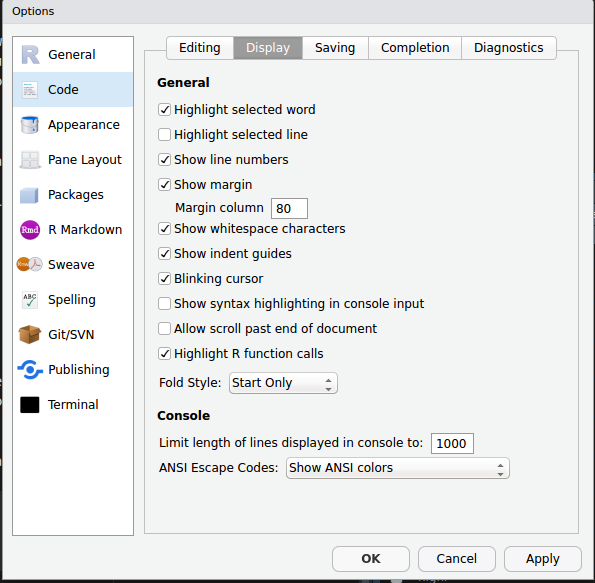
\includegraphics[width=0.5\linewidth]{options} 

}

\caption{Code display options}\label{fig:option-settings}
\end{figure}

\begin{itemize}
\tightlist
\item
  \emph{Highlight selected word}
\item
  \emph{Show line number}
\item
  \emph{Show margin} (and set margin column to 80)
\item
  \emph{Show whitespace characters}
\item
  \emph{Highlite R function calls}
\end{itemize}

Generally speaking those options, do not influence how your code is
performed, but will allow you to write cleaner and read easier. You can
also change colors of your environment in \emph{Appearance}.

\section{Installing packages}\label{installing-packages}

In your \emph{`Files'} window, you will find \emph{Packages} pane, which
contains \emph{Install} button. You can use it now, to install packages
needed to perform exercises from this book. The packages are:

\begin{figure}

{\centering 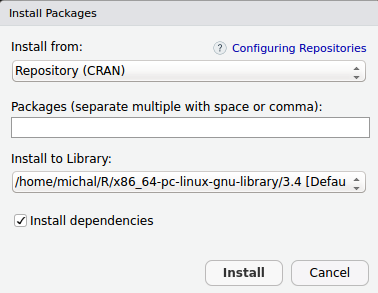
\includegraphics[width=0.5\linewidth]{instalPacks} 

}

\caption{Installation window}\label{fig:install-packs}
\end{figure}

\begin{itemize}
\tightlist
\item
  \textbf{deSolve} \citep{R-deSolve}
\item
  \textbf{fitdistrplus} \citep{R-fitdistrplus}
\item
  \textbf{mc2d} \citep{R-mc2d}
\item
  \textbf{minpack.lm} \citep{R-minpack.lm}
\item
  \textbf{nls2} \citep{R-nls2}
\item
  \textbf{nlsMicrobio} \citep{R-nlsMicrobio}
\item
  \textbf{segmented} \citep{R-segmented}
\item
  \textbf{tidyverse} \citep{R-tidyverse, R-dplyr, R-ggplot2, R-tidyr}
\end{itemize}

Now every time you need functions from specific package in library you
can just tick box next to package name, and RStudio will load it for
you.

\section{Conventions}\label{conventions}

In this book, we will use following conventions:

\begin{itemize}
\tightlist
\item
  Names of programs and packages are in \textbf{Bold}.
\item
  All other names e.g.~names of panes menu items as well as things that
  needs to be stressed are in \emph{italics}.
\item
  Function names and variables are always written in inline code e.g.
  \texttt{t.test()} or \texttt{x}.
\item
  File names are written in inline code e.g. \texttt{foo.txt}.
\item
  Citations are in APA style, and `clickable' e.g.click on the name and
  year of \textbf{knitr} package citation \citep{xie2015}.
\item
  Code chunks are in blocks and result lines start with \#\#
\end{itemize}

\begin{Shaded}
\begin{Highlighting}[]
\KeywordTok{rnorm}\NormalTok{(}\DecValTok{10}\NormalTok{, }\DecValTok{1}\NormalTok{, }\FloatTok{0.5}\NormalTok{)}
\end{Highlighting}
\end{Shaded}

\begin{verbatim}
##  [1] 1.2070236 0.2328131 1.1311709 1.4189133 1.2193364 1.0709074 1.2161778
##  [8] 1.3727643 0.8065509 0.6012342
\end{verbatim}

\begin{itemize}
\tightlist
\item
  There are no \texttt{\textgreater{}} (\emph{prompt}) signs in code
  chunks.
\item
  Figures are floating - meaning, that they are not always immediately
  after they are mentioned in text.
\item
  Tables are in \emph{longtable} format (meaning they are not floating
  and might be multipage) e.g.
\end{itemize}

\begin{Shaded}
\begin{Highlighting}[]
\NormalTok{knitr}\OperatorTok{::}\KeywordTok{kable}\NormalTok{(}
  \KeywordTok{head}\NormalTok{(iris, }\DecValTok{25}\NormalTok{), }\DataTypeTok{caption =} \StringTok{'Example table'}\NormalTok{,}
  \DataTypeTok{booktabs =} \OtherTok{TRUE}\NormalTok{, }\DataTypeTok{longtable =} \OtherTok{TRUE}
\NormalTok{)}
\end{Highlighting}
\end{Shaded}

\begin{longtable}[t]{rrrrl}
\caption{\label{tab:nice-tab}Example table}\\
\toprule
Sepal.Length & Sepal.Width & Petal.Length & Petal.Width & Species\\
\midrule
5.1 & 3.5 & 1.4 & 0.2 & setosa\\
4.9 & 3.0 & 1.4 & 0.2 & setosa\\
4.7 & 3.2 & 1.3 & 0.2 & setosa\\
4.6 & 3.1 & 1.5 & 0.2 & setosa\\
5.0 & 3.6 & 1.4 & 0.2 & setosa\\
\addlinespace
5.4 & 3.9 & 1.7 & 0.4 & setosa\\
4.6 & 3.4 & 1.4 & 0.3 & setosa\\
5.0 & 3.4 & 1.5 & 0.2 & setosa\\
4.4 & 2.9 & 1.4 & 0.2 & setosa\\
4.9 & 3.1 & 1.5 & 0.1 & setosa\\
\addlinespace
5.4 & 3.7 & 1.5 & 0.2 & setosa\\
4.8 & 3.4 & 1.6 & 0.2 & setosa\\
4.8 & 3.0 & 1.4 & 0.1 & setosa\\
4.3 & 3.0 & 1.1 & 0.1 & setosa\\
5.8 & 4.0 & 1.2 & 0.2 & setosa\\
\addlinespace
5.7 & 4.4 & 1.5 & 0.4 & setosa\\
5.4 & 3.9 & 1.3 & 0.4 & setosa\\
5.1 & 3.5 & 1.4 & 0.3 & setosa\\
5.7 & 3.8 & 1.7 & 0.3 & setosa\\
5.1 & 3.8 & 1.5 & 0.3 & setosa\\
\addlinespace
5.4 & 3.4 & 1.7 & 0.2 & setosa\\
5.1 & 3.7 & 1.5 & 0.4 & setosa\\
4.6 & 3.6 & 1.0 & 0.2 & setosa\\
5.1 & 3.3 & 1.7 & 0.5 & setosa\\
4.8 & 3.4 & 1.9 & 0.2 & setosa\\
\bottomrule
\end{longtable}

\begin{itemize}
\tightlist
\item
  Tables and figures and references are clickable e.g.~see Table
  \ref{tab:nice-tab} or see Figure \ref{fig:option-settings}.
\end{itemize}

\chapter{Basics}\label{basics}

In this chapter you will see some short introduction to \textbf{R}
environment. The basic information will be covered with more concern in
following chapters.

\section{Getting started}\label{getting-started}

\subsection{Help}\label{help}

There are just few things you really need to remember and follow when
you want to start using \textbf{R}. First, there is very good
\emph{help} build in. To access it, you use \texttt{?} sign with name of
function: e.g.: \texttt{?t.test}. After executing command, in your
window with \emph{Help} pane, a page dedicated to this function will pop
up. You will get information on syntax, options to use with this
function and in most cases some code examples. However, with single
question mark you are telling \textbf{R} to only look into functions
from packages that are \emph{currently loaded} and have this
\emph{precise name}. If you want to tell \textbf{R} to look for proper
function in \emph{all packages} or you are not sure what the exact name
is you can use double question mark e.g. \texttt{??mutate}. In effect,
in the same pane and window as previously you will get a list of results
that match your query. Finally, using \emph{Packages} pane, you can
click on one of the packages names, to display all of the functions
within it. Than, by clicking on the name of functions you are interested
in, you will be taken to proper page with description.

\subsection{Internet is a great source of
information}\label{internet-is-a-great-source-of-information}

Anytime you feel lost or need help that is beyond the scope of manuals,
just ask Google. For instance you can use this query: \emph{how to make
density plot in R}. Thanks to huge community you will find a lot of
answers. The most reliable ones can be found on \emph{StackOverflow},
\emph{StatsExchange} and \emph{RBloggers}. If you don't know if there is
a package to perform particular task, also ask uncle Google. For
instance, if you want to use random numbers from Dirichlet distribution,
you can use this query: \emph{dirichlet distribution r}.

\subsection{More on internet sources}\label{more-on-internet-sources}

A good practice, when you want to learn programming language, is to read
what other people do and how they code. In the beginning it might be a
bit overwhelming or confusing to read all the stuff. However, reading
others work will get you used to syntax and workflow, and will give you
great basics to invent your own code. Hopefully, you don't need to spend
hours searching for some interesting blogs. There is great blog
aggregator \href{https://rweekly.org}{R weekly}, that gathers in one
place the best posts, pod-casts, etc. on \textbf{R}, every week.

\section{Syntax}\label{syntax}

\subsection{Common operators}\label{common-operators}

In general \textbf{R} syntax resembles syntax of standard math functions
\(f(x, z) = a * x + b * z\). So in \textbf{R} the syntax to call this
function would be\ldots{} \texttt{f(x,\ z)}, which would evaluate
(behind scenes) expression \texttt{a\ *\ x\ +\ b\ *\ z}. You can think
about functions in this language with general pattern
\texttt{function\_name(argument\_1,\ argument\_2,\ ...,\ argument\_n)}.
Next thing you should know before you start working is that there are
three main \emph{signs} used in \textbf{R's} syntax. First two are
assignment symbols: \texttt{\textless{}-} and \texttt{=}; for convention
we use them in different cases. \textbf{You need to use \texttt{=} ONLY
for function arguments}. Third one is \texttt{\#}. It is a symbol used
for comments. Everything following this symbol to the end of code line
will not be executed. There are also other signs (or symbols) which are
building blocks of language, however their use is very precisely defined
and reserved for certain events. Below you find a table with reference
for most common operators used. You will faster grasp it while you write
your own code, than by reading about it. Thus, I suggest we go deeper
into variable types in \textbf{R} language.

\begin{longtable}[t]{lll}
\caption{\label{tab:tab-operators}Common operators in R}\\
\toprule
sign & type & action\\
\midrule
+ & maths & addition\\
- & maths & substraction\\
* & maths & multiplication\\
/ & maths & division\\
\%\% & maths & modulo\\
\addlinespace
\textasciicircum{} & maths & power\\
> & relations & left greater\\
>= & relations & left greater of equal\\
< & relations & right greater\\
<= & relations & right greater or equal\\
\addlinespace
== & relations & left equal right\\
!= & relations & left uneqal right\\
! & logics & not\\
\& & logics & and\\
| & logics & or\\
\addlinespace
\textasciitilde{} & model & left relates to right\\
<- or -> & assignment & assignes value to variable\\
\$ & address & extracts values with 'element name' from variable\\
: & sequence & creates sequence of numbers from 'left value' to 'right value'\\
\%>\% or \%<>\% & piping & pipes results(from left) as arguments to functionon right\\
\bottomrule
\end{longtable}

\subsection{Variables}\label{variables}

Concept of variable is crucial for programming. In \textbf{R} variables
can contain many things: vectors, data frames, results of statistical
analyses etc. Each of variables have some characteristic properties.
They are defined by \emph{class} of the variable. Thanks to \emph{class}
attribute, \textbf{R} knows, how to deal with variable -- what is the
internal structure and what operations can be performed over variable.
Data can be stored in variables in different manners. To assign
something to variable we use \texttt{\textless{}-} operator, which tells
\textbf{R} to store right side of arrow under name on the left side of
arrow. The simplest variable is \emph{vector}, which can be of
\emph{class}: \emph{character}, \emph{integer}, \emph{numeric} or
\emph{logical}. For instance:

\begin{Shaded}
\begin{Highlighting}[]
\NormalTok{characterVector <-}\StringTok{ }\KeywordTok{c}\NormalTok{(}\StringTok{'a'}\NormalTok{, }\StringTok{'b'}\NormalTok{, }\StringTok{'c'}\NormalTok{)}
\KeywordTok{class}\NormalTok{(characterVector)}
\end{Highlighting}
\end{Shaded}

\begin{verbatim}
## [1] "character"
\end{verbatim}

\begin{Shaded}
\begin{Highlighting}[]
\NormalTok{integerVector <-}\StringTok{ }\KeywordTok{c}\NormalTok{(1L, 2L, 3L)}
\KeywordTok{class}\NormalTok{(integerVector)}
\end{Highlighting}
\end{Shaded}

\begin{verbatim}
## [1] "integer"
\end{verbatim}

\begin{Shaded}
\begin{Highlighting}[]
\NormalTok{numericVector <-}\StringTok{ }\KeywordTok{c}\NormalTok{(}\FloatTok{2.5}\NormalTok{, }\FloatTok{3.5}\NormalTok{, }\FloatTok{4.5}\NormalTok{)}
\KeywordTok{class}\NormalTok{(numericVector)}
\end{Highlighting}
\end{Shaded}

\begin{verbatim}
## [1] "numeric"
\end{verbatim}

\begin{Shaded}
\begin{Highlighting}[]
\NormalTok{logicalVector <-}\StringTok{ }\KeywordTok{c}\NormalTok{(}\OtherTok{TRUE}\NormalTok{, }\OtherTok{FALSE}\NormalTok{)}
\KeywordTok{class}\NormalTok{(logicalVector)}
\end{Highlighting}
\end{Shaded}

\begin{verbatim}
## [1] "logical"
\end{verbatim}

For more complex data, we have four basic classes: \emph{vectors},
\emph{lists}, \emph{data frames} and \emph{matrices}. \emph{Matrix} is
similar to \emph{data frame}. The most obvious difference is that
\emph{matrix} contains only one \emph{class} of variables (usually
\emph{numeric} or \emph{integer}), while \emph{data frame} can store
\emph{numeric}, as well as \emph{characters} and \emph{factors} (for
now, you can assume that \emph{factor} class is used to store
categorical variables) in separate columns. Also \emph{matrices} are
used when programmers want to achieve great speed in mathematical
computation. \emph{Data frames} are resembling tables from popular
spreadsheet software. Lets look:

\begin{Shaded}
\begin{Highlighting}[]
\NormalTok{matrixVariable <-}\StringTok{ }\KeywordTok{matrix}\NormalTok{(}\KeywordTok{c}\NormalTok{(}\DecValTok{1}\OperatorTok{:}\DecValTok{10}\NormalTok{), }\DataTypeTok{nrow =} \DecValTok{2}\NormalTok{)}
\NormalTok{matrixVariable}
\end{Highlighting}
\end{Shaded}

\begin{verbatim}
##      [,1] [,2] [,3] [,4] [,5]
## [1,]    1    3    5    7    9
## [2,]    2    4    6    8   10
\end{verbatim}

\begin{Shaded}
\begin{Highlighting}[]
\KeywordTok{class}\NormalTok{(matrixVariable)}
\end{Highlighting}
\end{Shaded}

\begin{verbatim}
## [1] "matrix"
\end{verbatim}

\begin{Shaded}
\begin{Highlighting}[]
\NormalTok{dfVariable <-}\StringTok{ }\KeywordTok{data.frame}\NormalTok{(}\DataTypeTok{x1 =} \DecValTok{1}\OperatorTok{:}\DecValTok{5}\NormalTok{, }\DataTypeTok{x2 =} \DecValTok{6}\OperatorTok{:}\DecValTok{10}\NormalTok{)}
\NormalTok{dfVariable}
\end{Highlighting}
\end{Shaded}

\begin{verbatim}
##   x1 x2
## 1  1  6
## 2  2  7
## 3  3  8
## 4  4  9
## 5  5 10
\end{verbatim}

\begin{Shaded}
\begin{Highlighting}[]
\KeywordTok{class}\NormalTok{(dfVariable)}
\end{Highlighting}
\end{Shaded}

\begin{verbatim}
## [1] "data.frame"
\end{verbatim}

\emph{Lists} are\ldots{} lists of variables. Each \emph{list} element
can be of different \emph{class} and length. To grasp the idea of
\emph{lists} it will be best to present it with example:

\begin{Shaded}
\begin{Highlighting}[]
\NormalTok{listVariable <-}\StringTok{ }\KeywordTok{list}\NormalTok{(}\DataTypeTok{x1 =} \KeywordTok{c}\NormalTok{(}\StringTok{"a"}\NormalTok{, }\StringTok{"b"}\NormalTok{), }\DataTypeTok{x2 =} \DecValTok{1}\OperatorTok{:}\DecValTok{4}\NormalTok{, }\DataTypeTok{x3 =} \KeywordTok{matrix}\NormalTok{(}\KeywordTok{c}\NormalTok{(}\DecValTok{1}\OperatorTok{:}\DecValTok{6}\NormalTok{), }\DataTypeTok{nrow =} \DecValTok{2}\NormalTok{))}
\NormalTok{listVariable}
\end{Highlighting}
\end{Shaded}

\begin{verbatim}
## $x1
## [1] "a" "b"
## 
## $x2
## [1] 1 2 3 4
## 
## $x3
##      [,1] [,2] [,3]
## [1,]    1    3    5
## [2,]    2    4    6
\end{verbatim}

\begin{Shaded}
\begin{Highlighting}[]
\KeywordTok{class}\NormalTok{(listVariable)}
\end{Highlighting}
\end{Shaded}

\begin{verbatim}
## [1] "list"
\end{verbatim}

\begin{Shaded}
\begin{Highlighting}[]
\KeywordTok{class}\NormalTok{(listVariable}\OperatorTok{$}\NormalTok{x1)}
\end{Highlighting}
\end{Shaded}

\begin{verbatim}
## [1] "character"
\end{verbatim}

\begin{Shaded}
\begin{Highlighting}[]
\KeywordTok{class}\NormalTok{(listVariable}\OperatorTok{$}\NormalTok{x2)}
\end{Highlighting}
\end{Shaded}

\begin{verbatim}
## [1] "integer"
\end{verbatim}

\begin{Shaded}
\begin{Highlighting}[]
\KeywordTok{class}\NormalTok{(listVariable}\OperatorTok{$}\NormalTok{x3)}
\end{Highlighting}
\end{Shaded}

\begin{verbatim}
## [1] "matrix"
\end{verbatim}

There are plenty of other \emph{classes}, e.g.~for \emph{time
variables}, however mentioned above are the basic ones you will deal
mostly. Also because they are so often used, you should learn how to
recognize their structure at a glance. Later on, I will present you how
(and when) each of this variables types can be used in work.

\subsubsection{Naming Variables}\label{naming-variables}

First of all, all names are \emph{case-sensitive}, which means that
\textbf{R} recognize variables named \texttt{RVariable},
\texttt{rVariable} and \texttt{Rvariable} as three different objects.
Second thing to remember is that variable name \emph{have to} start with
a letter and may contain only letters, numbers and symbols: . (dot) and
\_ (underscore). There are also some \emph{good practices} in naming
variables (after \href{http://adv-r.had.com.nz/Style.html}{Hadley
Wickham Style guide}):

\begin{itemize}
\tightlist
\item
  use lowercase to names variables (and functions)
\item
  use nouns to name variables (and verbs for functions)
\item
  try to be precise when naming
\item
  try to be concise when naming
\item
  use underscore \_ to separate words (snake\_case) e.g.
  \texttt{first\_variable}
\item
  \emph{some other guidelines suggest using camel cases e.g.}
  \texttt{firstVariable}
\end{itemize}

And the golden rule should be - whatever guideline you follow -- be
consequent!

\section{Math operations}\label{math-operations}

In \textbf{R} we use standard math operators \texttt{+\ -\ *\ /} to
perform addition, subtraction, multiplication and division. Symbol
\texttt{\^{}} indicates that we want to use power, and \texttt{sqrt} to
make square root. OK, so whats the name of a function to get
n\textsuperscript{th} root? Probably you remember from math lessons that
\(\sqrt [n] {x} = x^\frac{1}{n}\), thus you can just write
\texttt{x\^{}(1/n)}. To change order of operation (which are following
mathematics rules) use brackets \texttt{()}. Other important
mathematical functions are \texttt{\%\%} for modulo, and \texttt{\%/\%}
for integer division.

\begin{Shaded}
\begin{Highlighting}[]
\DecValTok{5} \OperatorTok{+}\StringTok{ }\DecValTok{2}
\end{Highlighting}
\end{Shaded}

\begin{verbatim}
## [1] 7
\end{verbatim}

\begin{Shaded}
\begin{Highlighting}[]
\DecValTok{11} \OperatorTok{-}\StringTok{ }\DecValTok{3}
\end{Highlighting}
\end{Shaded}

\begin{verbatim}
## [1] 8
\end{verbatim}

\begin{Shaded}
\begin{Highlighting}[]
\NormalTok{(}\DecValTok{4}\OperatorTok{+}\DecValTok{7}\NormalTok{)}\OperatorTok{/}\DecValTok{9}\OperatorTok{*}\DecValTok{2}
\end{Highlighting}
\end{Shaded}

\begin{verbatim}
## [1] 2.444444
\end{verbatim}

\begin{Shaded}
\begin{Highlighting}[]
\DecValTok{14} \OperatorTok\StringTok{ }\DecValTok{3} \OperatorTok{+}\StringTok{ }\DecValTok{1}
\end{Highlighting}
\end{Shaded}

\begin{verbatim}
## [1] 5
\end{verbatim}

\begin{Shaded}
\begin{Highlighting}[]
\DecValTok{8}\OperatorTok{^}\NormalTok{(}\DecValTok{1}\OperatorTok{/}\DecValTok{3}\NormalTok{) }\OperatorTok{+}\StringTok{ }\DecValTok{10}\OperatorTok\DecValTok{6}
\end{Highlighting}
\end{Shaded}

\begin{verbatim}
## [1] 6
\end{verbatim}

To calculate logarithms there is \emph{build in} function
\texttt{log()}. It uses as a base Euler's number by default, however you
can override it i.e. \texttt{log(10,\ base\ =\ 10)}. You can calculate
exponential function using \texttt{exp()} function. There are also
trigonometric functions in \textbf{R}: \texttt{sin()}, \texttt{cos()},
\texttt{tan()}, \texttt{asin()}, \texttt{acos()}, \texttt{atan()}.
Angles are used/expressed in radians. To transform values from degrees
to radians multiply by \texttt{pi} and divide by 180. To transform
values from radians to degrees multiply by 180 and divide by
\texttt{pi}. By the way, \texttt{pi} is a constant in \textbf{R},
meaning that its value is build in the language (similar as Euler number
is \texttt{exp(1)}).

\begin{Shaded}
\begin{Highlighting}[]
\NormalTok{someArc <-}\StringTok{ }\DecValTok{90}\OperatorTok{*}\NormalTok{pi}\OperatorTok{/}\DecValTok{180}
\KeywordTok{sin}\NormalTok{(someArc)}
\end{Highlighting}
\end{Shaded}

\begin{verbatim}
## [1] 1
\end{verbatim}

\begin{Shaded}
\begin{Highlighting}[]
\NormalTok{atanValue <-}\StringTok{ }\KeywordTok{atan}\NormalTok{(}\FloatTok{0.89}\NormalTok{)}
\NormalTok{atanValue}\OperatorTok{*}\DecValTok{180}\OperatorTok{/}\NormalTok{pi}
\end{Highlighting}
\end{Shaded}

\begin{verbatim}
## [1] 41.66908
\end{verbatim}

\section{Logics}\label{logics}

Logical expression are often used in programming. They compare left side
with right side arguments of statement. The result of those comparison
might be \texttt{TRUE} or \texttt{FALSE} (in many other languages those
are called \emph{Boolean} values) which belong to \emph{class Logical}.
In Table \ref{tab:tab-operators} you will find list of most common
logical operators used to build statements. Here is a small
\emph{cheatsheet tables}:

\begin{longtable}[t]{llll}
\caption{\label{tab:tab-logics}AND Table}\\
\toprule
  & NA & FALSE & TRUE\\
\midrule
NA & NA & FALSE & NA\\
FALSE & FALSE & FALSE & FALSE\\
TRUE & NA & FALSE & TRUE\\
\bottomrule
\end{longtable}

\begin{longtable}[t]{llll}
\caption{\label{tab:tab-logics}OR Table}\\
\toprule
  & NA & FALSE & TRUE\\
\midrule
NA & NA & NA & TRUE\\
FALSE & NA & FALSE & TRUE\\
TRUE & TRUE & TRUE & TRUE\\
\bottomrule
\end{longtable}

Below you can see them in action:

\begin{Shaded}
\begin{Highlighting}[]
\DecValTok{5} \OperatorTok{>=}\StringTok{ }\DecValTok{1}
\end{Highlighting}
\end{Shaded}

\begin{verbatim}
## [1] TRUE
\end{verbatim}

\begin{Shaded}
\begin{Highlighting}[]
\DecValTok{10}\OperatorTok\DecValTok{2} \OperatorTok{==}\StringTok{ }\DecValTok{0}
\end{Highlighting}
\end{Shaded}

\begin{verbatim}
## [1] TRUE
\end{verbatim}

\begin{Shaded}
\begin{Highlighting}[]
\OperatorTok{!}\OtherTok{FALSE}
\end{Highlighting}
\end{Shaded}

\begin{verbatim}
## [1] TRUE
\end{verbatim}

\begin{Shaded}
\begin{Highlighting}[]
\NormalTok{5L }\OperatorTok{|}\StringTok{ }\FloatTok{11.1} \OperatorTok{<=}\StringTok{ }\DecValTok{6}
\end{Highlighting}
\end{Shaded}

\begin{verbatim}
## [1] TRUE
\end{verbatim}

\section{Functions}\label{functions}

When writing code we generally want to perform some actions on our
variables. There is a lot of \emph{build in functions} in base
\textbf{R} distribution, and a whole Galaxy of \emph{functions} provided
by community. Function can be literally any action performed on
variables. For instance, there are some build in statistical functions
like \texttt{t.test()} or \texttt{chisq.test()}. Other function can be
use to draw some charts and plots, e.g. \texttt{plot()}. It's easy to
recognize function, since its structure is \emph{name} followed by
parentheses \emph{()}. Inside parentheses user provides arguments and
options to function. Lets see how it works with one of \emph{build in}
functions:

\begin{Shaded}
\begin{Highlighting}[]
\NormalTok{tTestResult <-}\StringTok{ }\KeywordTok{t.test}\NormalTok{(numericVector, integerVector)}
\KeywordTok{print}\NormalTok{(tTestResult)}
\end{Highlighting}
\end{Shaded}

\begin{verbatim}
## 
##  Welch Two Sample t-test
## 
## data:  numericVector and integerVector
## t = 1.8371, df = 4, p-value = 0.1401
## alternative hypothesis: true difference in means is not equal to 0
## 95 percent confidence interval:
##  -0.7669579  3.7669579
## sample estimates:
## mean of x mean of y 
##       3.5       2.0
\end{verbatim}

We used \texttt{t.test()} function, with two arguments:
\texttt{numericVector} and \texttt{integerVector}. In second function
call, we \emph{ordered} \textbf{R} to print out the results of
statistical test stored in variable \texttt{tTestResult} -- which is the
argument of this function. I'll show you how to write your own function
in chapter \ref{functions}.

\chapter{Somwehere between basic and
useful}\label{somwehere-between-basic-and-useful}

\section{Addressing}\label{addressing}

\subsection{Vectors}\label{vectors}

When you deal with variables you often will want to use only a part of
it in your work. Other times you will want to get rid of some values
which follow certain criteria. In order to do it you need to know an
`address' of particular value in a \emph{vector}, \emph{data frame},
\emph{list} etc. From now on, I will use some functions while describing
it \emph{at hoc}, since I believe the best way to learn them, is to use
them. Lets create a \emph{vector} and see what we can do with it.

\begin{Shaded}
\begin{Highlighting}[]
\NormalTok{addressVec <-}\StringTok{ }\KeywordTok{seq}\NormalTok{(}\DataTypeTok{from =} \DecValTok{1}\NormalTok{, }\DataTypeTok{to =} \DecValTok{20}\NormalTok{, }\DataTypeTok{by =} \DecValTok{2}\NormalTok{)}
\NormalTok{addressVec}
\end{Highlighting}
\end{Shaded}

\begin{verbatim}
##  [1]  1  3  5  7  9 11 13 15 17 19
\end{verbatim}

Instead of typing all the numbers by hand, we can use \texttt{seq()}
function, to generate it automatically. This function takes two
arguments \texttt{from} and \texttt{to}, however additionally we can use
option \texttt{by} which defines increment of the sequence. As your
knowledge is growing I can tell you a secret. Often, there is no need to
name all the arguments and options in functions body. In the beginning
you should use the names, but the more experienced you get, you will
notice that you omit them often. Actually we nearly always omit so
called \emph{default} options of a function. Use \texttt{?seq} to check
the help page for this function. You will see that it can take more
options than \texttt{from}, \texttt{to} and \texttt{by}, but since they
are predefined we don't need to bother and type them (as long as we are
OK with \emph{default} settings). So, lets retype our \emph{variable}
definition:

\begin{Shaded}
\begin{Highlighting}[]
\NormalTok{addressVec <-}\StringTok{ }\KeywordTok{seq}\NormalTok{(}\DecValTok{1}\NormalTok{, }\DecValTok{20}\NormalTok{, }\DecValTok{2}\NormalTok{)}
\NormalTok{addressVec}
\end{Highlighting}
\end{Shaded}

\begin{verbatim}
##  [1]  1  3  5  7  9 11 13 15 17 19
\end{verbatim}

The results are identical. Lets get back to addressing issues. Suppose
you want to check the fifth element of our \texttt{addressVec} variable.
To do it we use variable name followed by element number in brackets (or
square brackets, if you will).

\begin{Shaded}
\begin{Highlighting}[]
\NormalTok{addressVec[}\DecValTok{5}\NormalTok{]}
\end{Highlighting}
\end{Shaded}

\begin{verbatim}
## [1] 9
\end{verbatim}

If you want to get rid of fifth element just precede it with \texttt{-}.

\begin{Shaded}
\begin{Highlighting}[]
\NormalTok{addressVec[}\OperatorTok{-}\DecValTok{5}\NormalTok{]}
\end{Highlighting}
\end{Shaded}

\begin{verbatim}
## [1]  1  3  5  7 11 13 15 17 19
\end{verbatim}

Easy. The thing that is worth to mention right now is that \textbf{R
Core Team} have reason and dignity of human beings so they start
numeration of elements with value 1. In some other languages, because of
no sensible reasons, numeration starts with 0 -- which is horribly
annoying. What to do if we want to extract values of more than one
element?

\begin{Shaded}
\begin{Highlighting}[]
\NormalTok{addressVec[}\DecValTok{1}\NormalTok{,}\DecValTok{5}\NormalTok{]}
\end{Highlighting}
\end{Shaded}

\begin{verbatim}
## Error in addressVec[1, 5]: incorrect number of dimensions
\end{verbatim}

\begin{Shaded}
\begin{Highlighting}[]
\NormalTok{addressVec[}\OperatorTok{-}\DecValTok{1}\NormalTok{,}\OperatorTok{-}\DecValTok{5}\NormalTok{,}\OperatorTok{-}\DecValTok{6}\NormalTok{]}
\end{Highlighting}
\end{Shaded}

\begin{verbatim}
## Error in addressVec[-1, -5, -6]: incorrect number of dimensions
\end{verbatim}

Error occurs with warning that there is incorrect number of dimensions.
That's because \emph{vectors} have only one dimension -- length. Within
square brackets comma separates dimensions. So when we used command
\texttt{{[}1,5{]}} we told R to look for value that address is number 1
in first dimension and number 5 in second dimension. To correct the
mistake, we need to provide a vector of numbers from first dimension. We
can use \texttt{c()} function to create \emph{ad hoc vector} inside
square brackets.

\begin{Shaded}
\begin{Highlighting}[]
\NormalTok{addressVec[}\KeywordTok{c}\NormalTok{(}\DecValTok{1}\NormalTok{,}\DecValTok{5}\NormalTok{)]}
\end{Highlighting}
\end{Shaded}

\begin{verbatim}
## [1] 1 9
\end{verbatim}

\begin{Shaded}
\begin{Highlighting}[]
\NormalTok{addressVec[}\OperatorTok{-}\KeywordTok{c}\NormalTok{(}\DecValTok{1}\NormalTok{,}\DecValTok{5}\NormalTok{,}\DecValTok{6}\NormalTok{)]}
\end{Highlighting}
\end{Shaded}

\begin{verbatim}
## [1]  3  5  7 13 15 17 19
\end{verbatim}

Now something more complicated. Try to figure out what code below does,
and what is the result of \texttt{which()} function:

\begin{Shaded}
\begin{Highlighting}[]
\NormalTok{addressVec[}\KeywordTok{which}\NormalTok{(addressVec }\OperatorTok{>=}\StringTok{ }\DecValTok{6}\NormalTok{)] <-}\StringTok{ 'o..O'}
\NormalTok{addressVec}
\end{Highlighting}
\end{Shaded}

\begin{verbatim}
##  [1] "1"    "3"    "5"    "o..O" "o..O" "o..O" "o..O" "o..O" "o..O" "o..O"
\end{verbatim}

If you have problems, you can think of this example as a composition of
actions. First there is expression
\texttt{addressVec\ \textgreater{}=6}, than we use \texttt{which()}
function with argument from previous expression. Next the result is
passed as an address. Last thing is assignment of new value to\ldots{}

\subsection{Data frames (and matrices)}\label{data-frames-and-matrices}

When dealing with \emph{data frames}, addressing is possible in two
ways. First is similar to \emph{vector} addressing. However, as
\emph{data frames} have two dimensions, you will need to express them
like \texttt{df{[}1,\ 2{]}} -- which tells \textbf{R} to look up the
cell in row 1, column 2. But what if you want to check all the cells in
particular row or column? Omit the number, but not the coma -- like
this: \texttt{df{[},\ 3{]}}. It will display all row values from column
3. And of course you can still use \emph{vectors} when addressing. This
way also works for \emph{matrices}.

\begin{Shaded}
\begin{Highlighting}[]
\NormalTok{addressDF <-}\StringTok{ }\KeywordTok{data.frame}\NormalTok{(}\DataTypeTok{C1 =} \KeywordTok{seq}\NormalTok{(}\DecValTok{1}\NormalTok{,}\DecValTok{10}\NormalTok{), }\DataTypeTok{C2 =} \KeywordTok{seq}\NormalTok{(}\DecValTok{11}\NormalTok{,}\DecValTok{20}\NormalTok{), }\DataTypeTok{C3 =} \KeywordTok{seq}\NormalTok{(}\DecValTok{21}\NormalTok{,}\DecValTok{30}\NormalTok{))}
\NormalTok{addressDF[}\DecValTok{5}\NormalTok{, }\DecValTok{2}\NormalTok{]}
\end{Highlighting}
\end{Shaded}

\begin{verbatim}
## [1] 15
\end{verbatim}

\begin{Shaded}
\begin{Highlighting}[]
\NormalTok{addressDF[}\DecValTok{6}\NormalTok{, ]}
\end{Highlighting}
\end{Shaded}

\begin{verbatim}
##   C1 C2 C3
## 6  6 16 26
\end{verbatim}

\begin{Shaded}
\begin{Highlighting}[]
\NormalTok{addressDF[}\KeywordTok{c}\NormalTok{(}\DecValTok{6}\NormalTok{, }\DecValTok{7}\NormalTok{), }\DecValTok{1}\OperatorTok{:}\DecValTok{3}\NormalTok{]}
\end{Highlighting}
\end{Shaded}

\begin{verbatim}
##   C1 C2 C3
## 6  6 16 26
## 7  7 17 27
\end{verbatim}

The second option is to use \texttt{\$} sign followed with column name
(and it works only for \emph{data frames} and \emph{lists}). This way,
we tell \textbf{R} to look in whole column. If we want to display values
from particular cells, we put them in brackets after column name, the
same way as we do for \emph{vectors}:

\begin{Shaded}
\begin{Highlighting}[]
\NormalTok{addressDF}\OperatorTok{$}\NormalTok{C2[}\DecValTok{5}\NormalTok{]}
\end{Highlighting}
\end{Shaded}

\begin{verbatim}
## [1] 15
\end{verbatim}

\begin{Shaded}
\begin{Highlighting}[]
\NormalTok{addressDF}\OperatorTok{$}\NormalTok{C3[}\KeywordTok{c}\NormalTok{(}\DecValTok{6}\OperatorTok{:}\DecValTok{9}\NormalTok{)]}
\end{Highlighting}
\end{Shaded}

\begin{verbatim}
## [1] 26 27 28 29
\end{verbatim}

When working with \emph{matrices} you will find a lot of functions that
apply to them (check help page for \texttt{base} package). The one you
should familiarize with, if you plan on working with \emph{matrix}
operations are:

\begin{itemize}
\tightlist
\item
  \texttt{dim()} -- returns dimensions of \emph{matrix}
\item
  \texttt{rownames()} and \texttt{colnames()} -- to specify row and
  column names
\item
  \texttt{cbind()} and \texttt{rbind()} -- to add columns or rows to a
  \emph{matrix} (respectively)
\item
  \texttt{lower.tri()}, \texttt{upper.tri()} -- lower and upper
  triangular part of \emph{matrix}
\item
  \texttt{t()} -- \emph{matrix} transposition
\item
  \texttt{outer()} -- outer products of \emph{matrix}
\item
  \texttt{rowsums()}, \texttt{rowmeans()}. \texttt{colsums()} and
  \texttt{colmeans()} -- tool to calculate sum and mean of rows or
  columns
\item
  \texttt{\%*\%} -- \emph{matrix} multiplication operator
  (\texttt{matrixOne\ \%*\%\ matrix2})
\item
  \texttt{diag()} -- diagonals of a \emph{matrix}
\end{itemize}

You can also check \emph{help} for \texttt{Matrix} package which
contains dozens of functions to deal with \emph{matrix} algebra and
\emph{matrix} transformations.

\subsection{Lists}\label{lists}

As mentioned before each \emph{list} element can have different
structure. Thus, addressing is kind of a mixture of all above. First you
need to address element of your \emph{list}. You do it with double
brackets containing element number following name of variable. You can
also use \texttt{\$} sign with name of the element. Than you use
addressing the same way you address \emph{data frames}, \emph{vectors}
or \emph{matrices}.

\begin{Shaded}
\begin{Highlighting}[]
\NormalTok{addressList <-}\StringTok{ }\KeywordTok{list}\NormalTok{(}\DataTypeTok{x1 =} \KeywordTok{c}\NormalTok{(}\StringTok{'a'}\NormalTok{, }\StringTok{'b'}\NormalTok{), }\DataTypeTok{x2 =} \DecValTok{1}\OperatorTok{:}\DecValTok{4}\NormalTok{, }\DataTypeTok{x3 =} \KeywordTok{matrix}\NormalTok{(}\KeywordTok{c}\NormalTok{(}\DecValTok{1}\OperatorTok{:}\DecValTok{6}\NormalTok{), }\DataTypeTok{nrow =} \DecValTok{2}\NormalTok{))}
\NormalTok{addressList[[}\DecValTok{2}\NormalTok{]]}
\end{Highlighting}
\end{Shaded}

\begin{verbatim}
## [1] 1 2 3 4
\end{verbatim}

\begin{Shaded}
\begin{Highlighting}[]
\NormalTok{addressList}\OperatorTok{$}\NormalTok{x2[}\DecValTok{3}\NormalTok{]}
\end{Highlighting}
\end{Shaded}

\begin{verbatim}
## [1] 3
\end{verbatim}

\begin{Shaded}
\begin{Highlighting}[]
\NormalTok{addressList[[}\DecValTok{3}\NormalTok{]]}
\end{Highlighting}
\end{Shaded}

\begin{verbatim}
##      [,1] [,2] [,3]
## [1,]    1    3    5
## [2,]    2    4    6
\end{verbatim}

\begin{Shaded}
\begin{Highlighting}[]
\NormalTok{addressList[[}\DecValTok{3}\NormalTok{]][, }\DecValTok{3}\NormalTok{]}
\end{Highlighting}
\end{Shaded}

\begin{verbatim}
## [1] 5 6
\end{verbatim}

OK, now simple task for you. There is a function called
\texttt{colnames()} which allow us to change names in \emph{matrix}
variable. To use it you need to put name of \emph{matrix} variable in
the parentheses (like this: \texttt{colnames(x)}), and assign value to
it (e.g.
\texttt{colnames(x)\ \textless{}-\ c(\textquotesingle{}one\textquotesingle{},\ \textquotesingle{}two\textquotesingle{})).\ Now\ change\ names\ of\ of\ columns\ in\ *matrix*\ that\ is\ element\ of\ list\ above\ to}I`,
`Love', `R'.

\section{Control flow}\label{control-flow}

Controlling flow of function, script or whole program is the essence of
programming. In general we can divide procedures in two big categories:
\textbf{conditional control} and \textbf{iteration control}. In the
first category we will find \texttt{if...else} statements. They change
execution of code depending on state of input or previous results. In
the second category we will find tools to repeatedly do execute some
code. Typically tools to control repeating of code are \texttt{for} and
\texttt{while} loops. However, in R there are special functions, which
are basically \texttt{for} loops but have slightly better performance,
and are shorter to write. We call them \texttt{apply} functions family.

\subsection{\texorpdfstring{\texttt{if...else} and \texttt{ifelse}
statments}{if...else and ifelse statments}}\label{if...else-and-ifelse-statments}

The simplest way to control how the code is executed are conditions. In
an abstract form it is something like telling your machine: if the state
is red make it blue, else make it green. The most general form it is
written like below:

\begin{Shaded}
\begin{Highlighting}[]
\ControlFlowTok{if}\NormalTok{ (x) \{ }\CommentTok{#writting just X without any condtition is evaluated as x == TRUE}
  \ControlFlowTok{function}\NormalTok{(x)}
\NormalTok{\}}
\NormalTok{####rest of the code####}

\CommentTok{#Or...}
\ControlFlowTok{if}\NormalTok{ (x) \{}
  \ControlFlowTok{function}\NormalTok{(x)}
\NormalTok{\} }\ControlFlowTok{else}\NormalTok{ \{ }\CommentTok{#in this example this block will be evaluated if x == FALSE}
  \ControlFlowTok{function}\NormalTok{(y)}
\NormalTok{\}}
\end{Highlighting}
\end{Shaded}

As you see, writing conditionals in their basic form is quite easy. If
our script can be in just on of two different states while it start
evaluating conditions both of above examples will be suitable. In
practice it happens quite often that we need to plan different actions
because of dichotomy in the results of previous actions. If our code in
this place is going to make some simple things you can consider using
\texttt{ifelse()} shortcut. It works like below:

\begin{Shaded}
\begin{Highlighting}[]
\NormalTok{coinToss <-}\StringTok{ }\KeywordTok{sample}\NormalTok{(}\KeywordTok{c}\NormalTok{(}\DecValTok{0}\NormalTok{,}\DecValTok{1}\NormalTok{), }\DecValTok{3}\NormalTok{, }\DataTypeTok{replace =}\NormalTok{ T)}
\NormalTok{coinToss}
\end{Highlighting}
\end{Shaded}

\begin{verbatim}
## [1] 1 1 1
\end{verbatim}

\begin{Shaded}
\begin{Highlighting}[]
\KeywordTok{ifelse}\NormalTok{(coinToss }\OperatorTok{>}\StringTok{ }\DecValTok{0}\NormalTok{, }\StringTok{'Win!'}\NormalTok{, }\StringTok{'Looser!'}\NormalTok{)}
\end{Highlighting}
\end{Shaded}

\begin{verbatim}
## [1] "Win!" "Win!" "Win!"
\end{verbatim}

But what if your script can have more than two states when you start
evaluating conditions? You will need to use \texttt{else\ if()}
structure. A simple example is below:

\begin{Shaded}
\begin{Highlighting}[]
\NormalTok{coinToss <-}\StringTok{ }\KeywordTok{sample}\NormalTok{(}\KeywordTok{c}\NormalTok{(}\DecValTok{0}\NormalTok{,}\DecValTok{1}\NormalTok{), }\DecValTok{3}\NormalTok{, }\DataTypeTok{replace =}\NormalTok{ T)}
\NormalTok{sumOfCoins <-}\StringTok{ }\KeywordTok{sum}\NormalTok{(coinToss)}\CommentTok{# we can have four states here 0,1,2,3}
\NormalTok{sumOfCoins}
\end{Highlighting}
\end{Shaded}

\begin{verbatim}
## [1] 1
\end{verbatim}

\begin{Shaded}
\begin{Highlighting}[]
\ControlFlowTok{if}\NormalTok{ (sumOfCoins }\OperatorTok{==}\StringTok{ }\DecValTok{0}\NormalTok{) \{}
  \StringTok{'Looser'}
\NormalTok{\} }\ControlFlowTok{else} \ControlFlowTok{if}\NormalTok{ (sumOfCoins }\OperatorTok{==}\StringTok{ }\DecValTok{1}\NormalTok{) \{}
  \StringTok{'Barely alive'}
\NormalTok{\} }\ControlFlowTok{else} \ControlFlowTok{if}\NormalTok{ (sumOfCoins }\OperatorTok{>=}\StringTok{ }\DecValTok{2}\NormalTok{) \{}
  \StringTok{'Big Winner!!!'}
\NormalTok{\}}
\end{Highlighting}
\end{Shaded}

\begin{verbatim}
## [1] "Barely alive"
\end{verbatim}

\begin{Shaded}
\begin{Highlighting}[]
\CommentTok{#Or because the functions realting to particular conditions are simple, you}
\CommentTok{#can make nested ifelse}
\KeywordTok{ifelse}\NormalTok{(}\KeywordTok{sum}\NormalTok{(sumOfCoins) }\OperatorTok{==}\StringTok{ }\DecValTok{0}\NormalTok{, }\StringTok{'Looser'}\NormalTok{,}
       \KeywordTok{ifelse}\NormalTok{(}\KeywordTok{sum}\NormalTok{(sumOfCoins) }\OperatorTok{==}\StringTok{ }\DecValTok{1}\NormalTok{, }\StringTok{'Barely alive'}\NormalTok{, }\StringTok{'Big Winner!!!'}\NormalTok{))}
\end{Highlighting}
\end{Shaded}

\begin{verbatim}
## [1] "Barely alive"
\end{verbatim}

\subsection{\texorpdfstring{\texttt{for} and \texttt{while}
loops}{for and while loops}}\label{for-and-while-loops}

In many cases we want to use the same function over data stored in
different \emph{vectors}, columns or data sets. Other time we need to
make sequence of computations in which every result depends on the
previous one (like, for instance, in
\href{https://en.wikipedia.org/wiki/Fibonacci_number}{Fibonacci
sequence}). In yet another situation we need to run function over data
set, but only till we reach specific value. Of course, we can do
everything manually, by copy-pasting code, taping \emph{ctrl+enter}
several times and so on. In every programming language we will find
tools that help us automatize this procedures, and by side effect make
them less prone to error. Those are called loops. Namely, the most
common loops used are \texttt{for} and \texttt{while}. The difference
between them, is that in first one we define number of iterations and in
the second one we define condition that must be met so the loops is
executed. In other words \texttt{for\ (i\ in\ 1:10)\ \{x\ +\ i\}} means
that numbers from 1 to 10 will be added to x in a sequence.
\texttt{while\ (x\ \textless{}\ 5)\ \{print(x\ \textless{}-\ x\ -\ 1)\}}
on the other hand will subtract value \texttt{1} from \texttt{x} as long
as \texttt{x} is greater than \texttt{0}. You thing that is worth to
mention is that \texttt{while} loops are general form and \texttt{for}
loops are special cases. It means that it is possible to rewrite any
\texttt{for} loop into \texttt{while} loop, but not the other way.

Also when working in loops you should always preallocate memory for your
output. In simple words it means, that if you are writing loop, that
grows the vector instead of just substitute values, \textbf{R} needs to
copy your previous results in each iteration. Thus making a
\emph{vector} of length of your number of iterations (or a \emph{list})
before you start a loop will save you some computational time.

To illustrate how it works in practice lets look on some simple
examples:

\begin{Shaded}
\begin{Highlighting}[]
\NormalTok{exampleDF <-}\StringTok{ }\KeywordTok{data.frame}\NormalTok{(}\DataTypeTok{norm =} \KeywordTok{rnorm}\NormalTok{(}\DecValTok{100}\NormalTok{, }\DecValTok{5}\NormalTok{, }\FloatTok{1.5}\NormalTok{),}
                        \DataTypeTok{chisq =} \KeywordTok{rchisq}\NormalTok{(}\DecValTok{100}\NormalTok{, }\DecValTok{3}\NormalTok{),}
                        \DataTypeTok{pois =} \KeywordTok{rpois}\NormalTok{(}\DecValTok{100}\NormalTok{, }\FloatTok{3.33}\NormalTok{))}
\NormalTok{distroMeans <-}\StringTok{ }\KeywordTok{vector}\NormalTok{(}\StringTok{'list'}\NormalTok{, }\KeywordTok{length}\NormalTok{(exampleDF)) }\CommentTok{#prealocate space}

\ControlFlowTok{for}\NormalTok{ (i }\ControlFlowTok{in} \KeywordTok{seq_along}\NormalTok{(exampleDF)) \{}
\NormalTok{  distroMeans[[i]] <-}\StringTok{ }\KeywordTok{summary}\NormalTok{(exampleDF[[i]])}
\NormalTok{\}}

\NormalTok{distroMeans}
\end{Highlighting}
\end{Shaded}

\begin{verbatim}
## [[1]]
##    Min. 1st Qu.  Median    Mean 3rd Qu.    Max. 
##   1.369   4.168   5.163   5.016   5.934   9.251 
## 
## [[2]]
##     Min.  1st Qu.   Median     Mean  3rd Qu.     Max. 
##  0.06683  1.41942  2.55623  3.38705  4.91848 15.39488 
## 
## [[3]]
##    Min. 1st Qu.  Median    Mean 3rd Qu.    Max. 
##    0.00    2.00    3.00    3.22    4.00    8.00
\end{verbatim}

Above example is very simple, and actually can be made without loop. Try
to call from your console following command \texttt{summary(exampleDF)}.
This is called vectorization which will be explained few paragraphs
below.

But lets get back to loops and write something that might be useful (yet
very simple). Assume that you are investigating animals reproduction.
You have a herd that counts 60 animals. The reproduction factor is
\texttt{1.34}, and survival factor is `0.75'. So the overall growth
factor can be calculated as \emph{reproduction factor} * \emph{survival
factor}. In each generation there is some noise in reproduction,
i.e.~from -3 to 2 animals are born with equal probability. This means,
that number of animals in each generation directly depends of the
outcome of previous generation. We want to make a chart (Fig.
\ref{fig:popPlot}) to visualize population dynamics in \texttt{100}
generation, thus we decide to use
\texttt{while\ (time\ \textless{}\ 101)} loop.

\begin{Shaded}
\begin{Highlighting}[]
\CommentTok{#define initial parameters}
\NormalTok{N_}\DecValTok{0}\NormalTok{   <-}\StringTok{ }\DecValTok{100}
\NormalTok{rf    <-}\StringTok{ }\FloatTok{1.34}
\NormalTok{sf    <-}\StringTok{ }\FloatTok{0.75}
\NormalTok{gf    <-}\StringTok{ }\NormalTok{rf}\OperatorTok{*}\NormalTok{sf}
\NormalTok{n_gen <-}\StringTok{ }\DecValTok{1}\OperatorTok{:}\DecValTok{101}
\CommentTok{#we could repeat this inside loop, however we know the number of iterations}
\CommentTok{#thus calculating noise vector outside loop is better for performance}
\NormalTok{noise <-}\StringTok{ }\KeywordTok{sample}\NormalTok{(}\OperatorTok{-}\DecValTok{3}\OperatorTok{:}\DecValTok{2}\NormalTok{, }\DecValTok{100}\NormalTok{, }\DataTypeTok{replace =}\NormalTok{ T)}
\NormalTok{t <-}\StringTok{ }\DecValTok{1}
\NormalTok{geners <-}\StringTok{ }\KeywordTok{vector}\NormalTok{(}\StringTok{'integer'}\NormalTok{, }\DataTypeTok{length =} \KeywordTok{length}\NormalTok{(n_gen))}
\NormalTok{geners[}\DecValTok{1}\NormalTok{] <-}\StringTok{ }\NormalTok{N_}\DecValTok{0}
\ControlFlowTok{while}\NormalTok{ (t }\OperatorTok{<}\StringTok{ }\DecValTok{101}\NormalTok{) \{}
\NormalTok{  geners[}\KeywordTok{c}\NormalTok{(t }\OperatorTok{+}\StringTok{ }\DecValTok{1}\NormalTok{)] <-}\StringTok{ }\KeywordTok{floor}\NormalTok{((geners[t] }\OperatorTok{*}\StringTok{ }\NormalTok{gf }\OperatorTok{+}\StringTok{ }\NormalTok{noise[t]))}
\NormalTok{  t <-}\StringTok{ }\NormalTok{t }\OperatorTok{+}\StringTok{ }\DecValTok{1}
\NormalTok{\}}

\KeywordTok{plot}\NormalTok{(n_gen, geners, }\DataTypeTok{type =} \StringTok{'l'}\NormalTok{,}
     \DataTypeTok{main =} \StringTok{'Population dynamics'}\NormalTok{,}
     \DataTypeTok{xlab =} \StringTok{'generation'}\NormalTok{, }\DataTypeTok{ylab =} \StringTok{'number of animals'}\NormalTok{,}
     \DataTypeTok{col =} \StringTok{'blue'}\NormalTok{, }\DataTypeTok{lty =} \DecValTok{3}\NormalTok{)}
\end{Highlighting}
\end{Shaded}

\begin{figure}
\centering
\includegraphics{BeginnersGuideToGalaxy_files/figure-latex/popPlot-1.pdf}
\caption{\label{fig:popPlot}Population dynamics}
\end{figure}

It appears that we found a way to make a species extinct\ldots{}

\subsection{\texorpdfstring{\texttt{apply} function
family}{apply function family}}\label{apply-function-family}

For simple loops there is a shortcut. Namely, there is an \texttt{apply}
function family that performs defined function over vector, list, matrix
etc. Probably your need to use it will be reduced to \texttt{lapply()}
and \texttt{sapply()} function in the beginning, thus I will focus on
them here. From my experience it is better to first understand and
correctly use \texttt{for} and \texttt{while} loops, than switch to
\texttt{lapply()} and \texttt{sapply()} and than learn how to correctly
use functions like \texttt{tapply()}, \texttt{mapply()},
\texttt{vapply()}. \texttt{sapply()} generally is the same as
\texttt{lapply()}, the only difference is that the later function
results in \emph{list} of the same length as first argument. Each
element of list contains results of function that was applied to the
first argument. Simplified version tries to simplify results to
\emph{vector}, \emph{matrix} or \emph{array}. One tricky thing is that
we we want to use function that takes more arguments than just our
arguments of values over which we want to iterate we need to use a bit
different syntax. In general, lets say our list is named as \texttt{X},
our function is \texttt{SomeFunction}, which takes arguments \texttt{A}
and \texttt{B}
(\texttt{SomeFunction(A,\ B)).\ Lets\ asume\ that\ each\ element\ of}X\texttt{is\ used\ as\ an\ argument}B\texttt{in\ consequent\ iterations,\ while}A\texttt{is\ fixed\ and\ equals}10\texttt{.\ The\ correct\ for\ of\ using\ lapply\ (or\ sapply)\ will\ be:}lapply(X,
SomeFunction, A = 10)`.

\begin{Shaded}
\begin{Highlighting}[]
\NormalTok{testApply  <-}\StringTok{ }\KeywordTok{list}\NormalTok{(}\DataTypeTok{x =} \DecValTok{1}\OperatorTok{:}\DecValTok{10}\NormalTok{, }\DataTypeTok{b =} \KeywordTok{rep}\NormalTok{(}\KeywordTok{c}\NormalTok{(}\DecValTok{4}\NormalTok{,}\DecValTok{5}\NormalTok{), }\DataTypeTok{times =} \DecValTok{5}\NormalTok{), }\DataTypeTok{c =} \KeywordTok{rpois}\NormalTok{(}\DecValTok{5}\NormalTok{, }\DecValTok{25}\NormalTok{))}
\NormalTok{testLapply <-}\StringTok{ }\KeywordTok{lapply}\NormalTok{(testApply, mean)}
\NormalTok{testSapply <-}\StringTok{ }\KeywordTok{sapply}\NormalTok{(testApply, mean)}

\CommentTok{#Here we combine previous results with another lapply,}
\CommentTok{#and use function with multiple arguments.}
\KeywordTok{lapply}\NormalTok{(testSapply, rpois, }\DataTypeTok{n =} \DecValTok{15}\NormalTok{)}
\end{Highlighting}
\end{Shaded}

\begin{verbatim}
## $x
##  [1]  5  4  5  5  2  4  5  6  4  2  3  3 10  5  4
## 
## $b
##  [1]  4  5 10  4  6  1  3  4  4  3  7  6  3  5  6
## 
## $c
##  [1] 32 30 31 28 27 27 22 20 20 33 18 30 26 27 23
\end{verbatim}

\begin{Shaded}
\begin{Highlighting}[]
\KeywordTok{head}\NormalTok{(}\KeywordTok{sapply}\NormalTok{(testSapply, rpois, }\DataTypeTok{n =} \DecValTok{15}\NormalTok{))}
\end{Highlighting}
\end{Shaded}

\begin{verbatim}
##       x b  c
## [1,]  4 8 28
## [2,]  7 4 15
## [3,]  2 6 17
## [4,]  4 4 25
## [5,] 10 6 26
## [6,]  7 5 34
\end{verbatim}

It is also possible to use so called anonymous functions (simplifying --
function that does not have name and exists temporally) as an argument.

\begin{Shaded}
\begin{Highlighting}[]
\NormalTok{testApplyFun <-}\StringTok{ }\DecValTok{1}\OperatorTok{:}\DecValTok{5}
\KeywordTok{lapply}\NormalTok{(testApplyFun, }\ControlFlowTok{function}\NormalTok{(x) x }\OperatorTok{+}\StringTok{ }\FloatTok{0.5}\NormalTok{)}
\end{Highlighting}
\end{Shaded}

\begin{verbatim}
## [[1]]
## [1] 1.5
## 
## [[2]]
## [1] 2.5
## 
## [[3]]
## [1] 3.5
## 
## [[4]]
## [1] 4.5
## 
## [[5]]
## [1] 5.5
\end{verbatim}

\begin{Shaded}
\begin{Highlighting}[]
\KeywordTok{sapply}\NormalTok{(testApplyFun, }\ControlFlowTok{function}\NormalTok{(x) x }\OperatorTok{+}\StringTok{ }\FloatTok{0.5}\NormalTok{)}
\end{Highlighting}
\end{Shaded}

\begin{verbatim}
## [1] 1.5 2.5 3.5 4.5 5.5
\end{verbatim}

On the basis of previous code that calculated population dynamics, we
can write general function and use it with \texttt{lappy()} to estimate
different population dynamics depending on initial population size.
Than, by addition of consequent lines representing populations with
different starting points we create plot for all 4 populations (Fig.
\ref{fig:lapplyPopPlot}).

\begin{Shaded}
\begin{Highlighting}[]
\NormalTok{popDyn <-}\StringTok{ }\ControlFlowTok{function}\NormalTok{(N_}\DecValTok{0}\NormalTok{, }\DataTypeTok{rf =} \FloatTok{1.34}\NormalTok{, }\DataTypeTok{sf =} \FloatTok{0.75}\NormalTok{, n_gen) \{}
\NormalTok{  gf    <-}\StringTok{ }\NormalTok{rf}\OperatorTok{*}\NormalTok{sf}
\NormalTok{  noise <-}\StringTok{ }\KeywordTok{sample}\NormalTok{(}\OperatorTok{-}\DecValTok{3}\OperatorTok{:}\DecValTok{2}\NormalTok{, }\DecValTok{100}\NormalTok{, }\DataTypeTok{replace =}\NormalTok{ T)}
\NormalTok{  t <-}\StringTok{ }\DecValTok{1}
\NormalTok{  geners <-}\StringTok{ }\KeywordTok{vector}\NormalTok{(}\StringTok{'integer'}\NormalTok{, }\DataTypeTok{length =}\NormalTok{ n_gen)}
\NormalTok{  geners[}\DecValTok{1}\NormalTok{] <-}\StringTok{ }\NormalTok{N_}\DecValTok{0}
  \ControlFlowTok{while}\NormalTok{ (t }\OperatorTok{<}\StringTok{ }\DecValTok{101}\NormalTok{) \{}
\NormalTok{  geners[}\KeywordTok{c}\NormalTok{(t }\OperatorTok{+}\StringTok{ }\DecValTok{1}\NormalTok{)] <-}\StringTok{ }\KeywordTok{floor}\NormalTok{((geners[t] }\OperatorTok{*}\StringTok{ }\NormalTok{gf }\OperatorTok{+}\StringTok{ }\NormalTok{noise[t]))}
\NormalTok{  t <-}\StringTok{ }\NormalTok{t }\OperatorTok{+}\StringTok{ }\DecValTok{1}
\NormalTok{  \}}
  \KeywordTok{return}\NormalTok{(geners)}
\NormalTok{\}}

\NormalTok{N_}\DecValTok{0}\NormalTok{   <-}\StringTok{ }\KeywordTok{c}\NormalTok{(}\DecValTok{50}\NormalTok{, }\DecValTok{100}\NormalTok{, }\DecValTok{150}\NormalTok{, }\DecValTok{200}\NormalTok{, }\DecValTok{250}\NormalTok{)}
\NormalTok{popSizes <-}\StringTok{ }\KeywordTok{lapply}\NormalTok{(N_}\DecValTok{0}\NormalTok{, popDyn, }\DataTypeTok{n_gen =} \DecValTok{101}\NormalTok{)}

\NormalTok{n_gen =}\StringTok{ }\DecValTok{101}
\KeywordTok{plot}\NormalTok{(}\DecValTok{1}\OperatorTok{:}\NormalTok{n_gen, popSizes[[}\DecValTok{5}\NormalTok{]], }\DataTypeTok{type =} \StringTok{'l'}\NormalTok{,}
     \DataTypeTok{main =} \StringTok{'Population dynamics'}\NormalTok{,}
     \DataTypeTok{xlab =} \StringTok{'generation'}\NormalTok{, }\DataTypeTok{ylab =} \StringTok{'number of animals'}\NormalTok{,}
     \DataTypeTok{col =} \StringTok{'blue'}\NormalTok{, }\DataTypeTok{lty =} \DecValTok{3}\NormalTok{, }\DataTypeTok{ylim =} \KeywordTok{c}\NormalTok{(}\OperatorTok{-}\DecValTok{10}\NormalTok{, }\KeywordTok{max}\NormalTok{(popSizes[[}\DecValTok{5}\NormalTok{]])))}
\KeywordTok{lines}\NormalTok{(}\DecValTok{1}\OperatorTok{:}\NormalTok{n_gen, popSizes[[}\DecValTok{4}\NormalTok{]], }\DataTypeTok{col =} \StringTok{'green'}\NormalTok{)}
\KeywordTok{lines}\NormalTok{(}\DecValTok{1}\OperatorTok{:}\NormalTok{n_gen, popSizes[[}\DecValTok{3}\NormalTok{]], }\DataTypeTok{col =} \StringTok{'red'}\NormalTok{)}
\KeywordTok{lines}\NormalTok{(}\DecValTok{1}\OperatorTok{:}\NormalTok{n_gen, popSizes[[}\DecValTok{2}\NormalTok{]], }\DataTypeTok{col =} \StringTok{'yellow'}\NormalTok{)}
\KeywordTok{lines}\NormalTok{(}\DecValTok{1}\OperatorTok{:}\NormalTok{n_gen, popSizes[[}\DecValTok{1}\NormalTok{]], }\DataTypeTok{col =} \StringTok{'black'}\NormalTok{)}
\end{Highlighting}
\end{Shaded}

\begin{figure}
\centering
\includegraphics{BeginnersGuideToGalaxy_files/figure-latex/lapplyPopPlot-1.pdf}
\caption{\label{fig:lapplyPopPlot}Population dynamics with different
starting point}
\end{figure}

\section{Operation on Vectors}\label{operation-on-vectors}

Old proverb:

\begin{quote}
\emph{The power of R is vectorization}
\end{quote}

Indeed, vectorization is one of the most useful features of \textbf{R}
environment. In short words, many functions are constructed in such a
manner, that one can avoid using loops (since, they are often very
slow). When you begin your journey with programming, you will probably
not notice the difference in computation speed between \emph{vectorized
way} and \emph{loop way}. Nonetheless, what will you find attractive, is
that in many cases writing in vectorized form feels more natural. So how
it works? Most basic functions are \emph{written and compiled} in very
fast, low level languages like \textbf{C} or \textbf{FORTRAN}. It makes
computation way faster, but still we use easy \textbf{R} syntax. Instead
of running the \emph{precompiled} function on each of the elements of
vector we actually can pass the vector into function -- and \textbf{R}
will know what to do. The speed is achieved because when we use function
on each element, \textbf{R} needs to figure out what to do several (or
even hundred or thousands of) times. However, when we pass whole vector
into function, it needs to find out what to do only once. Sometimes, we
need to use some other functions, which are not meant to process vectors
(or you want to use some arbitrary functions on \emph{matrix},
\emph{data frame} or \emph{list}). In those cases you will need to parse
your data more than once to function. In \textbf{R} you can do it by
using loops or by using so called \texttt{apply} family functions. When
I was learning \textbf{R} it was most confusing thing to me, however
once you get it, they become fairly easy to use. The most important
difference for you as a beginner is that when using loops, you should
make some memory allocation -- in human language, before you run loop,
you should create vector which will store results. The loops achieve
highest speed when your vector can fit all the values from loop. If you
do not know how big your vector will be, you need to relay on \textbf{R}
ability to re-allocate the memory, which is \textbf{S L O W}.
\texttt{apply} family hopefully takes care of this problem, so every
time you know how to -- use it. It will save you time and frustration of
using loops. I will cover basic use of this functions later on examples.

\section{Randomization and
distribution}\label{randomization-and-distribution}

Random sampling is quite easy task. There is nice \texttt{sample()}
function, that allow you to do that. You can sample from \emph{numeric},
\emph{integer} or even \emph{character} \emph{vectors}. You can even
assign probabilities to particular elements of vector (we will not need
that at the moment). So lets make some fun and make virtual casino. We
will take two dice and will roll it 1000 times. If the sum of each
result is odd and smaller than \texttt{5} we will earn 30EUR. If it is
odd and higher than \texttt{5}, we will get 50EUR. However if the sum is
even number we loose 70EUR. Lets see if we can beat casino\ldots{} First
lets define our dice and rolls.

\begin{Shaded}
\begin{Highlighting}[]
\NormalTok{niceDice <-}\StringTok{ }\KeywordTok{seq}\NormalTok{(}\DecValTok{1}\NormalTok{,}\DecValTok{6}\NormalTok{)}
\NormalTok{rollDiceOne <-}\StringTok{ }\KeywordTok{sample}\NormalTok{(niceDice, }\DecValTok{1000}\NormalTok{, }\DataTypeTok{replace =}\NormalTok{ T)}
\NormalTok{rollDiceTwo <-}\StringTok{ }\KeywordTok{sample}\NormalTok{(niceDice, }\DecValTok{1000}\NormalTok{, }\DataTypeTok{replace =}\NormalTok{ T)}
\end{Highlighting}
\end{Shaded}

OK, you heard about power of vectorization already, so lets sum up both
vectors:

\begin{Shaded}
\begin{Highlighting}[]
\NormalTok{sumDiceRolls <-}\StringTok{ }\NormalTok{rollDiceOne }\OperatorTok{+}\StringTok{ }\NormalTok{rollDiceTwo}
\end{Highlighting}
\end{Shaded}

Next lets make some use of knowledge we got and substitute our results
with some cash\ldots{}

\begin{Shaded}
\begin{Highlighting}[]
\NormalTok{cashDiceRolls <-}\StringTok{ }\NormalTok{sumDiceRolls}
\NormalTok{cashDiceRolls[}\KeywordTok{which}\NormalTok{(cashDiceRolls }\OperatorTok\StringTok{ }\DecValTok{2} \OperatorTok{==}\StringTok{ }\DecValTok{1} \OperatorTok{&}\StringTok{ }\NormalTok{cashDiceRolls }\OperatorTok{<=}\StringTok{ }\DecValTok{5}\NormalTok{)] <-}\StringTok{ }\DecValTok{30}
\NormalTok{cashDiceRolls[}\KeywordTok{which}\NormalTok{(cashDiceRolls }\OperatorTok\StringTok{ }\DecValTok{2} \OperatorTok{==}\StringTok{ }\DecValTok{1} \OperatorTok{&}\StringTok{ }\NormalTok{cashDiceRolls }\OperatorTok{>}\StringTok{ }\DecValTok{5}\NormalTok{)] <-}\StringTok{ }\DecValTok{50}
\NormalTok{cashDiceRolls[}\KeywordTok{which}\NormalTok{(cashDiceRolls }\OperatorTok\StringTok{ }\DecValTok{2} \OperatorTok{==}\StringTok{ }\DecValTok{0}\NormalTok{)] <-}\StringTok{ }\OperatorTok{-}\DecValTok{70}
\KeywordTok{sum}\NormalTok{(cashDiceRolls)}
\end{Highlighting}
\end{Shaded}

\begin{verbatim}
## [1] -70000
\end{verbatim}

OK. What happened? We put our substitutions in very wrong order\ldots{}
After first two substitutions we have only even numbers in our
vector\ldots{} So how to fix it? Start with assigning the highest
absolute value, and after all change it to negative one.

\begin{Shaded}
\begin{Highlighting}[]
\NormalTok{cashDiceRolls <-}\StringTok{ }\NormalTok{sumDiceRolls}
\NormalTok{cashDiceRolls[}\KeywordTok{which}\NormalTok{(cashDiceRolls }\OperatorTok\StringTok{ }\DecValTok{2} \OperatorTok{==}\StringTok{ }\DecValTok{0}\NormalTok{)] <-}\StringTok{ }\DecValTok{70}
\NormalTok{cashDiceRolls[}\KeywordTok{which}\NormalTok{(cashDiceRolls }\OperatorTok\StringTok{ }\DecValTok{2} \OperatorTok{==}\StringTok{ }\DecValTok{1} \OperatorTok{&}\StringTok{ }\NormalTok{cashDiceRolls }\OperatorTok{>}\StringTok{ }\DecValTok{5}\NormalTok{)] <-}\StringTok{ }\DecValTok{50}
\NormalTok{cashDiceRolls[}\KeywordTok{which}\NormalTok{(cashDiceRolls }\OperatorTok\StringTok{ }\DecValTok{2} \OperatorTok{==}\StringTok{ }\DecValTok{1} \OperatorTok{&}\StringTok{ }\NormalTok{cashDiceRolls }\OperatorTok{<=}\StringTok{ }\DecValTok{5}\NormalTok{)] <-}\StringTok{ }\DecValTok{30}
\NormalTok{cashDiceRolls[}\KeywordTok{which}\NormalTok{(cashDiceRolls  }\OperatorTok{==}\StringTok{ }\DecValTok{70}\NormalTok{)] <-}\StringTok{ }\OperatorTok{-}\DecValTok{70}
\KeywordTok{sum}\NormalTok{(cashDiceRolls)}
\end{Highlighting}
\end{Shaded}

\begin{verbatim}
## [1] -11900
\end{verbatim}

Now, that's not very nice\ldots{} We lost a lot of cash\ldots{} But we
can also track how our luck changed. Maybe we were above \texttt{0} for
a while, before things got South? Or maybe we were doomed since the
beginning? Lets make a plot (Fig. \ref{fig:betaDensity-plot}) to
evaluate our progress.

\begin{figure}

{\centering 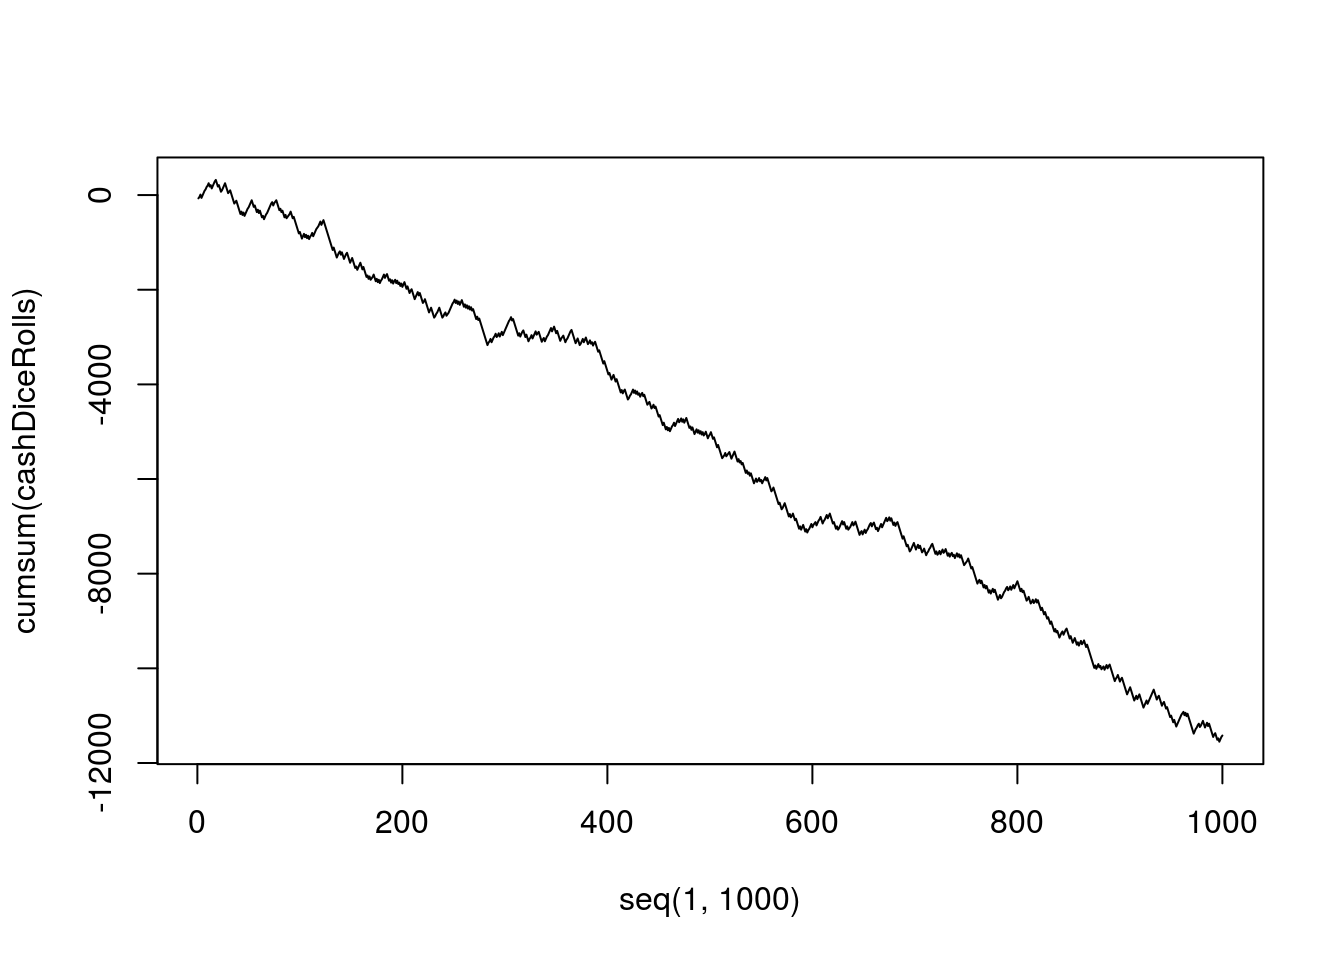
\includegraphics[width=0.6\linewidth]{BeginnersGuideToGalaxy_files/figure-latex/cassino-plot-1} 

}

\caption{How to lose cash in casino}\label{fig:cassino-plot}
\end{figure}

I think that your love to \textbf{R} is being deeper since I showed you
how it can save a lot of your money!

In nowadays stochastic analyses are more, and more popular. With
\textbf{R} it is quite easy to generate random numbers, sample and do
all the \emph{mumbo jumbo} on data. There are few functions that cover
\emph{classical} distributions: normal, Poisson, binomial, uniform (and
few others), that are actually build in base \textbf{R} distribution
(full list you will find
\href{https://stat.ethz.ch/R-manual/R-devel/library/stats/html/Distributions.html}{here}).
Some more sophisticated stuff is usually covered by some packages you
will need to download by yourself. You will easily find them by querying
Google like this
\href{https://www.google.com/search?client=ubuntu\&channel=fs\&q=Pearson+distribution+in+R\&ie=utf-8\&oe=utf-8\&gfe_rd=cr\&dcr=0\&ei=KTI5Ws_7LfPBXrSBr7gO}{Pearson
distribution in R}. By using this technique it is also possible to find
other useful packages for dealing with distributions (try to search for
package that allows you to sample from trimmed distribution). All the
distribution packages follow the same schema when naming functions. They
use letters: \texttt{d}, \texttt{p}, \texttt{q} and \texttt{r} followed
by abbreviation of distribution name to generate: density, distribution
function, quantile function and random numbers -- respectively. For
instance, lets generate ten random numbers from \emph{beta
distribution}, with parameters \texttt{10} and \texttt{3}:

\begin{Shaded}
\begin{Highlighting}[]
\KeywordTok{rbeta}\NormalTok{(}\DecValTok{25}\NormalTok{, }\DecValTok{10}\NormalTok{, }\DecValTok{3}\NormalTok{)}
\end{Highlighting}
\end{Shaded}

\begin{verbatim}
##  [1] 0.7759927 0.7562455 0.8347460 0.7973032 0.6406459 0.7331960 0.9008447
##  [8] 0.7302486 0.9039791 0.7724847 0.9335580 0.8189024 0.6804088 0.7402334
## [15] 0.6330118 0.7700679 0.8694151 0.5024869 0.7962756 0.7276797 0.6687331
## [22] 0.7571119 0.7947000 0.9254476 0.8096294
\end{verbatim}

Or we can make this nice plot (Fig. \ref{fig:betaDensity-plot}) for
density of \emph{beta distribution} with parameters \texttt{8} and
\texttt{3}:

\begin{figure}

{\centering 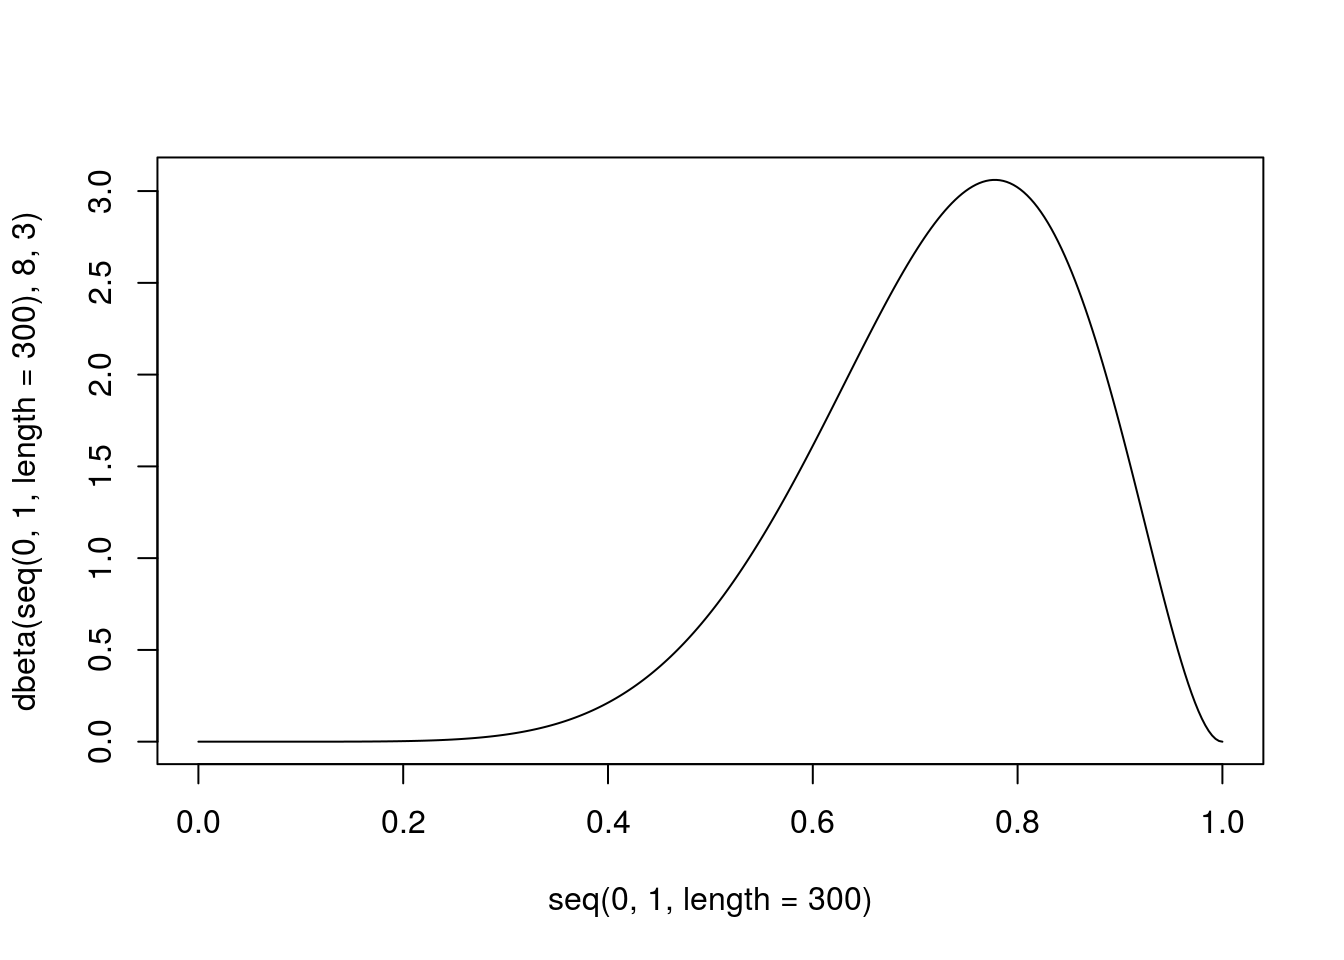
\includegraphics[width=0.6\linewidth]{BeginnersGuideToGalaxy_files/figure-latex/betaDensity-plot-1} 

}

\caption{Example of beta distribution}\label{fig:betaDensity-plot}
\end{figure}

\section{\texorpdfstring{\texttt{tidyverse} idea and \texttt{dplyr}
library}{tidyverse idea and dplyr library}}\label{tidyverse-idea-and-dplyr-library}

The whole idea of tidy data comes from one of most famous \textbf{R}
developers -- \href{http://hadley.nz/}{Hadley Wickham}. In on of his
papers \citep{hadley2014} he described procedures for generating and
cleaning data in standardized manner. Many packages right now are
designed to work best with data structured according to this
publication. Eventually it lead to \texttt{tidiverse} -- tools tailored
for data science with common syntax and philosophy \citep{R-tidyverse}.
One of the most useful packages that are included in \texttt{tidiverse}
\citep{R-tidyverse} are \texttt{tidyr} \citep{R-tidyr} and
\texttt{dplyr} \citep{R-dplyr}. First helps us to swap from `wide' to
`long' table format (and back). The second package contains set of tools
to easily manipulate rows, columns or even single cells in \emph{data
frame}. It is extremely powerful tool, which speeds up work with data
sets so much, that after few times dealing with it, you will leave
traditional spread sheet forever.

\subsection{Wide vs.~long tables}\label{wide-vs.long-tables}

Lets start with changing wide format table into long format table.

\begin{Shaded}
\begin{Highlighting}[]
\NormalTok{wideTable <-}\StringTok{ }\KeywordTok{data.frame}\NormalTok{(}\DataTypeTok{male =} \DecValTok{1}\OperatorTok{:}\DecValTok{10}\NormalTok{, }\DataTypeTok{female =} \DecValTok{3}\OperatorTok{:}\DecValTok{12}\NormalTok{)}
\NormalTok{wideTable}
\end{Highlighting}
\end{Shaded}

\begin{verbatim}
##    male female
## 1     1      3
## 2     2      4
## 3     3      5
## 4     4      6
## 5     5      7
## 6     6      8
## 7     7      9
## 8     8     10
## 9     9     11
## 10   10     12
\end{verbatim}

Than we just make a little \emph{mumbo jumbo} and change it to long
format:

\begin{Shaded}
\begin{Highlighting}[]
\KeywordTok{library}\NormalTok{(}\StringTok{'tidyr'}\NormalTok{)}
\KeywordTok{library}\NormalTok{(}\StringTok{'dplyr'}\NormalTok{)}
\NormalTok{longTable <-}\StringTok{ }\KeywordTok{gather}\NormalTok{(wideTable, }\DataTypeTok{key =}\NormalTok{ sex, }\DataTypeTok{value =}\NormalTok{ number)}
\NormalTok{longTable[}\DecValTok{7}\OperatorTok{:}\DecValTok{12}\NormalTok{, ]}
\end{Highlighting}
\end{Shaded}

\begin{verbatim}
##       sex number
## 7    male      7
## 8    male      8
## 9    male      9
## 10   male     10
## 11 female      3
## 12 female      4
\end{verbatim}

That is how easy it can be done. But what if table is more complicated?

\begin{Shaded}
\begin{Highlighting}[]
\NormalTok{wideTable2 <-}\StringTok{ }\KeywordTok{data.frame}\NormalTok{(}\DataTypeTok{male =} \DecValTok{1}\OperatorTok{:}\DecValTok{10}\NormalTok{,}
                         \DataTypeTok{female =} \DecValTok{3}\OperatorTok{:}\DecValTok{12}\NormalTok{, }
                         \DataTypeTok{type =} \KeywordTok{rep}\NormalTok{(}\KeywordTok{c}\NormalTok{(}\StringTok{'bacteria'}\NormalTok{, }\StringTok{'virus'}\NormalTok{), }\DataTypeTok{times =} \DecValTok{5}\NormalTok{),}
                         \DataTypeTok{group =} \KeywordTok{rep}\NormalTok{(}\KeywordTok{c}\NormalTok{(}\StringTok{'a'}\NormalTok{, }\StringTok{'b'}\NormalTok{), }\DataTypeTok{each =} \DecValTok{5}\NormalTok{))}
\NormalTok{wideTable2}
\end{Highlighting}
\end{Shaded}

\begin{verbatim}
##    male female     type group
## 1     1      3 bacteria     a
## 2     2      4    virus     a
## 3     3      5 bacteria     a
## 4     4      6    virus     a
## 5     5      7 bacteria     a
## 6     6      8    virus     b
## 7     7      9 bacteria     b
## 8     8     10    virus     b
## 9     9     11 bacteria     b
## 10   10     12    virus     b
\end{verbatim}

\begin{Shaded}
\begin{Highlighting}[]
\KeywordTok{gather}\NormalTok{(wideTable2, sex, number, }\OperatorTok{-}\KeywordTok{c}\NormalTok{(}\DecValTok{3}\NormalTok{, }\DecValTok{4}\NormalTok{))[}\DecValTok{7}\OperatorTok{:}\DecValTok{13}\NormalTok{, ]}
\end{Highlighting}
\end{Shaded}

\begin{verbatim}
##        type group    sex number
## 7  bacteria     b   male      7
## 8     virus     b   male      8
## 9  bacteria     b   male      9
## 10    virus     b   male     10
## 11 bacteria     a female      3
## 12    virus     a female      4
## 13 bacteria     a female      5
\end{verbatim}

In example above, using expression \texttt{-(3,\ 4)} we indicated that
we do not want to gather columns 3 and 4.

Even more complicated?

\begin{Shaded}
\begin{Highlighting}[]
\NormalTok{wideTable3 <-}\StringTok{ }\KeywordTok{data.frame}\NormalTok{(}\DataTypeTok{male =} \KeywordTok{rep}\NormalTok{(}\DecValTok{1}\OperatorTok{:}\DecValTok{10}\NormalTok{, }\DataTypeTok{each =} \DecValTok{2}\NormalTok{),}
                         \DataTypeTok{female =} \KeywordTok{rep}\NormalTok{(}\DecValTok{3}\OperatorTok{:}\DecValTok{12}\NormalTok{, }\DataTypeTok{times =} \DecValTok{2}\NormalTok{), }
                         \DataTypeTok{type =} \KeywordTok{rep}\NormalTok{(}\KeywordTok{c}\NormalTok{(}\StringTok{'bacteria'}\NormalTok{,}\StringTok{'virus'}\NormalTok{), }\DataTypeTok{times =} \DecValTok{10}\NormalTok{),}
                         \DataTypeTok{group =} \KeywordTok{rep}\NormalTok{(}\KeywordTok{c}\NormalTok{(}\StringTok{'a'}\NormalTok{,}\StringTok{'b'}\NormalTok{), }\DataTypeTok{each =} \DecValTok{10}\NormalTok{),}
                         \DataTypeTok{day =} \DecValTok{1}\OperatorTok{:}\DecValTok{10}\NormalTok{)}
\NormalTok{wideTable3[}\DecValTok{7}\OperatorTok{:}\DecValTok{13}\NormalTok{, ]}
\end{Highlighting}
\end{Shaded}

\begin{verbatim}
##    male female     type group day
## 7     4      9 bacteria     a   7
## 8     4     10    virus     a   8
## 9     5     11 bacteria     a   9
## 10    5     12    virus     a  10
## 11    6      3 bacteria     b   1
## 12    6      4    virus     b   2
## 13    7      5 bacteria     b   3
\end{verbatim}

\begin{Shaded}
\begin{Highlighting}[]
\KeywordTok{gather}\NormalTok{(wideTable3, sex, number, }\DecValTok{1}\OperatorTok{:}\DecValTok{2}\NormalTok{) }\OperatorTok
\StringTok{  }\KeywordTok{spread}\NormalTok{(group, number) }\OperatorTok\StringTok{ }\NormalTok{.[}\DecValTok{7}\OperatorTok{:}\DecValTok{13}\NormalTok{, ]}
\end{Highlighting}
\end{Shaded}

\begin{verbatim}
##        type day    sex  a  b
## 7  bacteria   7 female  9  9
## 8  bacteria   7   male  4  9
## 9  bacteria   9 female 11 11
## 10 bacteria   9   male  5 10
## 11    virus   2 female  4  4
## 12    virus   2   male  1  6
## 13    virus   4 female  6  6
\end{verbatim}

Here our data set had additional column \texttt{group} storing values
\texttt{a} and \texttt{b}. But imagine that \texttt{group} is not a
variable, but it just stores the names of variables - which are a and b.
This somehow might be frustrating, to decide if those are really
separate variables or not. You might run into problem, that your column
named \texttt{environmental\ factor} contains values: \emph{pH},
\emph{conductivity}, and \emph{oxygen concentration}. This would be
straightforward as each of this is different variable and you should
spread this column into three different variables. On the other hand you
might see a column that contains \emph{minimum temperature} and
\emph{maximum temperature}. This would not be as straightforward and
decision upon spreading this column would strongly depend on the
context. Nonetheless, using \texttt{spread()} function we were able to
transform values from this column as separate columns. We also used
\emph{piping operator} \texttt{\%\textgreater{}\%}. It is a shortcut,
which allows us to pass the left side as an argument to the function on
the right side of operator. In general it means that writing
\texttt{a\ \%\textgreater{}\%\ funtion(b)} actually is translated into
\texttt{function(a,\ b)}. In the beginning this idea might be not very
useful for you, but with time it will get helpful. Mainly because your
code gets better structure and you can perform multiple operations
without storing it in variables (which you do not want, since it
consumes memory).

There is also one more common case that I should shortly mention -
compound variable. It is a variable that stores multiple values in a
single column. E.g. city and district, age and sex, sex and smoking,
blood type and RH, etc. With \texttt{tidyr} is very easy to deal with
it.

\begin{Shaded}
\begin{Highlighting}[]
\NormalTok{wideTable4 <-}\StringTok{ }\KeywordTok{data.frame}\NormalTok{(}\DataTypeTok{type =} \KeywordTok{rep}\NormalTok{(}\KeywordTok{c}\NormalTok{(}\StringTok{'bacteria.a'}\NormalTok{, }\StringTok{'virus.a'}\NormalTok{), }\DataTypeTok{times =} \DecValTok{5}\NormalTok{))}
\NormalTok{wideTable4}
\end{Highlighting}
\end{Shaded}

\begin{verbatim}
##          type
## 1  bacteria.a
## 2     virus.a
## 3  bacteria.a
## 4     virus.a
## 5  bacteria.a
## 6     virus.a
## 7  bacteria.a
## 8     virus.a
## 9  bacteria.a
## 10    virus.a
\end{verbatim}

\begin{Shaded}
\begin{Highlighting}[]
\NormalTok{wideTable4 }\OperatorTok\StringTok{ }\KeywordTok{separate}\NormalTok{(type, }\KeywordTok{c}\NormalTok{(}\StringTok{'organism'}\NormalTok{, }\StringTok{'type'}\NormalTok{), }\DataTypeTok{sep =} \StringTok{'}\CharTok{\textbackslash{}\textbackslash{}}\StringTok{.'}\NormalTok{)}
\end{Highlighting}
\end{Shaded}

\begin{verbatim}
##    organism type
## 1  bacteria    a
## 2     virus    a
## 3  bacteria    a
## 4     virus    a
## 5  bacteria    a
## 6     virus    a
## 7  bacteria    a
## 8     virus    a
## 9  bacteria    a
## 10    virus    a
\end{verbatim}

\subsection{\texorpdfstring{World of
\texttt{dplyr}}{World of dplyr}}\label{world-of-dplyr}

\texttt{dplyr} is a library containing several useful functions,
designed to ease all kinds of transformations, selections and filtering
of your data frame. As the number and possibilities of functions are
really huge, here I will concentrate only on some mostly used ones. Of
course there is a well described documentation if you want to get
deeper.

\subsection{\texorpdfstring{\texttt{select} columns and \texttt{filter}
rows}{select columns and filter rows}}\label{select-columns-and-filter-rows}

Those are the most basic operations on \emph{data frames}.
\texttt{select()} function allows you to choose which columns you use.
The biggest advantage of using this function instead of simple
addressing, is that you can use some special functions inside it:
\texttt{starts\_with(),\ ends\_with(),\ contains(),\ matches(),\ num\_range()}
which are helpful when using large data sets with numerous columns.
There is also similar function \texttt{rename()} which can be used to
change variable names, but in results (contrary to \texttt{select()}) it
keeps all the variables. Lets look how the thing works on some simple
examples:

\begin{Shaded}
\begin{Highlighting}[]
\KeywordTok{head}\NormalTok{(}\KeywordTok{select}\NormalTok{(wideTable3, }\KeywordTok{starts_with}\NormalTok{(}\StringTok{'gr'}\NormalTok{)), }\DecValTok{3}\NormalTok{)}
\end{Highlighting}
\end{Shaded}

\begin{verbatim}
##   group
## 1     a
## 2     a
## 3     a
\end{verbatim}

\begin{Shaded}
\begin{Highlighting}[]
\KeywordTok{head}\NormalTok{(}\KeywordTok{select}\NormalTok{(wideTable3, }\OperatorTok{-}\KeywordTok{starts_with}\NormalTok{(}\StringTok{'gr'}\NormalTok{)), }\DecValTok{3}\NormalTok{)}
\end{Highlighting}
\end{Shaded}

\begin{verbatim}
##   male female     type day
## 1    1      3 bacteria   1
## 2    1      4    virus   2
## 3    2      5 bacteria   3
\end{verbatim}

\begin{Shaded}
\begin{Highlighting}[]
\KeywordTok{head}\NormalTok{(}\KeywordTok{select}\NormalTok{(wideTable3, }\KeywordTok{contains}\NormalTok{(}\StringTok{'ale'}\NormalTok{)), }\DecValTok{3}\NormalTok{)}
\end{Highlighting}
\end{Shaded}

\begin{verbatim}
##   male female
## 1    1      3
## 2    1      4
## 3    2      5
\end{verbatim}

\begin{Shaded}
\begin{Highlighting}[]
\KeywordTok{head}\NormalTok{(}\KeywordTok{rename}\NormalTok{(wideTable3, }\DataTypeTok{Male =}\NormalTok{ male), }\DecValTok{3}\NormalTok{)}
\end{Highlighting}
\end{Shaded}

\begin{verbatim}
##   Male female     type group day
## 1    1      3 bacteria     a   1
## 2    1      4    virus     a   2
## 3    2      5 bacteria     a   3
\end{verbatim}

Filtering rows is also straightforward. Inside function
\texttt{filter()} you can use logical operators
(\texttt{\&,\ \textbar{},\ xor,\ !}), comparisons (e.g. \texttt{==} or
\texttt{\textgreater{}=}), or functions
(\texttt{is.na(),\ between(),\ near()}).

\begin{Shaded}
\begin{Highlighting}[]
\KeywordTok{filter}\NormalTok{(wideTable3, group }\OperatorTok{==}\StringTok{ 'a'}\NormalTok{)}
\end{Highlighting}
\end{Shaded}

\begin{verbatim}
##    male female     type group day
## 1     1      3 bacteria     a   1
## 2     1      4    virus     a   2
## 3     2      5 bacteria     a   3
## 4     2      6    virus     a   4
## 5     3      7 bacteria     a   5
## 6     3      8    virus     a   6
## 7     4      9 bacteria     a   7
## 8     4     10    virus     a   8
## 9     5     11 bacteria     a   9
## 10    5     12    virus     a  10
\end{verbatim}

\begin{Shaded}
\begin{Highlighting}[]
\KeywordTok{filter}\NormalTok{(wideTable3, type }\OperatorTok{!=}\StringTok{ 'bacteria'}\NormalTok{)}
\end{Highlighting}
\end{Shaded}

\begin{verbatim}
##    male female  type group day
## 1     1      4 virus     a   2
## 2     2      6 virus     a   4
## 3     3      8 virus     a   6
## 4     4     10 virus     a   8
## 5     5     12 virus     a  10
## 6     6      4 virus     b   2
## 7     7      6 virus     b   4
## 8     8      8 virus     b   6
## 9     9     10 virus     b   8
## 10   10     12 virus     b  10
\end{verbatim}

\begin{Shaded}
\begin{Highlighting}[]
\KeywordTok{filter}\NormalTok{(wideTable3, }\KeywordTok{near}\NormalTok{(female, }\DecValTok{5}\NormalTok{))}
\end{Highlighting}
\end{Shaded}

\begin{verbatim}
##   male female     type group day
## 1    2      5 bacteria     a   3
## 2    7      5 bacteria     b   3
\end{verbatim}

\subsection{\texorpdfstring{\texttt{mutate} and
\texttt{transmute}}{mutate and transmute}}\label{mutate-and-transmute}

Both functions are widely used in data manipulation in \textbf{R}. Their
main purpose is to create new variable (usually from existing ones) in
data frame. Lets look on examples:

\begin{Shaded}
\begin{Highlighting}[]
\KeywordTok{select}\NormalTok{(wideTable3, male) }\OperatorTok
\StringTok{  }\KeywordTok{mutate}\NormalTok{(}\DataTypeTok{cumulativeMaleSum =} \KeywordTok{cumsum}\NormalTok{(male)) }\OperatorTok
\StringTok{  }\KeywordTok{head}\NormalTok{(}\DecValTok{5}\NormalTok{)}
\end{Highlighting}
\end{Shaded}

\begin{verbatim}
##   male cumulativeMaleSum
## 1    1                 1
## 2    1                 2
## 3    2                 4
## 4    2                 6
## 5    3                 9
\end{verbatim}

\begin{Shaded}
\begin{Highlighting}[]
\KeywordTok{select}\NormalTok{(wideTable3, male, female) }\OperatorTok
\StringTok{  }\KeywordTok{mutate}\NormalTok{(}\DataTypeTok{cumulativeMaleSum =} \KeywordTok{cumsum}\NormalTok{(male),}
         \DataTypeTok{femaleLog =} \KeywordTok{log}\NormalTok{(female),}
         \DataTypeTok{cumSumFemaleLog =} \KeywordTok{cumsum}\NormalTok{(femaleLog)) }\OperatorTok
\StringTok{  }\KeywordTok{head}\NormalTok{(}\DecValTok{5}\NormalTok{)}
\end{Highlighting}
\end{Shaded}

\begin{verbatim}
##   male female cumulativeMaleSum femaleLog cumSumFemaleLog
## 1    1      3                 1  1.098612        1.098612
## 2    1      4                 2  1.386294        2.484907
## 3    2      5                 4  1.609438        4.094345
## 4    2      6                 6  1.791759        5.886104
## 5    3      7                 9  1.945910        7.832014
\end{verbatim}

As you can see in second example, when we use \texttt{mutate()}
function, the newly created variables (in this example
\texttt{femaleLog}) are available immediately so we can use them to
create another variable (in this case \texttt{cumSumFemaleLog}) within
one function call. In this example, I also used piping operator, because
calculating intermediate steps and storing them as a result, which can
be used later is useless, as we are interested only in the final
outcome. The biggest advantage of this procedure is that we keep our
\emph{Environment} clean and preserve memory -- which is very important
in long and memory consuming projects. Last but not least, the
difference between \texttt{mutate()} and \texttt{transmute()} is that
the latter do not preserve all variables, only the ones you created.

\subsection{\texorpdfstring{\texttt{group\_by} and
\texttt{summarise}}{group\_by and summarise}}\label{group_by-and-summarise}

\texttt{summarise()} is commonly used function on grouped data. It
allows to calculate many typical descriptive statistics (like
\texttt{mean()} or \texttt{quantile()}) for particular groups in you
data set, as well as it can count number of observations (\texttt{n()}
function), or number of unique observations (\texttt{distinct()}). To
see how it works in practice lets look back on our example and calculate
mean value for \texttt{males} and \texttt{female}, as well as day range
and number of cases for groups derived from \texttt{type}.

\begin{Shaded}
\begin{Highlighting}[]
\NormalTok{wideTable3 }\OperatorTok\StringTok{ }
\StringTok{  }\KeywordTok{group_by}\NormalTok{(type) }\OperatorTok\StringTok{ }
\StringTok{  }\KeywordTok{summarise}\NormalTok{(}\DataTypeTok{meanF =} \KeywordTok{mean}\NormalTok{(female),}
            \DataTypeTok{meanM =} \KeywordTok{mean}\NormalTok{(male),}
            \DataTypeTok{numberOfDays =}\NormalTok{ (}\KeywordTok{range}\NormalTok{(day)[}\DecValTok{2}\NormalTok{]}\OperatorTok{-}\KeywordTok{range}\NormalTok{(day)[}\DecValTok{1}\NormalTok{]),}
            \DataTypeTok{numberOfCases =} \KeywordTok{n}\NormalTok{())}
\end{Highlighting}
\end{Shaded}

\begin{verbatim}
## # A tibble: 2 x 5
##   type     meanF meanM numberOfDays numberOfCases
##   <fct>    <dbl> <dbl>        <int>         <int>
## 1 bacteria    7.  5.50            8            10
## 2 virus       8.  5.50            8            10
\end{verbatim}

Easy.

\section{\texorpdfstring{Is there anything more in \texttt{dplyr}
library?}{Is there anything more in dplyr library?}}\label{is-there-anything-more-in-dplyr-library}

Yes. Actually I presented here only very very tiny fracture of
\texttt{dplyr} possibilities just to familiarize you with syntax and
using piping operator. When you go deeper into world of data frames
transformation, you will find other commonly used functions like:
different kinds of joining data frames (similar to \textbf{SQL} joining
tables), conditional selecting, filtering, renaming rows and columns,
extracting values or arranging your data frame. Thankfully this
procedures are so common that even if you won't grasp it immediately
from functions description, you will still find hundreds of tutorials on
the web, or help in \emph{StackOverflow}.

\chapter{Lets do some math!}\label{lets-do-some-math}

\section{Models}\label{models}

\begin{center}\rule{0.5\linewidth}{\linethickness}\end{center}

\begin{center}
\begingroup\Large
Simple statistical model  
\endgroup
\end{center}

\begin{center}\rule{0.5\linewidth}{\linethickness}\end{center}

OK. There is no such thing as simple statistical model. However there
are lots of packages that will make you suffer less. In fact this is one
of biggest \textbf{R} advantages, that you can make even very
sophisticated statistical modelling without any knowledge on programming
since you use \emph{black boxes}. When you are dealing with classic
statistical models many of them are included in \textbf{base R}
distribution -- like linear or generalized additive models. You probably
need to use mixed effect models, at some point. Good news is that there
is a very nice and quite straightforward to use package called
\texttt{lme4}. Every time you run into problem, and you do not know what
to use for statistical modelling, or how to perform full procedure, just
query Google. There are hundreds of blogs, web pages and \emph{Stack
Overflow} discussion on it.

\begin{center}\rule{0.5\linewidth}{\linethickness}\end{center}

\begin{center}
\begingroup\Large*
Other models  
\endgroup
\end{center}

\begin{center}\rule{0.5\linewidth}{\linethickness}\end{center}

Besides \emph{simple statistical models}, there is a lot of other
models. The scope of this book is not to discuss dichotomies in
classification of models. To keep things simple, we will just stick to
\emph{models} that can be described with at least one of the following
adjectives: \emph{stochastic}, \emph{mechanistic} or belong to
\emph{differential equations systems}.

\section{Packages}\label{packages}

Other, usually dynamic models, require more knowledge, experience and
some packages. Before you start looking for more tailored solutions,
install following packages: \texttt{deSolve}, \texttt{fitdistrplus},
\texttt{rriskDistributions} and \texttt{truncdist}. First one contains
tools for solving differential equations sets, second and third provides
you tools to deal with distributions (such as comparing distributions or
estimating its parameters), and the last one allows you to use truncated
distributions.

\section{Simple mechanistic model and
noise}\label{simple-mechanistic-model-and-noise}

To show some basic mechanistic model, we will use the well known
Michaelis-Menten function: \(f(x) = \frac{ax}{b+x}\), with
\emph{parameter a = 2.15} and \emph{parameter b = 0.08}.

\begin{Shaded}
\begin{Highlighting}[]
\NormalTok{parA <-}\StringTok{ }\FloatTok{2.15}
\NormalTok{parB <-}\StringTok{ }\FloatTok{0.08}
\NormalTok{varX <-}\StringTok{ }\KeywordTok{seq}\NormalTok{(}\DecValTok{0}\NormalTok{,}\DecValTok{1}\NormalTok{, }\DataTypeTok{length.out =} \DecValTok{1000}\NormalTok{)}
\NormalTok{mmFunction <-}\StringTok{ }\NormalTok{parA }\OperatorTok{*}\StringTok{ }\NormalTok{varX}\OperatorTok{/}\NormalTok{(parB }\OperatorTok{+}\StringTok{ }\NormalTok{varX)}
\KeywordTok{plot}\NormalTok{(mmFunction}\OperatorTok{~}\NormalTok{varX, }\DataTypeTok{type =} \StringTok{'l'}\NormalTok{)}
\end{Highlighting}
\end{Shaded}

\begin{figure}
\centering
\includegraphics{BeginnersGuideToGalaxy_files/figure-latex/MMfunction-1.pdf}
\caption{\label{fig:MMfunction}Simple Michaelis-Menten function}
\end{figure}

As you can see, as long as you have simple equation it is very
straightforward to translate it into R. But we want something more
useful, for instance adding noise or uncertainty to our model. Lets
assume, that we are not sure what is the value of \emph{parameter a}.
Lets say that from previous research and expert knowledge we assume that
it can be as high 2.5, but never is lower than 1.8. Also it usually
takes value of 2.15. Knowing this we can use PERT distribution to
include uncertainty in model.

\begin{Shaded}
\begin{Highlighting}[]
\KeywordTok{library}\NormalTok{(}\StringTok{'mc2d'}\NormalTok{)}
\NormalTok{sParA <-}\StringTok{ }\KeywordTok{rpert}\NormalTok{(}\DecValTok{1000}\NormalTok{, }\FloatTok{1.8}\NormalTok{, }\FloatTok{2.15}\NormalTok{, }\FloatTok{2.5}\NormalTok{)}
\NormalTok{parB <-}\StringTok{ }\FloatTok{0.08}
\NormalTok{mmSAFunction <-}\StringTok{ }\NormalTok{sParA }\OperatorTok{*}\StringTok{ }\NormalTok{varX}\OperatorTok{/}\NormalTok{(parB }\OperatorTok{+}\StringTok{ }\NormalTok{varX)}
\end{Highlighting}
\end{Shaded}

We added some uncertainty to our function. But what with \emph{parameter
b}, how our uncertainty on its value affects the outcome? Lets assume
that it's value is normally distributed with \emph{mean = 0.8} and
\emph{sd = 0.23}.

\begin{Shaded}
\begin{Highlighting}[]
\NormalTok{sParB <-}\StringTok{ }\KeywordTok{rnorm}\NormalTok{(}\DecValTok{1000}\NormalTok{, }\FloatTok{0.08}\NormalTok{, }\FloatTok{0.023}\NormalTok{) }
\NormalTok{mmSABFunction <-}\StringTok{ }\NormalTok{sParA }\OperatorTok{*}\StringTok{ }\NormalTok{varX}\OperatorTok{/}\NormalTok{(sParB }\OperatorTok{+}\StringTok{ }\NormalTok{varX)}
\end{Highlighting}
\end{Shaded}

Let me put this two functions on plots side by side:

\begin{Shaded}
\begin{Highlighting}[]
\KeywordTok{par}\NormalTok{(}\DataTypeTok{mfrow =} \KeywordTok{c}\NormalTok{(}\DecValTok{1}\NormalTok{,}\DecValTok{2}\NormalTok{))}
\KeywordTok{plot}\NormalTok{(mmSAFunction}\OperatorTok{~}\NormalTok{varX, }\DataTypeTok{type =} \StringTok{'l'}\NormalTok{)}
\KeywordTok{plot}\NormalTok{(mmSABFunction}\OperatorTok{~}\NormalTok{varX, }\DataTypeTok{type =} \StringTok{'l'}\NormalTok{)}
\KeywordTok{par}\NormalTok{(}\DataTypeTok{mfrow =} \KeywordTok{c}\NormalTok{(}\DecValTok{1}\NormalTok{,}\DecValTok{1}\NormalTok{))}
\end{Highlighting}
\end{Shaded}

\begin{figure}
\centering
\includegraphics{BeginnersGuideToGalaxy_files/figure-latex/MMfunctionAB-1.pdf}
\caption{\label{fig:MMfunctionAB}Michaelis-Menten function with stochastic
parameter A (left) or A and B (right)}
\end{figure}

It seems that inclusion of uncertainty on value of \emph{parameter b}
does change our outcome. Lets also include some variability into the
outcome. We can assume that for some reasons value of function will vary
more than just our uncertainty about value of both \emph{parameters}.
And usually it varies from \(f(x)\) by some value from uniform
distribution. The 25\textsuperscript{th} and 75\textsuperscript{th}
percentile are given by: \texttt{-0.13} and \texttt{0.17}. To calculate
parameters of this distribution we will use \texttt{rriskDistributions}
package.

\begin{Shaded}
\begin{Highlighting}[]
\KeywordTok{library}\NormalTok{(}\StringTok{'rriskDistributions'}\NormalTok{)}
\NormalTok{unifParams <-}\StringTok{ }\KeywordTok{get.unif.par}\NormalTok{(}\DataTypeTok{p =} \KeywordTok{c}\NormalTok{(}\FloatTok{0.25}\NormalTok{, }\FloatTok{0.75}\NormalTok{), }\DataTypeTok{q =} \KeywordTok{c}\NormalTok{(}\OperatorTok{-}\FloatTok{0.13}\NormalTok{, }\FloatTok{0.17}\NormalTok{), }\DataTypeTok{plot =}\NormalTok{ F)}
\NormalTok{fVariability <-}\StringTok{ }\KeywordTok{runif}\NormalTok{(}\DecValTok{1000}\NormalTok{, }\DataTypeTok{min =}\NormalTok{ unifParams[}\DecValTok{1}\NormalTok{], }\DataTypeTok{max =}\NormalTok{ unifParams[}\DecValTok{2}\NormalTok{])}
\NormalTok{mmFSFunction <-}\StringTok{ }\NormalTok{((sParA }\OperatorTok{*}\StringTok{ }\NormalTok{varX}\OperatorTok{/}\NormalTok{(sParB }\OperatorTok{+}\StringTok{ }\NormalTok{varX)) }\OperatorTok{+}\StringTok{ }\NormalTok{fVariability)}
\KeywordTok{plot}\NormalTok{(mmFSFunction}\OperatorTok{~}\NormalTok{varX, }\DataTypeTok{type =} \StringTok{'l'}\NormalTok{)}
\end{Highlighting}
\end{Shaded}

\begin{figure}
\centering
\includegraphics{BeginnersGuideToGalaxy_files/figure-latex/unnamed-chunk-44-1.pdf}
\caption{\label{fig:unnamed-chunk-44}Michaelis-Menten function fully
stochastic}
\end{figure}

It seems that there are differences between those three plots. So lets
overlay them one on another to inspect visually differences.

\begin{Shaded}
\begin{Highlighting}[]
\KeywordTok{plot}\NormalTok{(varX, mmFunction, }\DataTypeTok{type =} \StringTok{'l'}\NormalTok{,}
     \DataTypeTok{col =} \StringTok{'black'}\NormalTok{, }\DataTypeTok{ylim =} \KeywordTok{c}\NormalTok{(}\DecValTok{0}\NormalTok{, }\DecValTok{3}\NormalTok{),}
     \DataTypeTok{main =} \StringTok{'Michaelis-Menten function'}\NormalTok{, }\DataTypeTok{xlab =} \StringTok{'x'}\NormalTok{, }\DataTypeTok{ylab =} \StringTok{'f(x) = a*x/(b+x)'}\NormalTok{)}
\KeywordTok{lines}\NormalTok{(varX, mmSAFunction, }\DataTypeTok{col =} \StringTok{'blue'}\NormalTok{)}
\KeywordTok{lines}\NormalTok{(varX, mmSABFunction, }\DataTypeTok{col =} \StringTok{'green'}\NormalTok{, }\DataTypeTok{lty =} \StringTok{'dashed'}\NormalTok{)}
\KeywordTok{lines}\NormalTok{(varX, mmFSFunction, }\DataTypeTok{col =} \StringTok{'red'}\NormalTok{, }\DataTypeTok{lty =} \StringTok{'dotted'}\NormalTok{)}
\end{Highlighting}
\end{Shaded}

\begin{figure}
\centering
\includegraphics{BeginnersGuideToGalaxy_files/figure-latex/unnamed-chunk-45-1.pdf}
\caption{\label{fig:unnamed-chunk-45}Michaelis-Menten function with
different levels of stochasticity}
\end{figure}

\section{Solving differential
equations}\label{solving-differential-equations}

\subsection{The simple
epidemiological}\label{the-simple-epidemiological}

SIR (Susceptible, Infectious, Recovered) is a typical compartmental
model for epidemiology. Since it has only 3 compartments, it is hard to
find an easier one to model with differential equations. In our example
we will use slightly more complicated example with four compartments --
SEIR (Susceptible, Exposed, Infectious, Recovered). We begin with
defining parameters of initial population. We need to define: birth and
death rate, transmission (\(\beta\)), \(\gamma\) (\(\frac{1}{\gamma}\)
defines infectious period) and \(\alpha\) (\(\frac{1}{\alpha}\) defines
latent period). Than we define time and initial conditions -- number of
all specimens, population size, number of exposed, number of initially
infected, number of initially recovered, which we combine in
\texttt{initial} values vector.\\
Main step of this procedure is to define function which will be used to
solve \emph{Ordinary Differential Equations (ODE)}. This function takes
three parameter -- t (which is time sequence), state (which are our
initial conditions) and parameters. In the body of the function we
define differential equations which connect our compartments. To solve
the system of differential equations we use \texttt{ode()} function from
\texttt{deSolve} package and save our results in \texttt{modelOutput}
variable, which we will later use to make a plot.

\begin{Shaded}
\begin{Highlighting}[]
\NormalTok{parameters <-}\StringTok{ }\KeywordTok{c}\NormalTok{(}\DataTypeTok{b     =} \FloatTok{0.1}\NormalTok{,        }\CommentTok{# birth rate}
                \DataTypeTok{d     =} \FloatTok{0.1}\NormalTok{,        }\CommentTok{# death rate}
                \DataTypeTok{beta  =} \FloatTok{0.00025}\NormalTok{,    }\CommentTok{# transmission parameter}
                \DataTypeTok{gamma =} \FloatTok{0.6}\NormalTok{,        }\CommentTok{# 1/gamma = infectious period}
                \DataTypeTok{a     =} \FloatTok{0.1}        \CommentTok{# 1/a = latent period}
\NormalTok{                )}

\NormalTok{time <-}\StringTok{ }\DecValTok{1}\OperatorTok{:}\DecValTok{100}

\CommentTok{# Initial conditions}
\NormalTok{N =}\StringTok{ }\DecValTok{15000}    \CommentTok{# population size}
\NormalTok{E0 =}\StringTok{ }\DecValTok{150}     \CommentTok{# initialy exposed}
\NormalTok{I0 =}\StringTok{ }\DecValTok{15}      \CommentTok{# initialy infected}
\NormalTok{R0 =}\StringTok{ }\DecValTok{20}      \CommentTok{# initialy recovered}

\NormalTok{initial <-}\StringTok{ }\KeywordTok{c}\NormalTok{(}\DataTypeTok{S =}\NormalTok{ N }\OperatorTok{-}\StringTok{ }\NormalTok{(E0 }\OperatorTok{+}\StringTok{ }\NormalTok{I0 }\OperatorTok{+}\StringTok{ }\NormalTok{R0), }\DataTypeTok{E =}\NormalTok{ E0, }\DataTypeTok{I=}\NormalTok{ I0, }\DataTypeTok{R =}\NormalTok{ R0)}

\CommentTok{# ODE Model}
\NormalTok{fSEIR <-}\StringTok{ }\ControlFlowTok{function}\NormalTok{(t, state, parameters) \{}
  \KeywordTok{with}\NormalTok{(}\KeywordTok{as.list}\NormalTok{(}\KeywordTok{c}\NormalTok{(state, parameters)), \{}
\NormalTok{    dS =}\StringTok{ }\NormalTok{b }\OperatorTok{*}\StringTok{ }\NormalTok{(S }\OperatorTok{+}\StringTok{ }\NormalTok{E }\OperatorTok{+}\StringTok{ }\NormalTok{I }\OperatorTok{+}\StringTok{ }\NormalTok{R) }\OperatorTok{-}\StringTok{ }\NormalTok{beta }\OperatorTok{*}\StringTok{ }\NormalTok{S }\OperatorTok{*}\StringTok{ }\NormalTok{I }\OperatorTok{-}\StringTok{ }\NormalTok{d }\OperatorTok{*}\StringTok{ }\NormalTok{S}
\NormalTok{    dE =}\StringTok{ }\NormalTok{beta }\OperatorTok{*}\StringTok{ }\NormalTok{S }\OperatorTok{*}\StringTok{ }\NormalTok{I }\OperatorTok{-}\StringTok{ }\NormalTok{a }\OperatorTok{*}\StringTok{ }\NormalTok{E }\OperatorTok{-}\StringTok{ }\NormalTok{d }\OperatorTok{*}\StringTok{ }\NormalTok{E}
\NormalTok{    dI =}\StringTok{ }\NormalTok{a }\OperatorTok{*}\StringTok{ }\NormalTok{E }\OperatorTok{-}\StringTok{ }\NormalTok{gamma }\OperatorTok{*}\StringTok{ }\NormalTok{I }\OperatorTok{-}\StringTok{ }\NormalTok{d }\OperatorTok{*}\StringTok{ }\NormalTok{I}
\NormalTok{    dR =}\StringTok{ }\NormalTok{gamma }\OperatorTok{*}\StringTok{ }\NormalTok{I }\OperatorTok{-}\StringTok{ }\NormalTok{d }\OperatorTok{*}\StringTok{ }\NormalTok{R}
    \KeywordTok{return}\NormalTok{(}\KeywordTok{list}\NormalTok{(}\KeywordTok{c}\NormalTok{(dS, dE, dI, dR)))}
\NormalTok{  \})}
\NormalTok{\}}

\NormalTok{modelOutput <-}\StringTok{ }\NormalTok{deSolve}\OperatorTok{::}\KeywordTok{ode}\NormalTok{(}\DataTypeTok{y =}\NormalTok{ initial, }\DataTypeTok{func =}\NormalTok{ fSEIR, }\DataTypeTok{times =}\NormalTok{ time, }\DataTypeTok{parms =}\NormalTok{ parameters)}
\KeywordTok{head}\NormalTok{(modelOutput)}
\end{Highlighting}
\end{Shaded}

\begin{verbatim}
##      time        S        E        I        R
## [1,]    1 14815.00 150.0000 15.00000 20.00000
## [2,]    2 14771.93 180.7236 19.41006 27.94129
## [3,]    3 14717.22 220.8724 24.19132 37.72072
## [4,]    4 14649.90 270.7314 29.83648 49.53296
## [5,]    5 14567.85 331.7169 36.66138 63.77320
## [6,]    6 14468.27 405.8173 44.94943 80.96618
\end{verbatim}

\subsection{Ploting SERI model}\label{ploting-seri-model}

To create a plot using our favorite library \texttt{ggplot2} (which will
be described with more details in chapter \ref{graphs}) we first need to
convert our modelOutput to object of class \emph{data frame}. Than we
can use code below to plot our model.

\begin{Shaded}
\begin{Highlighting}[]
\NormalTok{modelOutput <-}\StringTok{ }\KeywordTok{as.data.frame}\NormalTok{(modelOutput)}
\KeywordTok{ggplot}\NormalTok{(modelOutput, }\KeywordTok{aes}\NormalTok{(}\DataTypeTok{x =}\NormalTok{ time)) }\OperatorTok{+}
\StringTok{  }\KeywordTok{geom_line}\NormalTok{(}\KeywordTok{aes}\NormalTok{(}\DataTypeTok{y =}\NormalTok{ S, }\DataTypeTok{colour =} \StringTok{"S"}\NormalTok{)) }\OperatorTok{+}\StringTok{ }
\StringTok{  }\KeywordTok{geom_line}\NormalTok{(}\KeywordTok{aes}\NormalTok{(}\DataTypeTok{y =}\NormalTok{ E, }\DataTypeTok{colour =} \StringTok{"E"}\NormalTok{)) }\OperatorTok{+}
\StringTok{  }\KeywordTok{geom_line}\NormalTok{(}\KeywordTok{aes}\NormalTok{(}\DataTypeTok{y =}\NormalTok{ I, }\DataTypeTok{colour =} \StringTok{"I"}\NormalTok{)) }\OperatorTok{+}\StringTok{ }
\StringTok{  }\KeywordTok{geom_line}\NormalTok{(}\KeywordTok{aes}\NormalTok{(}\DataTypeTok{y =}\NormalTok{ R, }\DataTypeTok{colour =} \StringTok{"R"}\NormalTok{))}
\end{Highlighting}
\end{Shaded}

\includegraphics{BeginnersGuideToGalaxy_files/figure-latex/unnamed-chunk-47-1.pdf}

However, the element \texttt{geom\_line} is repeated four times, which
does not look nice. We can change it with little effort, and also define
some better aesthetics:

\begin{Shaded}
\begin{Highlighting}[]
\NormalTok{modelOutput <-}\StringTok{ }\KeywordTok{as.data.frame}\NormalTok{(modelOutput) }\OperatorTok
\StringTok{  }\KeywordTok{gather}\NormalTok{(}\DataTypeTok{key =}\NormalTok{ compartment, }\DataTypeTok{value =}\NormalTok{ value, }\OperatorTok{-}\NormalTok{time) }\OperatorTok
\StringTok{  }\KeywordTok{left_join}\NormalTok{(}\KeywordTok{data.frame}\NormalTok{(}\DataTypeTok{compartment =} \KeywordTok{c}\NormalTok{(}\StringTok{"S"}\NormalTok{, }\StringTok{"E"}\NormalTok{, }\StringTok{"I"}\NormalTok{, }\StringTok{"R"}\NormalTok{),}
                       \DataTypeTok{ordered =} \DecValTok{1}\OperatorTok{:}\DecValTok{4}\NormalTok{,}
                       \DataTypeTok{stringsAsFactors =}\NormalTok{ F), }\DataTypeTok{by =} \StringTok{'compartment'}\NormalTok{)}
\KeywordTok{ggplot}\NormalTok{(modelOutput, }\KeywordTok{aes}\NormalTok{(}\DataTypeTok{x =}\NormalTok{ time, }\DataTypeTok{y =}\NormalTok{ value,}
                        \DataTypeTok{colour =} \KeywordTok{reorder}\NormalTok{(compartment, ordered))) }\OperatorTok{+}
\StringTok{  }\KeywordTok{geom_line}\NormalTok{() }\OperatorTok{+}
\StringTok{  }\NormalTok{viridis}\OperatorTok{::}\KeywordTok{scale_colour_viridis}\NormalTok{(}\DataTypeTok{discrete =}\NormalTok{ T) }\OperatorTok{+}
\StringTok{  }\KeywordTok{theme_bw}\NormalTok{() }\OperatorTok{+}
\StringTok{  }\KeywordTok{theme}\NormalTok{(}\DataTypeTok{panel.grid.major.y =} \KeywordTok{element_line}\NormalTok{(}\DataTypeTok{colour =} \StringTok{"#dfdfdf"}\NormalTok{)) }\OperatorTok{+}
\StringTok{  }\KeywordTok{labs}\NormalTok{(}\DataTypeTok{colour =} \StringTok{'Compartment'}\NormalTok{,}
       \DataTypeTok{x =} \StringTok{'Time'}\NormalTok{,}
       \DataTypeTok{y =} \StringTok{'Population size'}\NormalTok{,}
       \DataTypeTok{title =} \StringTok{'SERI epidemiological model'}\NormalTok{)}
\end{Highlighting}
\end{Shaded}

\includegraphics{BeginnersGuideToGalaxy_files/figure-latex/unnamed-chunk-48-1.pdf}

You might wonder why we added additional column to \texttt{modelOutput}
data frame. The thing is that \texttt{ggplot} automatically maps some
aesthetics to groups using alphabetical order. Created column in which
we store numbers that refer to compartment order in \emph{SERI} acronym.
Than we use it as argument to \texttt{reorder} function inside
\texttt{ggplot}, which under the hood transforms variable to
\emph{factor} and change \emph{level} orders. Using this approach, we
don't need to change all the orderings of variables and aesthetics
manually. I also used color palette from *\texttt{viridis} package,
which contains four nice looking color palettes, which are colorblind
safe (at least in theory).

\chapter{Functions}\label{finalindications}

In short, function is a piece of code that takes some arguments, makes
\emph{mumbo jumbo} and returns result. All the time, through this book
we were using functions that are built in \textbf{base R} or comes from
additional packages (like \texttt{dplyr}). So you are now quite familiar
whit the syntax that resembles typical mathematical syntax -- \emph{name
of a function followed by arguments in brackets - like f(x)}. From time
to time you will need to do something in your code for few times with
different arguments. In order to not repeat yourself and not \emph{copy
-- paste} your code multiple times you can wrap your procedure in a
function. The best way (as always) to understand how to do it, is to do
it. To begin with something simple we will start with making basic math
functions which later will lead us to simple calculator.

\section{Simple math functions.}\label{simple-math-functions.}

Simple math operations include: \emph{adding}, \emph{substracting},
\emph{dividing} and \emph{multipling}. To make our calculator slightly
less boring, we can also add \emph{powers} and \emph{nth rooting}. To
not to complicate to much things in the beginning, lets say that we want
our function to take two and only two arguments. Lets look below how to
code our functions:

\begin{Shaded}
\begin{Highlighting}[]
\NormalTok{addF <-}\StringTok{ }\ControlFlowTok{function}\NormalTok{(x,y) \{}
  \KeywordTok{return}\NormalTok{(x}\OperatorTok{+}\NormalTok{y)}
\NormalTok{\}}
\NormalTok{subF <-}\StringTok{ }\ControlFlowTok{function}\NormalTok{(x,y) \{}
  \KeywordTok{return}\NormalTok{(x}\OperatorTok{-}\NormalTok{y)}
\NormalTok{\}}
\NormalTok{divF <-}\StringTok{ }\ControlFlowTok{function}\NormalTok{(x,y) \{}
  \KeywordTok{return}\NormalTok{(x}\OperatorTok{/}\NormalTok{y)}
\NormalTok{\}}
\NormalTok{mulF <-}\StringTok{ }\ControlFlowTok{function}\NormalTok{(x,y) \{}
  \KeywordTok{return}\NormalTok{(x}\OperatorTok{*}\NormalTok{y)}
\NormalTok{\}}
\NormalTok{powF <-}\StringTok{ }\ControlFlowTok{function}\NormalTok{(x,y) \{}
  \KeywordTok{return}\NormalTok{(x}\OperatorTok{:}\NormalTok{y)}
\NormalTok{\}}
\NormalTok{ntrF <-}\StringTok{ }\ControlFlowTok{function}\NormalTok{(x,y) \{}
  \KeywordTok{return}\NormalTok{(x}\OperatorTok{^}\NormalTok{(}\DecValTok{1}\OperatorTok{/}\NormalTok{y))}
\NormalTok{\}}
\end{Highlighting}
\end{Shaded}

\section{Building your own
calculator}\label{building-your-own-calculator}

Above example is of course useless and boring. So lets quickly get to
making calculator, that would use one of above functions, or return
results of all of them. So actually this time we will make so called
\emph{wraper} around previously made functions. We will use
\emph{switch} functionality, so besides our two parameters: \texttt{x}
and \texttt{y} we will also tell our function which of the results we
are interested in.

\begin{Shaded}
\begin{Highlighting}[]
\NormalTok{simpleCalculator <-}\StringTok{ }\ControlFlowTok{function}\NormalTok{(x, y, mathType) \{}
\NormalTok{  addF <-}\StringTok{ }\ControlFlowTok{function}\NormalTok{(x, y) \{}
  \KeywordTok{return}\NormalTok{(x}\OperatorTok{+}\NormalTok{y)}
\NormalTok{  \}}
\NormalTok{  subF <-}\StringTok{ }\ControlFlowTok{function}\NormalTok{(x, y) \{}
  \KeywordTok{return}\NormalTok{(x}\OperatorTok{-}\NormalTok{y)}
\NormalTok{  \}}
\NormalTok{  divF <-}\StringTok{ }\ControlFlowTok{function}\NormalTok{(x, y) \{}
  \KeywordTok{return}\NormalTok{(x}\OperatorTok{/}\NormalTok{y)}
\NormalTok{  \}}
\NormalTok{  mulF <-}\StringTok{ }\ControlFlowTok{function}\NormalTok{(x, y) \{}
  \KeywordTok{return}\NormalTok{(x}\OperatorTok{*}\NormalTok{y)}
\NormalTok{  \}}
\NormalTok{  powF <-}\StringTok{ }\ControlFlowTok{function}\NormalTok{(x, y) \{}
  \KeywordTok{return}\NormalTok{(x}\OperatorTok{^}\NormalTok{y)}
\NormalTok{  \}}
\NormalTok{  ntrF <-}\StringTok{ }\ControlFlowTok{function}\NormalTok{(x, y) \{}
  \KeywordTok{return}\NormalTok{(x}\OperatorTok{^}\NormalTok{(}\DecValTok{1}\OperatorTok{/}\NormalTok{y))}
\NormalTok{  \}}
  \ControlFlowTok{switch}\NormalTok{(mathType,}
         \DataTypeTok{add =} \KeywordTok{addF}\NormalTok{(x, y),}
         \DataTypeTok{substract =} \KeywordTok{subF}\NormalTok{(x, y),}
         \DataTypeTok{multiple =} \KeywordTok{mulF}\NormalTok{(x, y),}
         \DataTypeTok{divide =} \KeywordTok{divF}\NormalTok{(x, y),}
         \DataTypeTok{power =} \KeywordTok{powF}\NormalTok{(x, y),}
         \DataTypeTok{root =} \KeywordTok{ntrF}\NormalTok{(x, y),}
         \DataTypeTok{all =} \KeywordTok{cat}\NormalTok{(}\StringTok{'The result of mathematical opereators on two numbers:'}\NormalTok{,}
                      \KeywordTok{paste}\NormalTok{(x, }\StringTok{'and'}\NormalTok{, y), }\StringTok{'are:'}\NormalTok{, }\StringTok{'}\CharTok{\textbackslash{}n}\StringTok{addition:'}\NormalTok{, }\KeywordTok{addF}\NormalTok{(x, y),}
                      \StringTok{'}\CharTok{\textbackslash{}n}\StringTok{substraction:'}\NormalTok{, }\KeywordTok{subF}\NormalTok{(x, y), }\StringTok{'}\CharTok{\textbackslash{}n}\StringTok{multiplication:'}\NormalTok{, }\KeywordTok{mulF}\NormalTok{(x, y),}
                      \StringTok{'}\CharTok{\textbackslash{}n}\StringTok{dvision:'}\NormalTok{, }\KeywordTok{divF}\NormalTok{(x, y), }\StringTok{'}\CharTok{\textbackslash{}n}\StringTok{What is more the'}\NormalTok{, y,}
                      \StringTok{'th power of'}\NormalTok{, x, }\StringTok{'is'}\NormalTok{, }\KeywordTok{powF}\NormalTok{(x, y), }\StringTok{'and'}\NormalTok{, x, y,}
                      \StringTok{'th root is'}\NormalTok{, }\KeywordTok{ntrF}\NormalTok{(x, y)))}
\NormalTok{\}}

\KeywordTok{simpleCalculator}\NormalTok{(}\DecValTok{25}\NormalTok{,}\DecValTok{5}\NormalTok{, }\StringTok{'root'}\NormalTok{)}
\end{Highlighting}
\end{Shaded}

\begin{verbatim}
## [1] 1.903654
\end{verbatim}

\begin{Shaded}
\begin{Highlighting}[]
\KeywordTok{simpleCalculator}\NormalTok{(}\DecValTok{16}\NormalTok{,}\DecValTok{2}\NormalTok{,}\StringTok{'all'}\NormalTok{)}
\end{Highlighting}
\end{Shaded}

\begin{verbatim}
## The result of mathematical opereators on two numbers: 16 and 2 are: 
## addition: 18 
## substraction: 14 
## multiplication: 32 
## dvision: 8 
## What is more the 2 th power of 16 is 256 and 16 2 th root is 4
\end{verbatim}

\section{\texorpdfstring{It is not over yet\ldots{} \emph{Calculator
shouldn't divide be
0}!}{It is not over yet\ldots{} Calculator shouldn't divide be 0!}}\label{it-is-not-over-yet-calculator-shouldnt-divide-be-0}

We know that division by 0 is not the best idea in the world, thus we
should stop users (or ourselves) from doing it. Thus we will add an
\texttt{if...else} statement to our function. Next time when you use 0
as a second argument you will see an error. Also, we declare
\texttt{mathType\ =\ \textquotesingle{}all\textquotesingle{}} as a
default value, so if we omit this parameter, function will evaluate
anyway.

\begin{Shaded}
\begin{Highlighting}[]
\NormalTok{simpleCalculator <-}\StringTok{ }\ControlFlowTok{function}\NormalTok{(x, y, }\DataTypeTok{mathType =} \StringTok{'all'}\NormalTok{) \{}
  \ControlFlowTok{if}\NormalTok{ (mathType }\OperatorTok{==}\StringTok{ 'divide'} \OperatorTok{&}\StringTok{ }\NormalTok{y }\OperatorTok{==}\StringTok{ }\DecValTok{0}\NormalTok{) \{}
    \KeywordTok{return}\NormalTok{(}\StringTok{'You cannot divide by 0, please change y value.'}\NormalTok{)}
\NormalTok{  \} }\ControlFlowTok{else} \ControlFlowTok{if}\NormalTok{ (mathType }\OperatorTok{==}\StringTok{ 'root'} \OperatorTok{&}\StringTok{ }\NormalTok{y }\OperatorTok{==}\StringTok{ }\DecValTok{0}\NormalTok{) \{}
    \KeywordTok{return}\NormalTok{(}\StringTok{'Root denominator is 0, cannot perform operation, please change y value.'}\NormalTok{)}
\NormalTok{  \} }\ControlFlowTok{else} \ControlFlowTok{if}\NormalTok{ (mathType }\OperatorTok{==}\StringTok{ 'all'} \OperatorTok{&}\StringTok{ }\NormalTok{y }\OperatorTok{==}\StringTok{ }\DecValTok{0}\NormalTok{) \{}
    \KeywordTok{return}\NormalTok{(}\StringTok{'Y value needs to be different from 0 to make division and nth root.'}\NormalTok{)}
\NormalTok{  \}}
\NormalTok{  addF <-}\StringTok{ }\ControlFlowTok{function}\NormalTok{(x, y) \{}
  \KeywordTok{return}\NormalTok{(x}\OperatorTok{+}\NormalTok{y)}
\NormalTok{  \}}
\NormalTok{  subF <-}\StringTok{ }\ControlFlowTok{function}\NormalTok{(x, y) \{}
  \KeywordTok{return}\NormalTok{(x}\OperatorTok{-}\NormalTok{y)}
\NormalTok{  \}}
\NormalTok{  divF <-}\StringTok{ }\ControlFlowTok{function}\NormalTok{(x, y) \{}
  \KeywordTok{return}\NormalTok{(x}\OperatorTok{/}\NormalTok{y)}
\NormalTok{  \}}
\NormalTok{  mulF <-}\StringTok{ }\ControlFlowTok{function}\NormalTok{(x, y) \{}
  \KeywordTok{return}\NormalTok{(x}\OperatorTok{*}\NormalTok{y)}
\NormalTok{  \}}
\NormalTok{  powF <-}\StringTok{ }\ControlFlowTok{function}\NormalTok{(x, y) \{}
  \KeywordTok{return}\NormalTok{(x}\OperatorTok{^}\NormalTok{y)}
\NormalTok{  \}}
\NormalTok{  ntrF <-}\StringTok{ }\ControlFlowTok{function}\NormalTok{(x, y) \{}
  \KeywordTok{return}\NormalTok{(x}\OperatorTok{^}\NormalTok{(}\DecValTok{1}\OperatorTok{/}\NormalTok{y))}
\NormalTok{  \}}
  \ControlFlowTok{switch}\NormalTok{(mathType,}
         \DataTypeTok{add =} \KeywordTok{addF}\NormalTok{(x, y),}
         \DataTypeTok{substract =} \KeywordTok{subF}\NormalTok{(x, y),}
         \DataTypeTok{multiple =} \KeywordTok{mulF}\NormalTok{(x, y),}
         \DataTypeTok{divide =} \KeywordTok{divF}\NormalTok{(x, y),}
         \DataTypeTok{power =} \KeywordTok{powF}\NormalTok{(x, y),}
         \DataTypeTok{root =} \KeywordTok{ntrF}\NormalTok{(x, y),}
         \DataTypeTok{all =} \KeywordTok{cat}\NormalTok{(}\StringTok{'The result of mathematical opereators on two numbers:'}\NormalTok{,}
                      \KeywordTok{paste}\NormalTok{(x, }\StringTok{'and'}\NormalTok{, y), }\StringTok{'are:'}\NormalTok{, }\StringTok{'}\CharTok{\textbackslash{}n}\StringTok{addition:'}\NormalTok{, }\KeywordTok{addF}\NormalTok{(x, y),}
                      \StringTok{'}\CharTok{\textbackslash{}n}\StringTok{substraction:'}\NormalTok{, }\KeywordTok{subF}\NormalTok{(x, y), }\StringTok{'}\CharTok{\textbackslash{}n}\StringTok{multiplication:'}\NormalTok{, }\KeywordTok{mulF}\NormalTok{(x, y),}
                      \StringTok{'}\CharTok{\textbackslash{}n}\StringTok{dvision:'}\NormalTok{, }\KeywordTok{divF}\NormalTok{(x, y), }\StringTok{'}\CharTok{\textbackslash{}n}\StringTok{What is more the'}\NormalTok{, y,}
                      \StringTok{'th power of'}\NormalTok{, x, }\StringTok{'is'}\NormalTok{, }\KeywordTok{powF}\NormalTok{(x, y), }\StringTok{'and'}\NormalTok{, x, y,}
                      \StringTok{'th root is'}\NormalTok{, }\KeywordTok{ntrF}\NormalTok{(x, y)))}

\NormalTok{\}}
\KeywordTok{simpleCalculator}\NormalTok{(}\DecValTok{25}\NormalTok{,}\DecValTok{0}\NormalTok{)}
\end{Highlighting}
\end{Shaded}

\begin{verbatim}
## [1] "Y value needs to be different from 0 to make division and nth root."
\end{verbatim}

\begin{Shaded}
\begin{Highlighting}[]
\KeywordTok{simpleCalculator}\NormalTok{(}\DecValTok{25}\NormalTok{,}\DecValTok{0}\NormalTok{, }\StringTok{'root'}\NormalTok{)}
\end{Highlighting}
\end{Shaded}

\begin{verbatim}
## [1] "Root denominator is 0, cannot perform operation, please change y value."
\end{verbatim}

\begin{Shaded}
\begin{Highlighting}[]
\KeywordTok{simpleCalculator}\NormalTok{(}\DecValTok{25}\NormalTok{,}\DecValTok{0}\NormalTok{, }\StringTok{'divide'}\NormalTok{)}
\end{Highlighting}
\end{Shaded}

\begin{verbatim}
## [1] "You cannot divide by 0, please change y value."
\end{verbatim}

\begin{Shaded}
\begin{Highlighting}[]
\KeywordTok{simpleCalculator}\NormalTok{(}\DecValTok{25}\NormalTok{,}\DecValTok{5}\NormalTok{)}
\end{Highlighting}
\end{Shaded}

\begin{verbatim}
## The result of mathematical opereators on two numbers: 25 and 5 are: 
## addition: 30 
## substraction: 20 
## multiplication: 125 
## dvision: 5 
## What is more the 5 th power of 25 is 9765625 and 25 5 th root is 1.903654
\end{verbatim}

\chapter{Graphics}\label{graphs}

What would be our work value without visualization? Not much. \textbf{R}
provides use with some tools to make plots, charts and other visual
stuff. However base version has very limited graphic design by default
and making it pretty needs a lot of time and code. Nowadays, however, in
\texttt{tidyverse} there is a very powerful library with dozens of
extensions - \texttt{ggplot2}. \emph{GG} stands for \emph{Gramar of
Graphics} and in practice it means that we build our visualization layer
after layer. The vast spectrum of \texttt{ggplot} functions and its
extensions is out of the scope of this book. Here we will focus on the
basic and most useful things as well as how to find not so common
functionalities.

\section{Base plots}\label{base-plots}

Before we get to \texttt{ggplot2}, we should begin with base graphic
functions. It is true that the do not look as pretty as plots from
dedicated libraries, but they are extremely useful in quick checking of
our workflow. Not to mention, that many packages are still operating
with old fashioned base graphics.

\section{How to make plot?}\label{how-to-make-plot}

In previous chapters we made some plots, but we did not cover the
details. Most important thing is to acknowledge that we can make plots
with \texttt{hist()}, \texttt{plot()}, \texttt{barplot()} and
\texttt{boxplot()} functions (to mention only the most common). There
are of course other types of plots you might need, however those three
are the \emph{classic} ones. If you are looking for more examples of
base plots, you should visit help page of \texttt{graphics} package. To
change the look of your plot, just provide proper arguments to this
function, like \texttt{col} for color of line/points or, \texttt{xlab}
and \texttt{ylab} to change names of axis labels. Unfortunately a list
of arguments that you can control and adjust is long. The good news is
that all of them have their default value, so you need to change only
the ones you want, without thinking about rest. Full list of parameter
you can change you will find after executing: \texttt{?par} command. As
this help page contains many different kinds of parameters you should
scroll to find \emph{Graphical Parameters} chapter.

\section{Can we actually do
something?}\label{can-we-actually-do-something}

Yes we can. But as I said earlier scope of this book is not graphics.
Thus I will cover here only the basic things you should know, or at
least know where to find them. Bellow, I will present only code and its
output (Fig. \ref{fig:base-plots}). After what you read, you should be
perfectly fine with figuring out what is going on. You can also copy -
paste the code in your script or console, edit it and learn how it works
by doing. Even the best book is just a book, and nothing will substitute
the knowledge you gain by experiencing.

\begin{Shaded}
\begin{Highlighting}[]
\NormalTok{graphicDummy <-}\StringTok{ }\KeywordTok{data.frame}\NormalTok{(}\DataTypeTok{x =} \KeywordTok{rnorm}\NormalTok{(}\DecValTok{100}\NormalTok{, }\DecValTok{10}\NormalTok{, }\DecValTok{2}\NormalTok{), }\DataTypeTok{y =} \KeywordTok{rpois}\NormalTok{(}\DecValTok{100}\NormalTok{, }\FloatTok{1.2}\NormalTok{))}
\KeywordTok{par}\NormalTok{(}\DataTypeTok{mfrow =} \KeywordTok{c}\NormalTok{(}\DecValTok{2}\NormalTok{,}\DecValTok{4}\NormalTok{))}
\KeywordTok{plot}\NormalTok{(graphicDummy}\OperatorTok{$}\NormalTok{x}\OperatorTok{~}\NormalTok{graphicDummy}\OperatorTok{$}\NormalTok{y)}
\KeywordTok{plot}\NormalTok{(graphicDummy}\OperatorTok{$}\NormalTok{x}\OperatorTok{~}\KeywordTok{as.factor}\NormalTok{(graphicDummy}\OperatorTok{$}\NormalTok{y))}
\KeywordTok{boxplot}\NormalTok{(graphicDummy}\OperatorTok{$}\NormalTok{x}\OperatorTok{~}\NormalTok{graphicDummy}\OperatorTok{$}\NormalTok{y, }\DataTypeTok{main =} \StringTok{'Boxplot'}\NormalTok{)}
\KeywordTok{barplot}\NormalTok{(graphicDummy}\OperatorTok{$}\NormalTok{x, }\DataTypeTok{main =} \StringTok{'Barplot'}\NormalTok{)}
\KeywordTok{hist}\NormalTok{(graphicDummy}\OperatorTok{$}\NormalTok{x, }\DataTypeTok{main =} \StringTok{'Histogram x'}\NormalTok{)}
\KeywordTok{hist}\NormalTok{(graphicDummy}\OperatorTok{$}\NormalTok{y, }\DataTypeTok{main =} \StringTok{'Histogram y'}\NormalTok{)}
\KeywordTok{plot}\NormalTok{(}\KeywordTok{density}\NormalTok{(graphicDummy}\OperatorTok{$}\NormalTok{x), }\DataTypeTok{main =} \StringTok{'Density x'}\NormalTok{)}
\KeywordTok{plot}\NormalTok{(}\KeywordTok{density}\NormalTok{(graphicDummy}\OperatorTok{$}\NormalTok{y), }\DataTypeTok{main =} \StringTok{'Density y'}\NormalTok{)}
\end{Highlighting}
\end{Shaded}

\begin{figure}
\centering
\includegraphics{BeginnersGuideToGalaxy_files/figure-latex/base-plots-1.pdf}
\caption{\label{fig:base-plots}Base plots and histograms}
\end{figure}

\section{\texorpdfstring{\texttt{ggplot2} - Graphics taken into other
dimension}{ggplot2 - Graphics taken into other dimension}}\label{ggplot2---graphics-taken-into-other-dimension}

This package use different approach to make plots and charts (however it
is not limited to only those). The philosophy it follows is called
Grammar of Graphics \citep{wilkinson2005, layered-grammar}. Within this
workframe, we build whole plot (chart, etc.) by adding layer after layer
of visual options. \emph{With great power comes great responsibility} --
\texttt{ggplot2} as well as it's extensions are highly customisable,
thus if you want to use non-default settings it may take some time
before you figure out how to do it. Here we will briefly cover the most
basic stuff, but there is very good book that goes deeper into
manipulation of visual effects, with lots of examples -- R Graphics
Cookbook \citep{chang2013} which is also available
\href{http://www.cookbook-r.com/Graphs/}{on line}.

\subsection{\texorpdfstring{Basic plot in
\texttt{ggplot2}}{Basic plot in ggplot2}}\label{basic-plot-in-ggplot2}

Making basic scatterplot (Fig. \ref{fig:ggplot-plain}) requires defining
2 layers:

\begin{enumerate}
\def\labelenumi{\arabic{enumi}.}
\tightlist
\item
  Data
\item
  Type of plot/chart
\end{enumerate}

\begin{Shaded}
\begin{Highlighting}[]
\NormalTok{plotTable <-}\StringTok{ }\KeywordTok{data.frame}\NormalTok{(}\DataTypeTok{time =} \DecValTok{1}\OperatorTok{:}\DecValTok{10}\NormalTok{,}
                        \DataTypeTok{depVal =} \KeywordTok{c}\NormalTok{((}\DecValTok{1}\OperatorTok{:}\DecValTok{10}\NormalTok{)}\OperatorTok{*}\DecValTok{2}\NormalTok{)}\OperatorTok{+}\DecValTok{2}\NormalTok{,}
                        \DataTypeTok{typeDep =} \KeywordTok{rep}\NormalTok{(}\KeywordTok{c}\NormalTok{(}\StringTok{'first'}\NormalTok{, }\StringTok{'second'}\NormalTok{), }\DataTypeTok{times =} \DecValTok{5}\NormalTok{))}
\NormalTok{basePlot <-}\StringTok{ }\KeywordTok{ggplot}\NormalTok{(plotTable, }\KeywordTok{aes}\NormalTok{(}\DataTypeTok{x =}\NormalTok{ time, }\DataTypeTok{y =}\NormalTok{ depVal)) }\OperatorTok{+}
\StringTok{  }\KeywordTok{geom_point}\NormalTok{(}\KeywordTok{aes}\NormalTok{(}\DataTypeTok{colour =}\NormalTok{ typeDep, }\DataTypeTok{alpha =} \FloatTok{0.8}\NormalTok{, }\DataTypeTok{shape =}\NormalTok{ typeDep, }\DataTypeTok{size =} \FloatTok{3.5}\NormalTok{),}
             \DataTypeTok{show.legend =} \OtherTok{FALSE}\NormalTok{)}
\NormalTok{basePlot}
\end{Highlighting}
\end{Shaded}

\begin{figure}
\centering
\includegraphics{BeginnersGuideToGalaxy_files/figure-latex/ggplot-plain-1.pdf}
\caption{\label{fig:ggplot-plain}Basic scatterplot}
\end{figure}

In the function call (1\textsuperscript{st} layer), we define data set
(\texttt{plotTable}) and aesthetics (\texttt{x} and \texttt{y} values).
In following layer, we define 3 aesthetics -- \texttt{colour},
\texttt{alpha}, \texttt{shape} of points and their \texttt{size}. We
also tell \texttt{ggplot} to not to make legend. Unfortunately, when you
first start working with \texttt{ggplot} (and even when you have some
experience), you will often run into small problems that will need some
adjustments in your code. Hopefully, this package is so broadly used
that you will easily find a lot of solution of your problems on
\emph{Stack Overflow}, as well as many extensions with predefined
functions to make sophisticated graphics.

Lets take a little deeper look into layers and aesthetics. Default look
of plot is little bit boring, and usually unsuitable for publications.
In code below we will use another layer -- \texttt{theme} -- to define
plot background, plot name and axis names (Fig. \ref{fig:ggplot-fancy}).
Of course, this still is unsuitable for publication, however it looks
more fancy and can be used in presentation, poster or on blog.

\begin{Shaded}
\begin{Highlighting}[]
\NormalTok{basePlot }\OperatorTok{+}
\StringTok{  }\KeywordTok{labs}\NormalTok{(}\DataTypeTok{title =} \StringTok{'Basic dot plot'}\NormalTok{, }\DataTypeTok{x =} \StringTok{'Time'}\NormalTok{, }\DataTypeTok{y =} \StringTok{'Dependent variable'}\NormalTok{) }\OperatorTok{+}
\StringTok{  }\KeywordTok{theme}\NormalTok{(}\DataTypeTok{axis.title.x     =} \KeywordTok{element_text}\NormalTok{(}\DataTypeTok{size =} \KeywordTok{rel}\NormalTok{(}\FloatTok{0.7}\NormalTok{), }\DataTypeTok{colour =} \StringTok{'red'}\NormalTok{),}
        \DataTypeTok{axis.title.y     =} \KeywordTok{element_text}\NormalTok{(}\DataTypeTok{size =} \KeywordTok{rel}\NormalTok{(}\FloatTok{1.1}\NormalTok{)), }
        \DataTypeTok{plot.background  =} \KeywordTok{element_rect}\NormalTok{(}\DataTypeTok{fill =} \StringTok{'yellow'}\NormalTok{),}
        \DataTypeTok{panel.background =} \KeywordTok{element_rect}\NormalTok{(}\DataTypeTok{fill =} \StringTok{'pink'}\NormalTok{),}
        \DataTypeTok{panel.grid       =} \KeywordTok{element_blank}\NormalTok{(),}
        \DataTypeTok{title            =} \KeywordTok{element_text}\NormalTok{(}\DataTypeTok{size =} \KeywordTok{rel}\NormalTok{(}\FloatTok{1.3}\NormalTok{),}
                                        \DataTypeTok{colour =} \StringTok{'gray50'}\NormalTok{,}
                                        \DataTypeTok{face =} \StringTok{'bold'}\NormalTok{))}
\end{Highlighting}
\end{Shaded}

\begin{figure}
\centering
\includegraphics{BeginnersGuideToGalaxy_files/figure-latex/ggplot-fancy-1.pdf}
\caption{\label{fig:ggplot-fancy}Scatterplot with additional aesthetics}
\end{figure}

\emph{Beautiful!}

However we can use simple trick to make our plot in format that is
actually supported by scientific journals (Fig.
\ref{fig:ggplot-journal}), i.e.~white background, no gridlines etc.:

\begin{Shaded}
\begin{Highlighting}[]
\NormalTok{basePlot }\OperatorTok{+}
\StringTok{  }\KeywordTok{labs}\NormalTok{(}\DataTypeTok{title =} \StringTok{'Basic dot plot'}\NormalTok{, }\DataTypeTok{x =} \StringTok{'Time'}\NormalTok{, }\DataTypeTok{y =} \StringTok{'Dependent variable'}\NormalTok{) }\OperatorTok{+}
\StringTok{  }\KeywordTok{theme_bw}\NormalTok{() }\OperatorTok{+}
\StringTok{  }\KeywordTok{theme}\NormalTok{(}\DataTypeTok{panel.grid =} \KeywordTok{element_blank}\NormalTok{())}
\end{Highlighting}
\end{Shaded}

\begin{figure}
\centering
\includegraphics{BeginnersGuideToGalaxy_files/figure-latex/ggplot-journal-1.pdf}
\caption{\label{fig:ggplot-journal}Scatterplot formated for journals}
\end{figure}

\subsection{Density plots}\label{density-plots}

But what if we want to actually plot something useful? Lets say that we
want to graphically compare distributions of two data sets. We can do it
by histograms (boring) or by plotting density functions. First we should
generate some data. Assume that you are tossing coin, but you have this
strange gut feeling that something is not right. In 500 trials you had
218 tails and 282 heads. Fig. \ref{fig:ggplot-density} shows simple
density plot made with \texttt{ggplot}

\begin{Shaded}
\begin{Highlighting}[]
\NormalTok{coinDensity <-}\StringTok{ }\KeywordTok{data.frame}\NormalTok{(}\DataTypeTok{coin =} \KeywordTok{c}\NormalTok{(}\KeywordTok{rep}\NormalTok{(}\DecValTok{1}\NormalTok{, }\DataTypeTok{times =} \DecValTok{282}\NormalTok{), }\KeywordTok{rep}\NormalTok{(}\DecValTok{0}\NormalTok{, }\DataTypeTok{times =} \DecValTok{218}\NormalTok{)))}
\KeywordTok{ggplot}\NormalTok{(coinDensity, }\KeywordTok{aes}\NormalTok{(}\DataTypeTok{x =}\NormalTok{ coin)) }\OperatorTok{+}\StringTok{ }\KeywordTok{geom_density}\NormalTok{()}
\end{Highlighting}
\end{Shaded}

\begin{figure}
\centering
\includegraphics{BeginnersGuideToGalaxy_files/figure-latex/ggplot-density-1.pdf}
\caption{\label{fig:ggplot-density}Simple density plot for coin tossing}
\end{figure}

And we want to check if it is really different from binomial
distribution (Fig. \ref{fig:ggplot-densityBinom}).

\begin{Shaded}
\begin{Highlighting}[]
\NormalTok{tCoinDensity <-}\StringTok{ }\KeywordTok{data.frame}\NormalTok{(}\DataTypeTok{coin =} \KeywordTok{rbinom}\NormalTok{(}\DecValTok{500}\NormalTok{, }\DecValTok{1}\NormalTok{, }\FloatTok{0.5}\NormalTok{))}
\KeywordTok{ggplot}\NormalTok{(tCoinDensity, }\KeywordTok{aes}\NormalTok{(}\DataTypeTok{x =}\NormalTok{ coin)) }\OperatorTok{+}\StringTok{ }\KeywordTok{geom_density}\NormalTok{()}
\end{Highlighting}
\end{Shaded}

\begin{figure}
\centering
\includegraphics{BeginnersGuideToGalaxy_files/figure-latex/ggplot-densityBinom-1.pdf}
\caption{\label{fig:ggplot-densityBinom}Density plot for binomial
distribution}
\end{figure}

Now we have two plots which is not the best way to visually check two
distributions. It would be much better if we plot them one by one,
preferably with different colors and opacity (like in Fig.
\ref{fig:ggplot-densityCombined}). Below it's short code snippet how to
do it in \textbf{R}.

\begin{Shaded}
\begin{Highlighting}[]
\NormalTok{coinTest <-}\StringTok{ }\KeywordTok{bind_rows}\NormalTok{(coinDensity, tCoinDensity) }\OperatorTok
\StringTok{  }\KeywordTok{bind_cols}\NormalTok{(}\DataTypeTok{distribution =} \KeywordTok{rep}\NormalTok{(}\KeywordTok{c}\NormalTok{(}\StringTok{'empirical'}\NormalTok{, }\StringTok{'theoretical'}\NormalTok{), }\DataTypeTok{each =} \DecValTok{500}\NormalTok{))}
\KeywordTok{ggplot}\NormalTok{(coinTest, }\KeywordTok{aes}\NormalTok{(}\DataTypeTok{x =}\NormalTok{ coin, }\DataTypeTok{fill =}\NormalTok{ distribution)) }\OperatorTok{+}\StringTok{ }
\StringTok{  }\KeywordTok{geom_density}\NormalTok{(}\DataTypeTok{alpha =} \FloatTok{0.7}\NormalTok{, }\DataTypeTok{colour =} \StringTok{'yellow'}\NormalTok{) }\OperatorTok{+}
\StringTok{  }\KeywordTok{scale_fill_manual}\NormalTok{(}\DataTypeTok{values =} \KeywordTok{c}\NormalTok{(}\StringTok{'blue'}\NormalTok{, }\StringTok{'violet'}\NormalTok{))}
\end{Highlighting}
\end{Shaded}

\begin{figure}
\centering
\includegraphics{BeginnersGuideToGalaxy_files/figure-latex/ggplot-densityCombined-1.pdf}
\caption{\label{fig:ggplot-densityCombined}Combined density plots}
\end{figure}

Indeed, the coin is slightly biased towards heads.

\subsection{Box-plot and bar-plot}\label{box-plot-and-bar-plot}

When dealing with comparison of two or more groups we usually check
their distribution by visually inspecting so called \emph{box plots} or
\emph{box-whiskers plots}. This plot shows interquartile range (IQR) as
box, median as a line inside box, 1.5 IQR as \emph{whiskers} and all of
the data points that are more than 1\textsuperscript{st} quartile - 1.5
IQR or 3\textsuperscript{rd} quartile + 1.5 IRQ as separated dots called
\emph{outliers}. There are few different approaches to define
\emph{outlieres} and \emph{whiskers} in box plots, nonetheless above is
most common. It is very straightforward to make box-plots (Fig.
\ref{fig:ggplot-boxplot}) with \texttt{ggplot2}:

\begin{Shaded}
\begin{Highlighting}[]
\NormalTok{boxGroups <-}\StringTok{ }\KeywordTok{data.frame}\NormalTok{(}\DataTypeTok{group =} \KeywordTok{rep}\NormalTok{(}\KeywordTok{c}\NormalTok{(}\StringTok{'normal'}\NormalTok{, }\StringTok{'chisq'}\NormalTok{, }\StringTok{'pois'}\NormalTok{), }\DataTypeTok{each =} \DecValTok{100}\NormalTok{),}
                        \DataTypeTok{values =} \KeywordTok{c}\NormalTok{(}\KeywordTok{rnorm}\NormalTok{(}\DecValTok{100}\NormalTok{, }\DecValTok{3}\NormalTok{, }\FloatTok{0.65}\NormalTok{), }\KeywordTok{rchisq}\NormalTok{(}\DecValTok{100}\NormalTok{, }\DecValTok{3}\NormalTok{), }\KeywordTok{rpois}\NormalTok{(}\DecValTok{100}\NormalTok{, }\DecValTok{3}\NormalTok{)))}
\KeywordTok{ggplot}\NormalTok{(boxGroups, }\KeywordTok{aes}\NormalTok{(}\DataTypeTok{x =}\NormalTok{ group, }\DataTypeTok{y =}\NormalTok{ values)) }\OperatorTok{+}
\StringTok{  }\KeywordTok{geom_boxplot}\NormalTok{()}
\end{Highlighting}
\end{Shaded}

\begin{figure}
\centering
\includegraphics{BeginnersGuideToGalaxy_files/figure-latex/ggplot-boxplot-1.pdf}
\caption{\label{fig:ggplot-boxplot}Box-plot of three groups}
\end{figure}

Bar-plots are mainly used to show categorical variables as rectangles
with height (length) that is proportional to highest value that each
categorical variable represents. \texttt{ggplot} syntax sometimes is
tricky. Unfortunately, that is the case when dealing with bar plots.
Consider below example and try to figure out what happened on Fig.
\ref{fig:ggplot-barplotCounts}:

\begin{Shaded}
\begin{Highlighting}[]
\NormalTok{barGroups <-}\StringTok{ }\NormalTok{boxGroups}
\KeywordTok{ggplot}\NormalTok{(barGroups, }\KeywordTok{aes}\NormalTok{(}\DataTypeTok{x =}\NormalTok{ group)) }\OperatorTok{+}
\StringTok{  }\KeywordTok{geom_bar}\NormalTok{(}\DataTypeTok{stat =} \StringTok{'count'}\NormalTok{)}
\end{Highlighting}
\end{Shaded}

\begin{figure}
\centering
\includegraphics{BeginnersGuideToGalaxy_files/figure-latex/ggplot-barplotCounts-1.pdf}
\caption{\label{fig:ggplot-barplotCounts}Mysterious bar-plot}
\end{figure}

Instead of having bars that length represents highest value for each
group, we created bar plot where length of bar is proportional to number
of records in all group, i.e.~100. Depending on what value we are
interested, we can take different approaches to solve this problem.
First, instead of using \texttt{geom\_bar} layer we can use
\texttt{geom\_col}. It will allow us to represent sum of values in
particular group (Fig. \ref{fig:ggplot-barplotSums}).

\begin{Shaded}
\begin{Highlighting}[]
\NormalTok{brGroups <-}\StringTok{ }\NormalTok{boxGroups}
\KeywordTok{ggplot}\NormalTok{(brGroups, }\KeywordTok{aes}\NormalTok{(}\DataTypeTok{x =}\NormalTok{ group, }\DataTypeTok{y =}\NormalTok{ values)) }\OperatorTok{+}
\StringTok{  }\KeywordTok{geom_col}\NormalTok{()}
\end{Highlighting}
\end{Shaded}

\begin{figure}
\centering
\includegraphics{BeginnersGuideToGalaxy_files/figure-latex/ggplot-barplotSums-1.pdf}
\caption{\label{fig:ggplot-barplotSums}Sums by group bar-plot}
\end{figure}

In the second approach, we first need to transform our data, so for each
group and we calculate a value that will be represented as length of
bar. This method gives us a lot of flexibility. We can calculate number
of cases, mean, standard deviation, maximum value, while changing only
one command and update plot to show different measures. Below you find
code how to plot maximum values for each group on bar-plot (Fig.
\ref{fig:ggplot-barplotMax}).

\begin{Shaded}
\begin{Highlighting}[]
\NormalTok{barGroups <-}\StringTok{ }\NormalTok{boxGroups }\OperatorTok\StringTok{ }\KeywordTok{group_by}\NormalTok{(group) }\OperatorTok\StringTok{ }\KeywordTok{summarise}\NormalTok{(}\DataTypeTok{grVal =} \KeywordTok{max}\NormalTok{(values))}
\KeywordTok{ggplot}\NormalTok{(barGroups, }\KeywordTok{aes}\NormalTok{(}\DataTypeTok{x =}\NormalTok{ group, }\DataTypeTok{y =}\NormalTok{ grVal)) }\OperatorTok{+}
\StringTok{  }\KeywordTok{geom_bar}\NormalTok{(}\DataTypeTok{stat =} \StringTok{'identity'}\NormalTok{)}
\end{Highlighting}
\end{Shaded}

\begin{figure}
\centering
\includegraphics{BeginnersGuideToGalaxy_files/figure-latex/ggplot-barplotMax-1.pdf}
\caption{\label{fig:ggplot-barplotMax}Maximum value by group bar-plot}
\end{figure}

\subsection{Regression}\label{regression}

Last common visualization is regression plot. With layer by layer
approach we can control all the elements of the plot. Below code shows
how you can visualize both dots and lines for regression, change title
and labels and set some non standard appearance of plot (Fig.
\ref{fig:ggplot-regPlot}).

\begin{Shaded}
\begin{Highlighting}[]
\NormalTok{regVar <-}\StringTok{ }\KeywordTok{c}\NormalTok{(}\KeywordTok{sample}\NormalTok{(}\DecValTok{1}\OperatorTok{:}\DecValTok{20}\NormalTok{, }\DecValTok{100}\NormalTok{, }\DataTypeTok{replace =}\NormalTok{ T))}
\NormalTok{regRes <-}\StringTok{ }\NormalTok{((regVar }\OperatorTok{*}\StringTok{ }\FloatTok{2.6}\NormalTok{) }\OperatorTok{+}\StringTok{ }\FloatTok{0.8}\NormalTok{) }\OperatorTok{+}\StringTok{ }\KeywordTok{order}\NormalTok{(}\KeywordTok{rnorm}\NormalTok{(}\DecValTok{100}\NormalTok{, }\DecValTok{10}\NormalTok{, }\FloatTok{4.25}\NormalTok{))}
\NormalTok{regDF <-}\StringTok{ }\KeywordTok{data.frame}\NormalTok{(}\DataTypeTok{x =}\NormalTok{ regVar, }\DataTypeTok{y =}\NormalTok{ regRes)}
\KeywordTok{ggplot}\NormalTok{(regDF, }\KeywordTok{aes}\NormalTok{(x, y)) }\OperatorTok{+}
\StringTok{  }\KeywordTok{geom_point}\NormalTok{(}\DataTypeTok{fill =} \StringTok{'yellow'}\NormalTok{, }\DataTypeTok{colour =} \StringTok{'#ff0099'}\NormalTok{, }\DataTypeTok{shape =} \DecValTok{21}\NormalTok{, }\DataTypeTok{stroke =} \FloatTok{1.15}\NormalTok{) }\OperatorTok{+}
\StringTok{  }\KeywordTok{geom_ribbon}\NormalTok{(}\DataTypeTok{stat=}\StringTok{'smooth'}\NormalTok{, }\DataTypeTok{method =} \StringTok{"lm"}\NormalTok{, }\DataTypeTok{se =} \OtherTok{TRUE}\NormalTok{, }
              \DataTypeTok{fill =} \StringTok{'#990011'}\NormalTok{, }\DataTypeTok{colour =} \StringTok{'yellow'}\NormalTok{, }\DataTypeTok{alpha =} \FloatTok{0.4}\NormalTok{,}
              \DataTypeTok{linetype =} \DecValTok{3}\NormalTok{, }\DataTypeTok{size =} \FloatTok{0.2}\NormalTok{) }\OperatorTok{+}
\StringTok{  }\KeywordTok{geom_line}\NormalTok{(}\DataTypeTok{stat=}\StringTok{'smooth'}\NormalTok{, }\DataTypeTok{method =} \StringTok{"lm"}\NormalTok{,}
            \DataTypeTok{colour =} \StringTok{'green'}\NormalTok{, }\DataTypeTok{alpha =} \DecValTok{1}\NormalTok{,}
            \DataTypeTok{linetype =} \DecValTok{4}\NormalTok{, }\DataTypeTok{size =} \FloatTok{1.15}\NormalTok{) }\OperatorTok{+}
\StringTok{  }\KeywordTok{theme}\NormalTok{(}\DataTypeTok{panel.background =} \KeywordTok{element_rect}\NormalTok{(}\DataTypeTok{fill =} \OtherTok{NA}\NormalTok{),}
        \DataTypeTok{axis.line =} \KeywordTok{element_line}\NormalTok{(}\DataTypeTok{size =} \FloatTok{1.15}\NormalTok{, }\DataTypeTok{colour =} \StringTok{'grey'}\NormalTok{)) }\OperatorTok{+}
\StringTok{  }\KeywordTok{labs}\NormalTok{(}\DataTypeTok{x =} \StringTok{'Values of X'}\NormalTok{,}
       \DataTypeTok{y =} \StringTok{'y = 2.6 * x + 0.8'}\NormalTok{,}
       \DataTypeTok{title =} \StringTok{'Example of regression plot'}\NormalTok{) }\OperatorTok{+}
\StringTok{  }\KeywordTok{annotate}\NormalTok{(}\StringTok{'text'}\NormalTok{, }\DataTypeTok{label =} \StringTok{'y==2.6*x+0.8+epsilon'}\NormalTok{, }\DataTypeTok{parse =}\NormalTok{ T,}
           \DataTypeTok{x =} \FloatTok{3.5}\NormalTok{, }\DataTypeTok{y =} \DecValTok{135}\NormalTok{, }\DataTypeTok{colour =} \StringTok{'blue'}\NormalTok{)}
\end{Highlighting}
\end{Shaded}

\begin{figure}
\centering
\includegraphics{BeginnersGuideToGalaxy_files/figure-latex/ggplot-regPlot-1.pdf}
\caption{\label{fig:ggplot-regPlot}Formated Regression plot with 95\% CI}
\end{figure}

\chapter{Simple workflow}\label{simple-workflow}

\section{Data}\label{data}

We manage to go through whole introduction to \emph{R's Galaxy}. But
that's not the end. For a final word I would like to go with you with
once again through some of the stuff you will need more or less in your
everyday job. We will use \textbf{R} to see, how we can predict some
values in basic microbiology.

First we need a data set. I downloaded data from deposited in
\href{https://www.combase.cc/index.php/en/}{ComBase} for \emph{Bacillus
cereus} in broth with conditions as follows: pH = 6.1, water activity
(aw) = 0.974, sodium chloride in environment = 4.5\%, temperatures = 15,
16, 20, 22, 30 degrees Celsius. This data comes from Food Standards
Agency, UK, and is hardcoded (so you can copy-paste) in the end of this
chapter.

\section{Exploaratory visualisation and
setup}\label{exploaratory-visualisation-and-setup}

We will start with visually inspecting this data set.

\begin{Shaded}
\begin{Highlighting}[]
\KeywordTok{ggplot}\NormalTok{(BcDF, }\KeywordTok{aes}\NormalTok{(}\DataTypeTok{x =}\NormalTok{ Time, }\DataTypeTok{y =}\NormalTok{ LogC)) }\OperatorTok{+}\StringTok{ }
\StringTok{  }\KeywordTok{geom_point}\NormalTok{(}\KeywordTok{aes}\NormalTok{(}\DataTypeTok{colour =}\NormalTok{ resID)) }\OperatorTok{+}
\StringTok{  }\KeywordTok{facet_wrap}\NormalTok{(}\OperatorTok{~}\NormalTok{Temp)}
\end{Highlighting}
\end{Shaded}

\begin{figure}
\centering
\includegraphics{BeginnersGuideToGalaxy_files/figure-latex/Bc-plot-1.pdf}
\caption{\label{fig:Bc-plot}Growths in temperature range}
\end{figure}

Unfortunately, one plot on Fig. \ref{fig:Bc-plot} (30 degrees Celsius)
is bit compressed, so lets isolate it and look closer on the points
(Fig. \ref{fig:Bc30deg-plot}).

\begin{Shaded}
\begin{Highlighting}[]
\NormalTok{BcDFsub39 <-}\StringTok{ }\KeywordTok{subset}\NormalTok{(BcDF, Temp }\OperatorTok{==}\StringTok{ }\DecValTok{30}\NormalTok{)}
\KeywordTok{ggplot}\NormalTok{(BcDFsub39, }\KeywordTok{aes}\NormalTok{(}\DataTypeTok{x =}\NormalTok{ Time, }\DataTypeTok{y =}\NormalTok{ LogC)) }\OperatorTok{+}
\StringTok{  }\KeywordTok{geom_point}\NormalTok{()}
\end{Highlighting}
\end{Shaded}

\begin{figure}
\centering
\includegraphics{BeginnersGuideToGalaxy_files/figure-latex/Bc30deg-plot-1.pdf}
\caption{\label{fig:Bc30deg-plot}Growth in 30 deg. C}
\end{figure}

It seems that there is at least short lag phase in each of the growth
temperatures. We will use \texttt{nlsMicrobio} package, which contains
some models, that we will use to estimate \(\mu_{max}\). First we will
split, whole \emph{data frame} into \emph{list} of \emph{data frames} --
one for each temperature. Than we will use our good friend
\texttt{lapply()} to change names of columns in all data sets so it fits
needs of our function.

\begin{Shaded}
\begin{Highlighting}[]
\NormalTok{BcList <-}\StringTok{ }\KeywordTok{split}\NormalTok{(BcDF, }\DataTypeTok{f=}\NormalTok{ BcDF}\OperatorTok{$}\NormalTok{resID)}
\NormalTok{BcList <-}\StringTok{ }\KeywordTok{lapply}\NormalTok{(BcList, setNames, }\DataTypeTok{nm =} \KeywordTok{c}\NormalTok{(}\StringTok{'t'}\NormalTok{,  }\StringTok{'LOG10N'}\NormalTok{, }\StringTok{'Temp'}\NormalTok{, }\StringTok{'resID'}\NormalTok{))}
\end{Highlighting}
\end{Shaded}

From plots above (i.e., Fig. \ref{fig:Bc-plot} and Fig.
\ref{fig:Bc30deg-plot}) we make an assumption that all of those growth
curves have shorter or longer lag phase.

\section{Growth models}\label{growth-models}

It would be nice to use trilinear (Buchanan) and Baranyi model to
estimate \(\mu_{max}\). However writing it by hand is error prone, we
can use predefined models from \texttt{nlsMicrobio} package (and that is
why we need precise names of columns). Lets see how models look:

\begin{Shaded}
\begin{Highlighting}[]
\NormalTok{baranyi}
\end{Highlighting}
\end{Shaded}

\begin{verbatim}
## LOG10N ~ LOG10Nmax + log10((-1 + exp(mumax * lag) + exp(mumax * 
##     t))/(exp(mumax * t) - 1 + exp(mumax * lag) * 10^(LOG10Nmax - 
##     LOG10N0)))
## <environment: namespace:nlsMicrobio>
\end{verbatim}

\begin{Shaded}
\begin{Highlighting}[]
\NormalTok{buchanan}
\end{Highlighting}
\end{Shaded}

\begin{verbatim}
## LOG10N ~ LOG10N0 + (t >= lag) * (t <= (lag + (LOG10Nmax - LOG10N0) * 
##     log(10)/mumax)) * mumax * (t - lag)/log(10) + (t >= lag) * 
##     (t > (lag + (LOG10Nmax - LOG10N0) * log(10)/mumax)) * (LOG10Nmax - 
##     LOG10N0)
## <environment: namespace:nlsMicrobio>
\end{verbatim}

To estimate \emph{trilinear} model we could also use \texttt{segmented}
package, however than we would use different approach to solve the
problem -- we would estimate \emph{breakpoints} or \emph{knots} and than
fit linear regression for each segment. The problem with this approach
is that because of data in \emph{lag} and \emph{stationary} phase, with
this method we would obtain slope values \(\neq 0\) for those phases.

Unfortunately, when using \emph{non-linear} regression algorithms we
sometimes run into trouble and cannot really estimate values we are
interested in. Sometimes we need to make small changes in initial values
that we parse as function arguments. In other times, \textbf{R} is
unable to make estimations due to data structure. The main problem is
that there is no \emph{one size fits all} solution, and often finding
best way to solve a problem is an iterative process of manually finding
best starting parameters or using multiple functions to find the working
one. Below we attempt to find \(\mu_{max}\) with \emph{Baranyi} and
\emph{Buchanan} approach.

\begin{Shaded}
\begin{Highlighting}[]
\NormalTok{bar1.nls <-}\StringTok{ }\KeywordTok{nls}\NormalTok{(baranyi, BcList}\OperatorTok{$}\NormalTok{Bc1,}
                \KeywordTok{list}\NormalTok{(}\DataTypeTok{lag =} \DecValTok{200}\NormalTok{, }\DataTypeTok{mumax =} \FloatTok{0.03}\NormalTok{, }\DataTypeTok{LOG10N0 =} \DecValTok{3}\NormalTok{, }\DataTypeTok{LOG10Nmax =} \FloatTok{6.5}\NormalTok{),}
                \DataTypeTok{control =} \KeywordTok{nls.control}\NormalTok{(}\DataTypeTok{maxiter =} \DecValTok{500}\NormalTok{))}
\end{Highlighting}
\end{Shaded}

\begin{verbatim}
## Error in nls(baranyi, BcList$Bc1, list(lag = 200, mumax = 0.03, LOG10N0 = 3, : step factor 0.000488281 reduced below 'minFactor' of 0.000976562
\end{verbatim}

\begin{Shaded}
\begin{Highlighting}[]
\NormalTok{bar2.nls <-}\StringTok{ }\KeywordTok{nls}\NormalTok{(baranyi, BcList}\OperatorTok{$}\NormalTok{Bc2,}
                \KeywordTok{list}\NormalTok{(}\DataTypeTok{lag =} \DecValTok{2}\NormalTok{, }\DataTypeTok{mumax =} \FloatTok{0.5}\NormalTok{, }\DataTypeTok{LOG10N0 =} \DecValTok{2}\NormalTok{, }\DataTypeTok{LOG10Nmax =} \DecValTok{8}\NormalTok{))}
\end{Highlighting}
\end{Shaded}

\begin{verbatim}
## Warning in numericDeriv(form[[3L]], names(ind), env): NaNs produced
\end{verbatim}

\begin{verbatim}
## Error in numericDeriv(form[[3L]], names(ind), env): Missing value or an infinity produced when evaluating the model
\end{verbatim}

\begin{Shaded}
\begin{Highlighting}[]
\NormalTok{bar3.nls <-}\StringTok{ }\KeywordTok{nls}\NormalTok{(baranyi, BcList}\OperatorTok{$}\NormalTok{Bc3,}
                \KeywordTok{list}\NormalTok{(}\DataTypeTok{lag =} \DecValTok{5}\NormalTok{, }\DataTypeTok{mumax =} \FloatTok{0.01}\NormalTok{, }\DataTypeTok{LOG10N0 =} \DecValTok{3}\NormalTok{, }\DataTypeTok{LOG10Nmax =} \DecValTok{6}\NormalTok{))}
\end{Highlighting}
\end{Shaded}

\begin{verbatim}
## Error in numericDeriv(form[[3L]], names(ind), env): Missing value or an infinity produced when evaluating the model
\end{verbatim}

\begin{Shaded}
\begin{Highlighting}[]
\NormalTok{bar4.nls <-}\StringTok{ }\KeywordTok{nls}\NormalTok{(baranyi, BcList}\OperatorTok{$}\NormalTok{Bc4,}
                \KeywordTok{list}\NormalTok{(}\DataTypeTok{lag =} \DecValTok{1}\NormalTok{, }\DataTypeTok{mumax =} \FloatTok{0.5}\NormalTok{, }\DataTypeTok{LOG10N0 =} \DecValTok{2}\NormalTok{, }\DataTypeTok{LOG10Nmax =} \DecValTok{8}\NormalTok{))}
\NormalTok{bar5.nls <-}\StringTok{ }\KeywordTok{nls}\NormalTok{(baranyi, BcList}\OperatorTok{$}\NormalTok{Bc5,}
                \KeywordTok{list}\NormalTok{(}\DataTypeTok{lag =} \DecValTok{1}\NormalTok{, }\DataTypeTok{mumax =} \FloatTok{0.5}\NormalTok{, }\DataTypeTok{LOG10N0 =} \DecValTok{3}\NormalTok{, }\DataTypeTok{LOG10Nmax =} \DecValTok{8}\NormalTok{))}
\end{Highlighting}
\end{Shaded}

OK. That is a bit worrying. We were able to solve equations only for two
data sets. One solution we can try is to use \texttt{minipack.lm} which
uses different approach which often works better than standard
\texttt{nls} function. We will also allow more iterations of algorithm,
which is second common solution.

\begin{Shaded}
\begin{Highlighting}[]
\NormalTok{bar1.nlsLM <-}\StringTok{ }\KeywordTok{nlsLM}\NormalTok{(baranyi, BcList}\OperatorTok{$}\NormalTok{Bc1,}
                    \KeywordTok{list}\NormalTok{(}\DataTypeTok{lag =} \DecValTok{200}\NormalTok{, }\DataTypeTok{mumax =} \FloatTok{0.03}\NormalTok{, }\DataTypeTok{LOG10N0 =} \DecValTok{3}\NormalTok{, }\DataTypeTok{LOG10Nmax =} \FloatTok{6.5}\NormalTok{),}
                    \DataTypeTok{control =} \KeywordTok{nls.lm.control}\NormalTok{(}\DataTypeTok{maxiter =} \DecValTok{500}\NormalTok{))}
\KeywordTok{summary}\NormalTok{(bar1.nlsLM)}
\end{Highlighting}
\end{Shaded}

\begin{verbatim}
## 
## Formula: LOG10N ~ LOG10Nmax + log10((-1 + exp(mumax * lag) + exp(mumax * 
##     t))/(exp(mumax * t) - 1 + exp(mumax * lag) * 10^(LOG10Nmax - 
##     LOG10N0)))
## 
## Parameters:
##            Estimate Std. Error t value Pr(>|t|)    
## lag       4.622e+02  1.121e+06    0.00        1    
## mumax     3.515e-01  2.497e+04    0.00        1    
## LOG10N0   3.406e+00  9.269e-02   36.74 3.30e-10 ***
## LOG10Nmax 6.880e+00  1.416e-01   48.59 3.56e-11 ***
## ---
## Signif. codes:  0 '***' 0.001 '**' 0.01 '*' 0.05 '.' 0.1 ' ' 1
## 
## Residual standard error: 0.2452 on 8 degrees of freedom
## 
## Number of iterations to convergence: 41 
## Achieved convergence tolerance: 1.49e-08
\end{verbatim}

\begin{Shaded}
\begin{Highlighting}[]
\NormalTok{BaranyiBc1 <-}\StringTok{ }\KeywordTok{summary}\NormalTok{(bar1.nlsLM)}\OperatorTok{$}\NormalTok{parameters}
\end{Highlighting}
\end{Shaded}

Lets substitute variables in equation (later I'll show you haw to do it
automatically):

\texttt{LOG10N\ \textasciitilde{}\ LOG10Nmax\ +\ log10((-1\ +\ exp(mumax\ *\ lag)\ +\ exp(mumax\ *\ t))/(exp(mumax\ *\ t)\ -\ 1\ +\ exp(mumax\ *\ lag)\ *\ 10\^{}(LOG10Nmax\ -\ LOG10N0}

with calculated ones and see how predicted curve fits our data (Fig.
\ref{fig:pred-bar1}).

\begin{Shaded}
\begin{Highlighting}[]
\NormalTok{xBarBc1 <-}\StringTok{ }\DecValTok{1}\OperatorTok{:}\DecValTok{800}
\NormalTok{predBarBc1 <-}\StringTok{ }\FloatTok{6.880} \OperatorTok{+}
\StringTok{  }\KeywordTok{log10}\NormalTok{((}\OperatorTok{-}\DecValTok{1} \OperatorTok{+}\StringTok{ }\KeywordTok{exp}\NormalTok{(}\FloatTok{0.3537} \OperatorTok{*}\StringTok{ }\FloatTok{462.2242}\NormalTok{) }\OperatorTok{+}
\StringTok{           }\KeywordTok{exp}\NormalTok{(}\FloatTok{0.3515} \OperatorTok{*}\StringTok{ }\NormalTok{xBarBc1))}\OperatorTok{/}
\StringTok{          }\NormalTok{(}\KeywordTok{exp}\NormalTok{(}\FloatTok{0.3515} \OperatorTok{*}\StringTok{ }\NormalTok{xBarBc1) }\OperatorTok{-}\StringTok{ }\DecValTok{1} \OperatorTok{+}\StringTok{ }
\StringTok{             }\KeywordTok{exp}\NormalTok{(}\FloatTok{0.3515} \OperatorTok{*}\StringTok{ }\FloatTok{462.2242}\NormalTok{) }\OperatorTok{*}\StringTok{ }\DecValTok{10}\OperatorTok{^}\NormalTok{(}\FloatTok{6.880} \OperatorTok{-}\StringTok{ }\FloatTok{3.406}\NormalTok{)))}
\end{Highlighting}
\end{Shaded}

\begin{Shaded}
\begin{Highlighting}[]
\KeywordTok{plot}\NormalTok{(BcList}\OperatorTok{$}\NormalTok{Bc1}\OperatorTok{$}\NormalTok{t, BcList}\OperatorTok{$}\NormalTok{Bc1}\OperatorTok{$}\NormalTok{LOG10N)}
\KeywordTok{lines}\NormalTok{(predBarBc1}\OperatorTok{~}\NormalTok{xBarBc1)}
\end{Highlighting}
\end{Shaded}

\begin{figure}
\centering
\includegraphics{BeginnersGuideToGalaxy_files/figure-latex/pred-bar1-1.pdf}
\caption{\label{fig:pred-bar1}Predicted growth from Baranyi equation for Bc1
dataset}
\end{figure}

This does not look like a good fit. Yet another solution to this problem
is to use package \texttt{segmented}. It's not the most elegant solution
to the problem, but hey, our data is not the best one as well.

\begin{Shaded}
\begin{Highlighting}[]
\NormalTok{segmented1.lm <-}\StringTok{ }\KeywordTok{lm}\NormalTok{(LOG10N}\OperatorTok{~}\DecValTok{1}\NormalTok{, }\DataTypeTok{data =}\NormalTok{ BcList}\OperatorTok{$}\NormalTok{Bc1) }\OperatorTok
\StringTok{  }\KeywordTok{segmented}\NormalTok{(}\DataTypeTok{seg.Z =} \OperatorTok{~}\NormalTok{t,}
            \DataTypeTok{psi =} \KeywordTok{c}\NormalTok{(}\DecValTok{200}\NormalTok{, }\DecValTok{400}\NormalTok{),}
            \DataTypeTok{control =} \KeywordTok{seg.control}\NormalTok{(}\DataTypeTok{it.max =} \DecValTok{500}\NormalTok{, }\DataTypeTok{n.boot =} \DecValTok{300}\NormalTok{))}
\NormalTok{Segmented1 <-}\StringTok{ }\KeywordTok{list}\NormalTok{(}\KeywordTok{confint.segmented}\NormalTok{(segmented1.lm),}\KeywordTok{slope}\NormalTok{(segmented1.lm))}
\end{Highlighting}
\end{Shaded}

\begin{quote}
** NOTE: You should rather use formula: lm(LOG10N\textasciitilde{}t,
data = BcList\$Bc1), however for unknown reasons when using
\texttt{bookdown} build functions fails to calculate linear model. So,
till I find a solution to this problem we'll stick to simplified one.
\end{quote}

Now we make some quick plot (Fig. \ref{fig:pred-segm1}) to check how
does the prediction fits data.

\begin{Shaded}
\begin{Highlighting}[]
\KeywordTok{plot}\NormalTok{(segmented1.lm)}
\KeywordTok{points}\NormalTok{(BcList}\OperatorTok{$}\NormalTok{Bc1}\OperatorTok{$}\NormalTok{LOG10N}\OperatorTok{~}\NormalTok{BcList}\OperatorTok{$}\NormalTok{Bc1}\OperatorTok{$}\NormalTok{t)}
\end{Highlighting}
\end{Shaded}

\begin{figure}
\centering
\includegraphics{BeginnersGuideToGalaxy_files/figure-latex/pred-segm1-1.pdf}
\caption{\label{fig:pred-segm1}Predicted growth from segmented regression
for Bc1 dataset}
\end{figure}

As I stated before, the \emph{lag} and \emph{stationary} phase segments
are not nice, however slope of the \emph{growth} phase seems to fit
slightly better than the one calculated with \texttt{nlsML()} and
\texttt{baranyi}. Also we need to remember that the more data points
exist in set, and the better they are spread among independent variable
range, the easier it gets to make statistical procedures, and the
results will be more robust.

We can also try to fit non linear regression for \texttt{buchanan} with
\texttt{nlsML()} and \texttt{nls2} (the latter with brute force).
Unfortunately, \texttt{nls} methods are quite sensitive on data and
initial values, thus sometimes it takes a while to find something that
makes sens or does not throw error now as
\texttt{singular\ gradient\ matrix\ at\ initial\ parameter\ estimates}.

\begin{Shaded}
\begin{Highlighting}[]
\NormalTok{## Levenberg-Marquardt algorithm}
\NormalTok{buch1.nlsLM <-}\StringTok{ }\KeywordTok{nlsLM}\NormalTok{(buchanan, BcList}\OperatorTok{$}\NormalTok{Bc1,}
                     \KeywordTok{list}\NormalTok{(}\DataTypeTok{lag =} \DecValTok{200}\NormalTok{, }\DataTypeTok{mumax =} \FloatTok{0.03}\NormalTok{,}
                          \DataTypeTok{LOG10N0 =} \DecValTok{3}\NormalTok{, }\DataTypeTok{LOG10Nmax =} \FloatTok{6.5}\NormalTok{),}
                     \DataTypeTok{control =} \KeywordTok{nls.lm.control}\NormalTok{(}\DataTypeTok{maxiter =} \DecValTok{500}\NormalTok{))}
\NormalTok{## Gauss-Newton algorithm with brute-force}
\NormalTok{buch1.nlsBF <-}\StringTok{ }\KeywordTok{nls2}\NormalTok{(buchanan, }\DataTypeTok{data =}\NormalTok{ BcList}\OperatorTok{$}\NormalTok{Bc1,}
                    \DataTypeTok{start =} \KeywordTok{list}\NormalTok{(}\DataTypeTok{lag =} \DecValTok{280}\NormalTok{, }\DataTypeTok{mumax =} \FloatTok{0.03}\NormalTok{,}
                                 \DataTypeTok{LOG10N0 =} \FloatTok{3.5}\NormalTok{, }\DataTypeTok{LOG10Nmax =} \DecValTok{7}\NormalTok{),}
                    \DataTypeTok{control =} \KeywordTok{nls.control}\NormalTok{(}\DataTypeTok{maxiter =} \DecValTok{1000}\NormalTok{,}
                                          \DataTypeTok{tol =} \FloatTok{1e-01}\NormalTok{, }\DataTypeTok{minFactor =} \DecValTok{1}\OperatorTok{/}\DecValTok{100}\NormalTok{),}
                    \DataTypeTok{algorithm =} \StringTok{'brute-force'}\NormalTok{)}
\NormalTok{BuchananBFBc1<-}\StringTok{ }\KeywordTok{summary}\NormalTok{(buch1.nlsLM)}\OperatorTok{$}\NormalTok{parameters}
\NormalTok{BuchananBc1<-}\StringTok{ }\KeywordTok{summary}\NormalTok{(buch1.nlsBF)}\OperatorTok{$}\NormalTok{parameters}
\end{Highlighting}
\end{Shaded}

And quick plot (Fig. \ref{fig:nls-buch1bf1}) for visual inspection:

\begin{Shaded}
\begin{Highlighting}[]
\KeywordTok{par}\NormalTok{(}\DataTypeTok{mfrow =} \KeywordTok{c}\NormalTok{(}\DecValTok{1}\NormalTok{,}\DecValTok{2}\NormalTok{))}
\KeywordTok{plot}\NormalTok{(BcList}\OperatorTok{$}\NormalTok{Bc1}\OperatorTok{$}\NormalTok{t, BcList}\OperatorTok{$}\NormalTok{Bc1}\OperatorTok{$}\NormalTok{LOG10N)}
\KeywordTok{lines}\NormalTok{(}\KeywordTok{predict}\NormalTok{(buch1.nlsLM)}\OperatorTok{~}\NormalTok{BcList}\OperatorTok{$}\NormalTok{Bc1}\OperatorTok{$}\NormalTok{t)}

\KeywordTok{plot}\NormalTok{(BcList}\OperatorTok{$}\NormalTok{Bc1}\OperatorTok{$}\NormalTok{t, BcList}\OperatorTok{$}\NormalTok{Bc1}\OperatorTok{$}\NormalTok{LOG10N)}
\KeywordTok{lines}\NormalTok{(}\KeywordTok{predict}\NormalTok{(buch1.nlsBF)}\OperatorTok{~}\NormalTok{BcList}\OperatorTok{$}\NormalTok{Bc1}\OperatorTok{$}\NormalTok{t)}
\end{Highlighting}
\end{Shaded}

\begin{figure}
\centering
\includegraphics{BeginnersGuideToGalaxy_files/figure-latex/nls-buch1bf1-1.pdf}
\caption{\label{fig:nls-buch1bf1}Comparission of fiting Buchanan equation
with Levenberg-Marquardt and brute-force Gauss-Newton}
\end{figure}

\begin{Shaded}
\begin{Highlighting}[]
\KeywordTok{par}\NormalTok{(}\DataTypeTok{mfrow =} \KeywordTok{c}\NormalTok{(}\DecValTok{1}\NormalTok{,}\DecValTok{1}\NormalTok{))}
\end{Highlighting}
\end{Shaded}

Lets compare our parameters estimates:

\begin{Shaded}
\begin{Highlighting}[]
\NormalTok{Segmented1}
\end{Highlighting}
\end{Shaded}

\begin{verbatim}
## [[1]]
## [[1]]$t
##           Est. CI(95%).l CI(95%).u
## psi1.t 306.912   167.322   446.502
## psi2.t 584.996   535.809   634.183
## 
## 
## [[2]]
## [[2]]$t
##              Est.   St.Err. t value  CI(95%).l   CI(95%).u
## slope1  0.0000000        NA      NA         NA          NA
## slope2  0.0145350 0.0040078  3.6268  0.0050585  0.02401200
## slope3 -0.0032201 0.0010439 -3.0847 -0.0056886 -0.00075171
\end{verbatim}

\begin{Shaded}
\begin{Highlighting}[]
\NormalTok{BaranyiBc1}
\end{Highlighting}
\end{Shaded}

\begin{verbatim}
##              Estimate   Std. Error      t value     Pr(>|t|)
## lag       462.2241887 1.120639e+06 4.124648e-04 9.996810e-01
## mumax       0.3515197 2.497031e+04 1.407751e-05 9.999891e-01
## LOG10N0     3.4057143 9.269492e-02 3.674111e+01 3.301879e-10
## LOG10Nmax   6.8800000 1.415938e-01 4.858969e+01 3.561034e-11
\end{verbatim}

\begin{Shaded}
\begin{Highlighting}[]
\NormalTok{BuchananBc1}
\end{Highlighting}
\end{Shaded}

\begin{verbatim}
##           Estimate   Std. Error   t value     Pr(>|t|)
## lag         280.00 26.043862981 10.751093 4.930689e-06
## mumax         0.03  0.003968372  7.559775 6.547676e-05
## LOG10N0       3.50  0.128057657 27.331439 3.461481e-09
## LOG10Nmax     7.00  0.181100875 38.652491 2.205201e-10
\end{verbatim}

\begin{Shaded}
\begin{Highlighting}[]
\NormalTok{BuchananBFBc1}
\end{Highlighting}
\end{Shaded}

\begin{verbatim}
##               Estimate  Std. Error   t value     Pr(>|t|)
## lag       354.25006466 55.09540195  6.429757 2.026158e-04
## mumax       0.04610793  0.01690905  2.726819 2.597327e-02
## LOG10N0     3.40424344  0.09420648 36.135981 3.768335e-10
## LOG10Nmax   6.84343632  0.14390277 47.555974 4.227236e-11
\end{verbatim}

As you can see, all the methods differ in their estimates (for Baranyi
it \(\mu_{max}\) is expressed as natural logarithm, so we can use
equation \(log_{10}(x) = \frac{ln(x)}{ln(10)}\) to obtain value
0.1526631). Some of them work better some work worse. Sometimes they
produce false convergence, sometimes they highly rely even on small
changes in initial values and sometimes they just do not work with our
data set. Other thing one should consider is very wise proverb:

\begin{quote}
\emph{Garbage in, garbage out.}
\end{quote}

Meaning, that even with best methods, our data set might just not be
sufficient to produce reliable output. Unfortunately in many cases we
need to deal somehow with this kind of data. And we should always check
if our output makes sense.

But lets try to find a solution to other Bc2 and Bc3 data sets. We'll
simplify things and start estimation of parameters with Buchanan and
Baranyi models using \texttt{nlsLM}

\begin{Shaded}
\begin{Highlighting}[]
\NormalTok{buch2.nlsLM <-}\StringTok{ }\KeywordTok{nlsLM}\NormalTok{(buchanan, BcList}\OperatorTok{$}\NormalTok{Bc2,}
                    \KeywordTok{list}\NormalTok{(}\DataTypeTok{lag =} \DecValTok{100}\NormalTok{, }\DataTypeTok{mumax =} \FloatTok{0.03}\NormalTok{, }\DataTypeTok{LOG10N0 =} \DecValTok{3}\NormalTok{, }\DataTypeTok{LOG10Nmax =} \FloatTok{6.5}\NormalTok{),}
                    \DataTypeTok{control =} \KeywordTok{nls.lm.control}\NormalTok{(}\DataTypeTok{maxiter =} \DecValTok{500}\NormalTok{))}
\NormalTok{buch3.nlsLM <-}\StringTok{ }\KeywordTok{nlsLM}\NormalTok{(buchanan, BcList}\OperatorTok{$}\NormalTok{Bc3,}
                    \KeywordTok{list}\NormalTok{(}\DataTypeTok{lag =} \DecValTok{100}\NormalTok{, }\DataTypeTok{mumax =} \FloatTok{0.03}\NormalTok{, }\DataTypeTok{LOG10N0 =} \DecValTok{3}\NormalTok{, }\DataTypeTok{LOG10Nmax =} \FloatTok{6.5}\NormalTok{),}
                    \DataTypeTok{control =} \KeywordTok{nls.lm.control}\NormalTok{(}\DataTypeTok{maxiter =} \DecValTok{500}\NormalTok{))}
\NormalTok{bar2.nlsLM <-}\StringTok{ }\KeywordTok{nlsLM}\NormalTok{(baranyi, BcList}\OperatorTok{$}\NormalTok{Bc2,}
                \KeywordTok{list}\NormalTok{(}\DataTypeTok{lag =} \DecValTok{10}\NormalTok{, }\DataTypeTok{mumax =} \FloatTok{0.2}\NormalTok{, }\DataTypeTok{LOG10N0 =} \DecValTok{3}\NormalTok{, }\DataTypeTok{LOG10Nmax =} \FloatTok{6.5}\NormalTok{),}
                \DataTypeTok{control =} \KeywordTok{nls.lm.control}\NormalTok{(}\DataTypeTok{maxiter =} \DecValTok{500}\NormalTok{))}
\NormalTok{bar3.nlsLM <-}\StringTok{ }\KeywordTok{nlsLM}\NormalTok{(baranyi, BcList}\OperatorTok{$}\NormalTok{Bc3,}
                \KeywordTok{list}\NormalTok{(}\DataTypeTok{lag =} \DecValTok{10}\NormalTok{, }\DataTypeTok{mumax =} \FloatTok{0.03}\NormalTok{, }\DataTypeTok{LOG10N0 =} \DecValTok{3}\NormalTok{, }\DataTypeTok{LOG10Nmax =} \FloatTok{6.5}\NormalTok{),}
                \DataTypeTok{control =} \KeywordTok{nls.lm.control}\NormalTok{(}\DataTypeTok{maxiter =} \DecValTok{500}\NormalTok{))}
\end{Highlighting}
\end{Shaded}

Hurray! No errors\ldots{} for now at least. Now, we can use our variable
that contains estimated parameters to make prediction. We will need new
\emph{data frame} containing values for which we want to make
prediction. Because, we want also to plot predicted lines (to check how
they fit to our data sets), we can predict values along sequence of
numbers from 1 to 270. So, lets inspect visually how our models fit to
data (Fig. \ref{fig:BB23-models}).

\begin{Shaded}
\begin{Highlighting}[]
\NormalTok{newTime <-}\StringTok{ }\KeywordTok{data.frame}\NormalTok{(}\DataTypeTok{t =} \DecValTok{1}\OperatorTok{:}\DecValTok{270}\NormalTok{)}
\NormalTok{predBuch2 <-}\StringTok{ }\KeywordTok{predict}\NormalTok{(buch2.nlsLM, }\DataTypeTok{newdata =}\NormalTok{ newTime)}
\NormalTok{predBuch3 <-}\StringTok{ }\KeywordTok{predict}\NormalTok{(buch3.nlsLM, }\DataTypeTok{newdata =}\NormalTok{ newTime)}
\NormalTok{predBar2 <-}\StringTok{ }\KeywordTok{predict}\NormalTok{(bar2.nlsLM, }\DataTypeTok{newdata =}\NormalTok{ newTime)}
\NormalTok{predBar3 <-}\StringTok{ }\KeywordTok{predict}\NormalTok{(bar3.nlsLM, }\DataTypeTok{newdata =}\NormalTok{ newTime)}

\CommentTok{#4 plots in one picture 2 x 2}
\KeywordTok{par}\NormalTok{(}\DataTypeTok{mfrow =} \KeywordTok{c}\NormalTok{(}\DecValTok{2}\NormalTok{,}\DecValTok{2}\NormalTok{))}
\KeywordTok{plot}\NormalTok{(predBuch2 }\OperatorTok{~}\StringTok{ }\NormalTok{newTime}\OperatorTok{$}\NormalTok{t, }\DataTypeTok{type =} \StringTok{'l'}\NormalTok{, }\DataTypeTok{col =} \StringTok{'red'}\NormalTok{,}
     \DataTypeTok{main =} \StringTok{'Buchanan'}\NormalTok{, }\DataTypeTok{sub =} \StringTok{'dataset Bc2'}\NormalTok{, }\DataTypeTok{cex.main =} \FloatTok{0.75}\NormalTok{, }\DataTypeTok{cex.sub =} \FloatTok{0.6}\NormalTok{,}
     \DataTypeTok{xlab =} \StringTok{'time'}\NormalTok{, }\DataTypeTok{ylab =} \StringTok{'Log10N'}\NormalTok{, }\DataTypeTok{cex.lab =} \FloatTok{0.6}\NormalTok{)}
  \KeywordTok{points}\NormalTok{(BcList}\OperatorTok{$}\NormalTok{Bc2}\OperatorTok{$}\NormalTok{t, BcList}\OperatorTok{$}\NormalTok{Bc2}\OperatorTok{$}\NormalTok{LOG10N,}
         \DataTypeTok{col =} \StringTok{'blue'}\NormalTok{, }\DataTypeTok{pch =} \DecValTok{15}\NormalTok{)}
  
\KeywordTok{plot}\NormalTok{(predBuch3 }\OperatorTok{~}\StringTok{ }\NormalTok{newTime}\OperatorTok{$}\NormalTok{t, }\DataTypeTok{type =} \StringTok{'l'}\NormalTok{, }\DataTypeTok{col =} \StringTok{'red'}\NormalTok{,}
     \DataTypeTok{main =} \StringTok{'Buchanan'}\NormalTok{, }\DataTypeTok{sub =} \StringTok{'dataset Bc3'}\NormalTok{, }\DataTypeTok{cex.main =} \FloatTok{0.75}\NormalTok{, }\DataTypeTok{cex.sub =} \FloatTok{0.6}\NormalTok{,}
     \DataTypeTok{xlab =} \StringTok{'time'}\NormalTok{, }\DataTypeTok{ylab =} \StringTok{'Log10N'}\NormalTok{, }\DataTypeTok{cex.lab =} \FloatTok{0.6}\NormalTok{)}
  \KeywordTok{points}\NormalTok{(BcList}\OperatorTok{$}\NormalTok{Bc3}\OperatorTok{$}\NormalTok{t, BcList}\OperatorTok{$}\NormalTok{Bc3}\OperatorTok{$}\NormalTok{LOG10N,}
         \DataTypeTok{col =} \StringTok{'blue'}\NormalTok{, }\DataTypeTok{pch =} \DecValTok{15}\NormalTok{)}

\KeywordTok{plot}\NormalTok{(predBar2 }\OperatorTok{~}\StringTok{ }\NormalTok{newTime}\OperatorTok{$}\NormalTok{t, }\DataTypeTok{type =} \StringTok{'l'}\NormalTok{, }\DataTypeTok{col =} \StringTok{'red'}\NormalTok{,}
     \DataTypeTok{main =} \StringTok{'Baranyi'}\NormalTok{, }\DataTypeTok{sub =} \StringTok{'dataset Bc2'}\NormalTok{, }\DataTypeTok{cex.main =} \FloatTok{0.75}\NormalTok{, }\DataTypeTok{cex.sub =} \FloatTok{0.6}\NormalTok{,}
     \DataTypeTok{xlab =} \StringTok{'time'}\NormalTok{, }\DataTypeTok{ylab =} \StringTok{'Log10N'}\NormalTok{, }\DataTypeTok{cex.lab =} \FloatTok{0.6}\NormalTok{)}
  \KeywordTok{points}\NormalTok{(BcList}\OperatorTok{$}\NormalTok{Bc2}\OperatorTok{$}\NormalTok{t, BcList}\OperatorTok{$}\NormalTok{Bc2}\OperatorTok{$}\NormalTok{LOG10N,}
         \DataTypeTok{col =} \StringTok{'blue'}\NormalTok{, }\DataTypeTok{pch =} \DecValTok{15}\NormalTok{)}

\KeywordTok{plot}\NormalTok{(predBar3 }\OperatorTok{~}\StringTok{ }\NormalTok{newTime}\OperatorTok{$}\NormalTok{t, }\DataTypeTok{type =} \StringTok{'l'}\NormalTok{, }\DataTypeTok{col =} \StringTok{'red'}\NormalTok{,}
     \DataTypeTok{main =} \StringTok{'Baranyi'}\NormalTok{, }\DataTypeTok{sub =} \StringTok{'dataset Bc3'}\NormalTok{, }\DataTypeTok{cex.main =} \FloatTok{0.75}\NormalTok{, }\DataTypeTok{cex.sub =} \FloatTok{0.6}\NormalTok{,}
     \DataTypeTok{xlab =} \StringTok{'time'}\NormalTok{, }\DataTypeTok{ylab =} \StringTok{'Log10N'}\NormalTok{, }\DataTypeTok{cex.lab =} \FloatTok{0.6}\NormalTok{)}
  \KeywordTok{points}\NormalTok{(BcList}\OperatorTok{$}\NormalTok{Bc3}\OperatorTok{$}\NormalTok{t, BcList}\OperatorTok{$}\NormalTok{Bc3}\OperatorTok{$}\NormalTok{LOG10N,}
         \DataTypeTok{col =} \StringTok{'blue'}\NormalTok{, }\DataTypeTok{pch =} \DecValTok{15}\NormalTok{)}
\end{Highlighting}
\end{Shaded}

\begin{figure}
\centering
\includegraphics{BeginnersGuideToGalaxy_files/figure-latex/BB23-models-1.pdf}
\caption{\label{fig:BB23-models}Predicted values vs.~data points}
\end{figure}

Fit seems to be quite reasonable. Finally lets check the parameters of
models:

\begin{Shaded}
\begin{Highlighting}[]
\KeywordTok{summary}\NormalTok{(buch2.nlsLM)}\OperatorTok{$}\NormalTok{parameters}
\end{Highlighting}
\end{Shaded}

\begin{verbatim}
##              Estimate Std. Error   t value     Pr(>|t|)
## lag       46.05276132 6.39164691  7.205148 2.096717e-06
## mumax      0.09676246 0.01095127  8.835730 1.493145e-07
## LOG10N0    3.16285715 0.14910019 21.212965 3.852824e-13
## LOG10Nmax  7.50200000 0.17641773 42.524072 6.902309e-18
\end{verbatim}

\begin{Shaded}
\begin{Highlighting}[]
\KeywordTok{summary}\NormalTok{(buch3.nlsLM)}\OperatorTok{$}\NormalTok{parameters}
\end{Highlighting}
\end{Shaded}

\begin{verbatim}
##             Estimate Std. Error   t value     Pr(>|t|)
## lag       91.8457093 5.86309056 15.665067 3.979643e-11
## mumax      0.1501464 0.02126317  7.061337 2.691088e-06
## LOG10N0    3.2650000 0.16502452 19.784939 1.130406e-12
## LOG10Nmax  7.1975000 0.14291542 50.361954 4.696585e-19
\end{verbatim}

\begin{Shaded}
\begin{Highlighting}[]
\KeywordTok{summary}\NormalTok{(bar2.nlsLM)}\OperatorTok{$}\NormalTok{parameters}
\end{Highlighting}
\end{Shaded}

\begin{verbatim}
##             Estimate Std. Error   t value     Pr(>|t|)
## lag       60.0785947 5.80981604 10.340877 1.719577e-08
## mumax      0.1727468 0.03662681  4.716403 2.328926e-04
## LOG10N0    3.1450278 0.12117868 25.953641 1.666670e-14
## LOG10Nmax  7.4431721 0.13857817 53.710999 1.686156e-19
\end{verbatim}

\begin{Shaded}
\begin{Highlighting}[]
\KeywordTok{summary}\NormalTok{(bar3.nlsLM)}\OperatorTok{$}\NormalTok{parameters}
\end{Highlighting}
\end{Shaded}

\begin{verbatim}
##             Estimate Std. Error   t value     Pr(>|t|)
## lag       98.0820517  7.6186089 12.874011 7.381774e-10
## mumax      0.1808689  0.0392226  4.611345 2.889377e-04
## LOG10N0    3.2651346  0.1592311 20.505639 6.509231e-13
## LOG10Nmax  7.2034057  0.1467807 49.075958 7.086484e-19
\end{verbatim}

\section{Going further}\label{going-further}

Now you have all the necessary techniques, to go beyond the scope of
this book. With more data sets you will be easily able to make
prediction how \(\mu_{max}\) changes along temperature gradient. From
standard error it will be fairly easy to calculate standard deviation,
and use it for estimation of your parameters distribution. Than you can
use random sampling for stochastic simulations. With some effort and
clever queries, you will find how to make beautiful plots using powerful
\texttt{ggplot2} package and its extensions. Of course, in the beginning
it will take some time, and probably frustration, but all in all you are
now using one of the most powerful and differentiated IT tools. It's
only upon you how you will use the knowledge.

\section{Copy-paste data set}\label{copy-paste-data-set}

\begin{center}\rule{0.5\linewidth}{\linethickness}\end{center}

\begin{center}
\begingroup\Large
The \textit{Bacillus cereus} data
\endgroup
\end{center}

\begin{center}\rule{0.5\linewidth}{\linethickness}\end{center}

\begin{Shaded}
\begin{Highlighting}[]
\NormalTok{BcDF <-}\StringTok{ }\KeywordTok{data.frame}\NormalTok{(}\DataTypeTok{Time =} \KeywordTok{c}\NormalTok{(}\FloatTok{0.00}\NormalTok{, }\FloatTok{17.00}\NormalTok{, }\FloatTok{43.00}\NormalTok{, }\FloatTok{66.50}\NormalTok{, }\FloatTok{139.50}\NormalTok{, }\FloatTok{187.00}\NormalTok{, }\FloatTok{283.00}\NormalTok{,}
                            \FloatTok{478.00}\NormalTok{, }\FloatTok{526.00}\NormalTok{, }\FloatTok{550.00}\NormalTok{, }\FloatTok{605.50}\NormalTok{, }\FloatTok{887.00}\NormalTok{,}
                            \FloatTok{0.00}\NormalTok{, }\FloatTok{7.00}\NormalTok{, }\FloatTok{17.00}\NormalTok{, }\FloatTok{24.00}\NormalTok{, }\FloatTok{25.00}\NormalTok{, }\FloatTok{31.00}\NormalTok{, }\FloatTok{42.00}\NormalTok{,}
                            \FloatTok{48.00}\NormalTok{, }\FloatTok{54.00}\NormalTok{, }\FloatTok{71.00}\NormalTok{, }\FloatTok{75.00}\NormalTok{, }\FloatTok{78.00}\NormalTok{, }\FloatTok{92.00}\NormalTok{, }\FloatTok{95.00}\NormalTok{,}
                            \FloatTok{149.00}\NormalTok{, }\FloatTok{166.00}\NormalTok{, }\FloatTok{170.50}\NormalTok{, }\FloatTok{187.50}\NormalTok{, }\FloatTok{199.00}\NormalTok{, }\FloatTok{216.00}\NormalTok{,}
                            \FloatTok{0.00}\NormalTok{, }\FloatTok{17.62}\NormalTok{, }\FloatTok{23.82}\NormalTok{, }\FloatTok{40.43}\NormalTok{, }\FloatTok{46.18}\NormalTok{, }\FloatTok{71.17}\NormalTok{, }\FloatTok{92.03}\NormalTok{,}
                            \FloatTok{115.17}\NormalTok{, }\FloatTok{120.10}\NormalTok{, }\FloatTok{137.05}\NormalTok{, }\FloatTok{140.40}\NormalTok{, }\FloatTok{143.08}\NormalTok{, }\FloatTok{159.85}\NormalTok{,}
                            \FloatTok{165.25}\NormalTok{, }\FloatTok{185.68}\NormalTok{, }\FloatTok{191.27}\NormalTok{, }\FloatTok{209.27}\NormalTok{, }\FloatTok{210.95}\NormalTok{, }\FloatTok{214.55}\NormalTok{,}
                            \FloatTok{237.90}\NormalTok{,}
                            \FloatTok{0.00}\NormalTok{, }\FloatTok{16.22}\NormalTok{, }\FloatTok{19.02}\NormalTok{, }\FloatTok{20.93}\NormalTok{, }\FloatTok{23.40}\NormalTok{, }\FloatTok{40.98}\NormalTok{, }\FloatTok{45.23}\NormalTok{,}
                            \FloatTok{47.98}\NormalTok{, }\FloatTok{66.07}\NormalTok{, }\FloatTok{69.35}\NormalTok{, }\FloatTok{71.68}\NormalTok{, }\FloatTok{89.60}\NormalTok{, }\FloatTok{161.32}\NormalTok{, }\FloatTok{166.12}\NormalTok{,}
                            \FloatTok{187.20}\NormalTok{, }\FloatTok{190.45}\NormalTok{, }\FloatTok{209.13}\NormalTok{,}
                            \FloatTok{0.00}\NormalTok{, }\FloatTok{1.13}\NormalTok{, }\FloatTok{2.05}\NormalTok{, }\FloatTok{2.93}\NormalTok{, }\FloatTok{4.08}\NormalTok{, }\FloatTok{4.98}\NormalTok{, }\FloatTok{6.02}\NormalTok{, }\FloatTok{6.90}\NormalTok{,}
                            \FloatTok{8.02}\NormalTok{, }\FloatTok{9.02}\NormalTok{, }\FloatTok{10.08}\NormalTok{, }\FloatTok{10.95}\NormalTok{, }\FloatTok{12.08}\NormalTok{, }\FloatTok{12.98}\NormalTok{, }\FloatTok{14.13}\NormalTok{,}
                            \FloatTok{15.38}\NormalTok{, }\FloatTok{16.22}\NormalTok{, }\FloatTok{19.75}\NormalTok{),}
                   \DataTypeTok{LogC =} \KeywordTok{c}\NormalTok{(}\FloatTok{3.25}\NormalTok{, }\FloatTok{3.54}\NormalTok{, }\FloatTok{3.53}\NormalTok{, }\FloatTok{3.40}\NormalTok{, }\FloatTok{3.34}\NormalTok{, }\FloatTok{3.38}\NormalTok{, }\FloatTok{3.40}\NormalTok{, }\FloatTok{5.78}\NormalTok{,}
                            \FloatTok{7.00}\NormalTok{, }\FloatTok{6.70}\NormalTok{, }\FloatTok{7.34}\NormalTok{, }\FloatTok{6.48}\NormalTok{, }\FloatTok{3.25}\NormalTok{, }\FloatTok{2.95}\NormalTok{, }\FloatTok{3.23}\NormalTok{, }\FloatTok{3.20}\NormalTok{,}
                            \FloatTok{3.18}\NormalTok{, }\FloatTok{3.18}\NormalTok{, }\FloatTok{3.15}\NormalTok{, }\FloatTok{3.53}\NormalTok{, }\FloatTok{2.78}\NormalTok{, }\FloatTok{3.28}\NormalTok{, }\FloatTok{5.04}\NormalTok{, }\FloatTok{4.85}\NormalTok{,}
                            \FloatTok{5.41}\NormalTok{, }\FloatTok{5.60}\NormalTok{, }\FloatTok{7.15}\NormalTok{, }\FloatTok{7.52}\NormalTok{, }\FloatTok{7.41}\NormalTok{, }\FloatTok{7.63}\NormalTok{, }\FloatTok{7.36}\NormalTok{, }\FloatTok{7.59}\NormalTok{,}
                            \FloatTok{4.33}\NormalTok{, }\FloatTok{3.48}\NormalTok{, }\FloatTok{3.45}\NormalTok{, }\FloatTok{2.76}\NormalTok{, }\FloatTok{2.92}\NormalTok{, }\FloatTok{2.65}\NormalTok{, }\FloatTok{3.39}\NormalTok{, }\FloatTok{4.56}\NormalTok{,}
                            \FloatTok{5.15}\NormalTok{, }\FloatTok{6.18}\NormalTok{, }\FloatTok{6.34}\NormalTok{, }\FloatTok{6.80}\NormalTok{, }\FloatTok{7.30}\NormalTok{, }\FloatTok{7.35}\NormalTok{, }\FloatTok{7.43}\NormalTok{, }\FloatTok{7.24}\NormalTok{,}
                            \FloatTok{6.54}\NormalTok{, }\FloatTok{7.28}\NormalTok{, }\FloatTok{7.27}\NormalTok{, }\FloatTok{7.17}\NormalTok{, }\FloatTok{2.54}\NormalTok{, }\FloatTok{2.30}\NormalTok{, }\FloatTok{2.24}\NormalTok{, }\FloatTok{2.40}\NormalTok{,}
                            \FloatTok{2.54}\NormalTok{, }\FloatTok{5.15}\NormalTok{, }\FloatTok{5.73}\NormalTok{, }\FloatTok{6.42}\NormalTok{, }\FloatTok{7.72}\NormalTok{, }\FloatTok{7.94}\NormalTok{, }\FloatTok{7.73}\NormalTok{, }\FloatTok{7.95}\NormalTok{,}
                            \FloatTok{8.02}\NormalTok{, }\FloatTok{7.88}\NormalTok{, }\FloatTok{7.99}\NormalTok{, }\FloatTok{7.95}\NormalTok{, }\FloatTok{7.32}\NormalTok{, }\FloatTok{3.67}\NormalTok{, }\FloatTok{3.51}\NormalTok{, }\FloatTok{3.55}\NormalTok{,}
                            \FloatTok{3.70}\NormalTok{, }\FloatTok{3.98}\NormalTok{, }\FloatTok{4.46}\NormalTok{, }\FloatTok{4.77}\NormalTok{, }\FloatTok{4.92}\NormalTok{, }\FloatTok{5.28}\NormalTok{, }\FloatTok{6.24}\NormalTok{, }\FloatTok{6.44}\NormalTok{,}
                            \FloatTok{6.92}\NormalTok{, }\FloatTok{7.17}\NormalTok{, }\FloatTok{7.18}\NormalTok{, }\FloatTok{7.36}\NormalTok{, }\FloatTok{7.48}\NormalTok{, }\FloatTok{7.68}\NormalTok{, }\FloatTok{7.98}\NormalTok{),}
                   \DataTypeTok{Temp =} \KeywordTok{c}\NormalTok{(}\KeywordTok{rep}\NormalTok{(}\DecValTok{16}\NormalTok{, }\DataTypeTok{times =} \DecValTok{12}\NormalTok{), }\KeywordTok{rep}\NormalTok{(}\DecValTok{22}\NormalTok{, }\DataTypeTok{times =} \DecValTok{20}\NormalTok{),}
                            \KeywordTok{rep}\NormalTok{(}\DecValTok{15}\NormalTok{, }\DataTypeTok{times =} \DecValTok{20}\NormalTok{), }\KeywordTok{rep}\NormalTok{(}\DecValTok{20}\NormalTok{, }\DataTypeTok{times =} \DecValTok{17}\NormalTok{),}
                            \KeywordTok{rep}\NormalTok{(}\DecValTok{30}\NormalTok{, }\DataTypeTok{times =} \DecValTok{18}\NormalTok{)),}
                   \DataTypeTok{resID =} \KeywordTok{c}\NormalTok{(}\KeywordTok{rep}\NormalTok{(}\StringTok{'Bc1'}\NormalTok{, }\DataTypeTok{times =} \DecValTok{12}\NormalTok{), }\KeywordTok{rep}\NormalTok{(}\StringTok{'Bc2'}\NormalTok{, }\DataTypeTok{times =} \DecValTok{20}\NormalTok{),}
                             \KeywordTok{rep}\NormalTok{(}\StringTok{'Bc3'}\NormalTok{, }\DataTypeTok{times =} \DecValTok{20}\NormalTok{), }\KeywordTok{rep}\NormalTok{(}\StringTok{'Bc4'}\NormalTok{, }\DataTypeTok{times =} \DecValTok{17}\NormalTok{),}
                             \KeywordTok{rep}\NormalTok{(}\StringTok{'Bc5'}\NormalTok{, }\DataTypeTok{times =} \DecValTok{18}\NormalTok{)))}
\end{Highlighting}
\end{Shaded}

\chapter{Final indications}\label{finalind}

\section{Use Projects}\label{use-projects}

To organize your work, not only in \textbf{RStudio}, but also on hard
drive you should use projects. It is extremely easy in this IDE. Just
click button -- \emph{Create new project} -- choose \emph{New Directory}
and type of project you need. \textbf{RStudio} will take care of
everything for you. Later you can easily add files of sub-folders with
specifying content into your project and use relational links. Also,
using projects makes easy to maintain clean global environment, which
beginners often tend to underestimate and than they run into troubles.

\section{Use RMarkodow}\label{use-rmarkodow}

To make your work more reproducible, and also to make nice looking
output (in html or PDFs) it is a good idea to work in RMarkdown files
instead of RScripts. The syntax of \textbf{RMarkdown} is nearly
identical to original \textbf{Markdown}, but allows you to execute and
store \textbf{RCode}. You can find
\href{http://rmarkdown.rstudio.com/articles_intro.html}{RMarkdown
introduction here}. There is also nice
\href{https://www.rstudio.com/wp-content/uploads/2015/02/rmarkdown-cheatsheet.pdf}{cheat
sheet} which contains all commands you will need. As there is strong
pressure to make research and science more open and reproducible, it is
strongly advised that you work with proper tools to do it like
\textbf{RMarkdown} or \textbf{Project Jupyter}. If you want to learn
more, there is very nice
\href{https://www.britishecologicalsociety.org/wp-content/uploads/2017/12/guide-to-reproducible-code.pdf}{guide
by British Ecological Society} you should read.

Also, you need to know that to make output in PDFs format, you will
first need to install \textbf{LaTeX} distribution. There are tons of
tutorials how to do it on different operating system. The thing is that
even you don't use \textbf{LaTeX} directly, \textbf{R} uses it
\emph{under the hood} to (oversimplifying) to convert \textbf{RMarkdown}
to PDFs. For \textbf{Linux} users, one piece of advice is to install
\emph{full} distribution instead of \emph{base}, it take more time and
disk space, but will save you frustration of installing additional
packages later.

\section{Use .rds files}\label{use-.rds-files}

Usually we work with plain text files like csv or tsv in \textbf{R}.
However, there is also a highly valuable format of files called rds,
that makes work even more pleasant. It not only preserves all classes of
variables, but also takes less space than plain text file, due to
compression algorithms. Also when using \texttt{saveRDS()} you don't
need to define hundreds of parameters, just name of object you want to
save and its file name. The downside is that it is format to use
directly with \textbf{R} and won't work with other programs.

\section{Nice resources you SHOULD
read}\label{nice-resources-you-should-read}

There is few hundred of books relating more or less to work in
\textbf{R}. There is also a huge number of blogs, web pages and other
on-line resources that helps with work in \textbf{R}. Here you will find
some of them that I find very useful in everyday work with R and
statistics.

\begin{center}\rule{0.5\linewidth}{\linethickness}\end{center}

\begin{center}
\begingroup\Large
R and its packages  
\endgroup
\end{center}

\begin{center}\rule{0.5\linewidth}{\linethickness}\end{center}

\begin{itemize}
\tightlist
\item
  \href{https://annamarbut.blogspot.de/2018/02/basic-transformations-and-explorations.html}{Basic
  Transformations and Explorations in the Tidyverse}
\item
  \href{http://www.cookbook-r.com/Graphs/}{R Graphic CookBook free
  on-line version}
\item
  \href{https://adv-r.hadley.nz/}{Advanced R free on-line version}
\item
  \href{https://www.rstudio.com/resources/cheatsheets/}{Collection of R
  cheat sheets}
\item
  \href{https://rweekly.org}{R Weekly -- Collection of best news from
  data science world}
\end{itemize}

\begin{center}\rule{0.5\linewidth}{\linethickness}\end{center}

\begin{center}
\begingroup\Large
Statistics, programming and modeling
\endgroup
\end{center}

\begin{center}\rule{0.5\linewidth}{\linethickness}\end{center}

\begin{itemize}
\tightlist
\item
  \href{https://reconlearn.netlify.com}{RECONlearn -- free resources on
  epidemiology}
\item
  \href{https://matloff.wordpress.com/}{Norm Matloff's blog discussing
  issues with statistics and data science}
\item
  \href{https://rosettacode.org/wiki/Rosetta_Code}{Rosetta Code -- a
  repository for code to solve large number of problems with tens of
  different programming languages}
\end{itemize}

\section{Solving problems}\label{solving-problems}

As you saw, \textbf{R} can be used for many different purposes, like
statistics or modeling, whiteout any programming knowledge. However, the
more you will work with it, the sooner you will find how programming
skills, can help you will daily work. Of course some problems in the
beginning will be to complicated to solve quickly, but spending time on
finding solution will save you lots of time in future. Also, if you
follow few simple rules, you will work faster and be less frustrated.
This rules make simple workflow:

\begin{itemize}
\tightlist
\item
  take some time to analyze the problem
\item
  divide your problem into small pieces
\item
  start with solving piece that you know (or are very close to) solve
  with least effort
\item
  don't be afraid to ask or look into web for solutions
\item
  take all the small pieces and put them together
\end{itemize}

Remember -- it is better to do something than do nothing. Even if you
are stuck with something, you will still benefit from solutions for
smaller pieces of your problem, that you managed to find. In the
beginning try to think about robustness and speed of your code, but do
not seek for best optimized code at all cost. Sometimes it's just not
worth spending half an hour to make your code faster by 1 second. The
more you will read, the more ideas about how to write best code you will
get.

\bibliography{book.bib,packages.bib}


\end{document}
